% !TeX encoding = UTF-8
% !TeX program = xelatex
% !TeX spellcheck = en_US

\documentclass[degree=bachelor]{thuthesis}
  % 学位 degree:
  %   doctor | master | bachelor | postdoc
  % 学位类型 degree-type:
  %   academic(默认)| professional
  % 语言 language
  %   chinese(默认)| english
  % 字体库 fontset
  %   windows | mac | fandol | ubuntu
  % 建议终版使用 Windows 平台的字体编译


% 论文基本配置,加载宏包等全局配置
% !TeX root = ./thuthesis-example.tex

% 论文基本信息配置

\thusetup{
  %******************************
  % 注意:
  %   1. 配置里面不要出现空行
  %   2. 不需要的配置信息可以删除
  %   3. 建议先阅读文档中所有关于选项的说明
  %******************************
  %
  % 输出格式
  %   选择打印版(print)或用于提交的电子版(electronic),前者会插入空白页以便直接双面打印
  %
  output = print,
  %
  % 标题
  %   可使用“\\”命令手动控制换行
  %
  title  = {基于概率分布建模和深度学习方法的多摄像头行人位置估计算法研究},
  title* = {Research on Multi-view Pedestrian Position Estimation Algorithm based on Probability Distribution Modeling and Deep Learning Method},
  %
  % 学位
  %   1. 学术型
  %      - 中文
  %        需注明所属的学科门类,例如:
  %        哲学、经济学、法学、教育学、文学、历史学、理学、工学、农学、医学、
  %        军事学、管理学、艺术学
  %      - 英文
  %        博士:Doctor of Philosophy
  %        硕士:
  %          哲学、文学、历史学、法学、教育学、艺术学门类,公共管理学科
  %          填写“Master of Arts“,其它填写“Master of Science”
  %   2. 专业型
  %      直接填写专业学位的名称,例如:
  %      教育博士、工程硕士等
  %      Doctor of Education, Master of Engineering
  %   3. 本科生不需要填写
  %
  degree-name  = {工学硕士},
  degree-name* = {Master of Science},
  %
  % 培养单位
  %   填写所属院系的全名
  %
  department = {自动化系},
  %
  % 学科
  %   1. 学术型学位
  %      获得一级学科授权的学科填写一级学科名称,其他填写二级学科名称
  %   2. 工程硕士
  %      工程领域名称
  %   3. 其他专业型学位
  %      不填写此项
  %   4. 本科生填写专业名称,第二学位论文需标注“(第二学位)”
  %
  discipline  = {自动化系},
  discipline* = {Department of Automation},
  %
  % 姓名
  %
  author  = {雷世龙},
  author* = {Lei Shilong},
  %
  % 指导教师
  %   中文姓名和职称之间以英文逗号“,”分开,下同
  %
  supervisor  = {冯建江, 副教授},
  supervisor* = {Associate Professor Feng Jianjiang},
  %
  % 副指导教师
  %
  associate-supervisor  = {},
  associate-supervisor* = {},
  %
  % 联合指导教师
  %
  % co-supervisor  = {某某某, 教授},
  % co-supervisor* = {Professor Mou Moumou},
  %
  % 日期
  %   使用 ISO 格式;默认为当前时间
  %
  % date = {2019-07-07},
  %
  % 是否在中文封面后的空白页生成书脊(默认 false)
  %
  include-spine = false,
  %
  % 密级和年限
  %   秘密, 机密, 绝密
  %
  % secret-level = {秘密},
  % secret-year  = {10},
  %
  % 博士后专有部分
  %
  % clc                = {分类号},
  % udc                = {UDC},
  % id                 = {编号},
  % discipline-level-1 = {计算机科学与技术},  % 流动站(一级学科)名称
  % discipline-level-2 = {系统结构},          % 专业(二级学科)名称
  % start-date         = {2011-07-01},        % 研究工作起始时间
}

% 载入所需的宏包

% 定理类环境宏包
\usepackage{amsthm}
% \usepackage{amsthm,amsmath,amssymb}
% \usepackage{mathrsfs}
% 也可以使用 ntheorem
% \usepackage[amsmath,thmmarks,hyperref]{ntheorem}

\thusetup{
  %
  % 数学字体
  % math-style = GB,  % GB | ISO | TeX
  math-font  = xits,  % sitx | xits | libertinus
}

% 可以使用 nomencl 生成符号和缩略语说明
% \usepackage{nomencl}
% \makenomenclature

% 表格加脚注
\usepackage{threeparttable}

% 表格中支持跨行
\usepackage{multirow}

% 固定宽度的表格。
% \usepackage{tabularx}

% 跨页表格
\usepackage{longtable}

% 算法
\usepackage{algorithm}
\usepackage{algorithmic}

% 量和单位
\usepackage{siunitx}

% 参考文献使用 BibTeX + natbib 宏包
% 顺序编码制
\usepackage[sort]{natbib}
\bibliographystyle{thuthesis-numeric}

% 著者-出版年制
% \usepackage{natbib}
% \bibliographystyle{thuthesis-author-year}

% 本科生参考文献的著录格式
% \usepackage[sort]{natbib}
% \bibliographystyle{thuthesis-bachelor}

% 参考文献使用 BibLaTeX 宏包
% \usepackage[style=thuthesis-numeric]{biblatex}
% \usepackage[style=thuthesis-author-year]{biblatex}
% \usepackage[style=apa]{biblatex}
% \usepackage[style=mla-new]{biblatex}
% 声明 BibLaTeX 的数据库
% \addbibresource{ref/refs.bib}

% 定义所有的图片文件在 figures 子目录下
\graphicspath{{figures/}}

% 数学命令
\makeatletter
\newcommand\dif{%  % 微分符号
  \mathop{}\!%
  \ifthu@math@style@TeX
    d%
  \else
    \mathrm{d}%
  \fi
}
\makeatother

% hyperref 宏包在最后调用
\usepackage{hyperref}



\begin{document}

% 封面
\maketitle

% 学位论文指导小组、公开评阅人和答辩委员会名单
% 本科生不需要
% % !TeX root = ../thuthesis-example.tex

\begin{committee}[name={学位论文指导小组、公开评阅人和答辩委员会名单}]

  \newcolumntype{C}[1]{@{}>{\centering\arraybackslash}p{#1}}

  \section*{指导小组名单}

  \begin{center}
    \begin{tabular}{C{3cm}C{3cm}C{9cm}@{}}
      李XX & 教授     & 清华大学 \\
      王XX & 副教授   & 清华大学 \\
      张XX & 助理教授 & 清华大学 \\
    \end{tabular}
  \end{center}


  \section*{公开评阅人名单}

  \begin{center}
    \begin{tabular}{C{3cm}C{3cm}C{9cm}@{}}
      刘XX & 教授   & 清华大学                    \\
      陈XX & 副教授 & XXXX大学                    \\
      杨XX & 研究员 & 中国XXXX科学院XXXXXXX研究所 \\
    \end{tabular}
  \end{center}


  \section*{答辩委员会名单}

  \begin{center}
    \begin{tabular}{C{2.75cm}C{2.98cm}C{4.63cm}C{4.63cm}@{}}
      主席 & 赵XX                  & 教授                    & 清华大学       \\
      委员 & 刘XX                  & 教授                    & 清华大学       \\
          & \multirow{2}{*}{杨XX} & \multirow{2}{*}{研究员} & 中国XXXX科学院 \\
          &                       &                         & XXXXXXX研究所  \\
          & 黄XX                  & 教授                    & XXXX大学       \\
          & 周XX                  & 副教授                  & XXXX大学       \\
      秘书 & 吴XX                  & 助理研究员              & 清华大学       \\
    \end{tabular}
  \end{center}

\end{committee}



% 也可以导入 Word 版转的 PDF 文件
% \begin{committee}[file=figures/committee.pdf]
% \end{committee}


% 使用授权的说明
\copyrightpage
% 将签字扫描后授权文件 scan-copyright.pdf 替换原始页面
% \copyrightpage[file=scan-copyright.pdf]

\frontmatter
% !TeX root = ../thuthesis-example.tex

% 中英文摘要和关键字

\begin{abstract}
在机器学习技术迅速发展的背景下,多摄像头行人位置估计因为其在智能城市、视频监控、自动驾驶和机器人等领域中广泛的应用需求而受到了越来越多的重视。随着科技的进步和社会的发展,多摄像头行人位置估计技术的应用需求也越来越大,例如,在汽车自动驾驶技术的实现中需要判断视线中人物的位置,在多个视频视角重叠监控的路口需要判断行人穿行马路时的位置。然而,目前的多摄像头行人位置估计技术仍然有很大进步空间,如在行人数量较多、多个行人互相遮挡或有车辆遮挡视角时,算法效果仍难以达到预期。如何在提高估计准确度的同时提升鲁棒性,这个问题具有相当的挑战性。近年来,深度学习方法在各行各业尤其是计算机视觉领域迅速发展,在多个领域例如行人跟踪与识别等的应用极大推动了多摄像头行人位置估计技术的成熟,行人位置估计算法有了新的突破口。因此,本文将传统方法与深度学习方法相结合,实现了从摄像头数据得到行人位置估计的过程,探索更具有鲁棒性的行人位置估计算法。

本文提出了一种结合各摄像头视角信息对行人位置进行高斯概率分布建模,然后利用深度学习网络训练实现行人位置估计的算法。本文提出的算法首先利用即插即用的单目检测模型得到每个摄像头中每个行人的姿态节点,然后利用相机投影的几何关系,投影得到行人在实际路面上的位置。之后,根据摄像头视角,在行人所在位置建立二维高斯概率分布,作为行人位置的估计。而后利用高斯概率分布之间的KL散度作为距离进行层次聚类,从而融合每个摄像头对单个行人的位置估计。得到最佳参数后,将每一帧得到的高斯概率分布制作为热图,输入ResUnet++深度学习网络进行图像分割的训练,最终得到行人位置估计结果。实验结果表明,在WildTrack数据集上,本文算法提高了不同摄像头视角信息的利用率,增强了算法鲁棒性,同时,算法效果接近业界领先水平。

  % 关键词用“英文逗号”分隔,输出时会自动处理为正确的分隔符
  \thusetup{
    keywords = {多视角行人检测, 深度学习算法, 概率分布建模},
  }
\end{abstract}

\begin{abstract*}
  With the rapid development of machine learning technology, multi-view pedestrian position estimation has attracted more and more attention because of its wide application needs in intelligent cities, video surveillance, autonomous driving, robots and other fields. With the progress of science and technology and the development of society, there is an increasing demand for multi-view pedestrian position estimation technology. For example, it is necessary to estimate the position of people in the sight of auto-driving vehicles, and it is necessary to estimate the position of pedestrians when crossing the road at the crossroads where multiple video perspectives overlap. However, there are still great prospects for development in the field of current multi-view pedestrian position estimation technology. For example, when there are a large number of pedestrians, several pedestrians would block each other, or vehicles would block the view. In these circumstances, it is hard for current algorithms produce a marked effect. How to improve the estimation accuracy and robustness at the same time is quite challenging. In recent years, the deep learning method has developed rapidly in all professions and trades, especially in the field of computer vision. The application in many fields, such as pedestrian tracking and recognition, has greatly promoted the development and maturity of multi-view pedestrian position estimation technology. These new advances motivated the pedestrian position estimation algorithm to make a new breakthrough. In this context, this thesis combines the traditional method with the deep learning method to reproduce the process of pedestrian position estimation from the camera data, and explore a more robust pedestrian position estimation algorithm.
  In this thesis, we propose estimate the pedestrian location by combining the Gaussian probability distribution from different cameras and angles, and then performing training on a deep learning network. The algorithm proposed firstly uses an off-the-shelf monocular detection model to get the pose joints of each pedestrian in each camera, and then uses the geometric relationship of camera projection to get the location of the pedestrian on the ground plane. Then, depending on the location of each pedestrian and the angle of each view, a two-dimensional Gaussian probability distribution is established at the pedestrian location. Then the KL divergence between Gaussian probability distributions is used for hierarchical clustering, so as to fuse each camera information to estimate the only one position of a single pedestrian. After optimal parameters are obtained, the Gaussian probability distribution established in each frame is made into heatmaps, which will be input into the ResUNet++ for image segmentation training. Finally, the pedestrian position estimation results can be obtained. The experiments performed on the Wildtrack dataset. The results show that this algorithm makes better use of camera information from different views and enhances the robustness of prediction. Furthermore, the effect of the proposed algorithm is close to the state-of-the-art level.

  % Use comma as separator when inputting
  \thusetup{
    keywords* = {Multi-view Pedestrian Detection, Deep Learning Algorithm, Probability Distribution Modeling},
  }
\end{abstract*}


% 目录
\tableofcontents

% 插图和附表清单
% 本科生的插图索引和表格索引需要移至正文之后、参考文献前
% \listoffiguresandtables  % 插图和附表清单(仅限研究生)
% \listoffigures           % 插图清单
% \listoftables            % 附表清单

% 符号对照表
% !TeX root = ../thuthesis-example.tex

\begin{denotation}[3cm]
  \item[HOG] 梯度方向直方图(Histogram of Oriented Gradient)
  \item[SVM] 支持向量机(Support Vector Machine)
  \item[Re-ID] 行人重识别(Re Identification)
  \item[LBP] 局部二值模式(Local Binary Patterns)
  \item[CNN] 卷积神经网络(Convolutional Neural Networks)
  \item[RNN] 循环神经网络(Recurrent Neural Networks)
  \item[AMOC] 累计运动背景网络(Accumulative Motion Context Network)
  \item[ROI] 感兴趣区域(Region of Interest)
  \item[POM] 概率图占据方法(Probabilistic Occupancy Map method)
  \item[CRF] 条件随机场(Conditional Random Field)
  \item[ASPP] 空洞空间金字塔池化(Atrous Spatial Pyramid Pooling)
\end{denotation}



% 也可以使用 nomencl 宏包,需要在导言区
% \usepackage{nomencl}
% \makenomenclature

% 在这里输出符号说明
% \printnomenclature[3cm]

% 在正文中的任意为都可以标题
% \nomenclature{PI}{聚酰亚胺}
% \nomenclature{MPI}{聚酰亚胺模型化合物,N-苯基邻苯酰亚胺}
% \nomenclature{PBI}{聚苯并咪唑}
% \nomenclature{MPBI}{聚苯并咪唑模型化合物,N-苯基苯并咪唑}
% \nomenclature{PY}{聚吡咙}
% \nomenclature{PMDA-BDA}{均苯四酸二酐与联苯四胺合成的聚吡咙薄膜}
% \nomenclature{MPY}{聚吡咙模型化合物}
% \nomenclature{As-PPT}{聚苯基不对称三嗪}
% \nomenclature{MAsPPT}{聚苯基不对称三嗪单模型化合物,3,5,6-三苯基-1,2,4-三嗪}
% \nomenclature{DMAsPPT}{聚苯基不对称三嗪双模型化合物(水解实验模型化合物)}
% \nomenclature{S-PPT}{聚苯基对称三嗪}
% \nomenclature{MSPPT}{聚苯基对称三嗪模型化合物,2,4,6-三苯基-1,3,5-三嗪}
% \nomenclature{PPQ}{聚苯基喹噁啉}
% \nomenclature{MPPQ}{聚苯基喹噁啉模型化合物,3,4-二苯基苯并二嗪}
% \nomenclature{HMPI}{聚酰亚胺模型化合物的质子化产物}
% \nomenclature{HMPY}{聚吡咙模型化合物的质子化产物}
% \nomenclature{HMPBI}{聚苯并咪唑模型化合物的质子化产物}
% \nomenclature{HMAsPPT}{聚苯基不对称三嗪模型化合物的质子化产物}
% \nomenclature{HMSPPT}{聚苯基对称三嗪模型化合物的质子化产物}
% \nomenclature{HMPPQ}{聚苯基喹噁啉模型化合物的质子化产物}
% \nomenclature{PDT}{热分解温度}
% \nomenclature{HPLC}{高效液相色谱(High Performance Liquid Chromatography)}
% \nomenclature{HPCE}{高效毛细管电泳色谱(High Performance Capillary lectrophoresis)}
% \nomenclature{LC-MS}{液相色谱-质谱联用(Liquid chromatography-Mass Spectrum)}
% \nomenclature{TIC}{总离子浓度(Total Ion Content)}
% \nomenclature{\textit{ab initio}}{基于第一原理的量子化学计算方法,常称从头算法}
% \nomenclature{DFT}{密度泛函理论(Density Functional Theory)}
% \nomenclature{$E_a$}{化学反应的活化能(Activation Energy)}
% \nomenclature{ZPE}{零点振动能(Zero Vibration Energy)}
% \nomenclature{PES}{势能面(Potential Energy Surface)}
% \nomenclature{TS}{过渡态(Transition State)}
% \nomenclature{TST}{过渡态理论(Transition State Theory)}
% \nomenclature{$\increment G^\neq$}{活化自由能(Activation Free Energy)}
% \nomenclature{$\kappa$}{传输系数(Transmission Coefficient)}
% \nomenclature{IRC}{内禀反应坐标(Intrinsic Reaction Coordinates)}
% \nomenclature{$\nu_i$}{虚频(Imaginary Frequency)}
% \nomenclature{ONIOM}{分层算法(Our own N-layered Integrated molecular Orbital and molecular Mechanics)}
% \nomenclature{SCF}{自洽场(Self-Consistent Field)}
% \nomenclature{SCRF}{自洽反应场(Self-Consistent Reaction Field)}



% 正文部分
\mainmatter
% !TeX root = ../thuthesis-example.tex

\chapter{引言}

\section{问题描述}

行人位置估计是计算机视觉中的经典问题,也是长期以来难以解决的问题。和人脸检测问题相比,由于人体的姿态复杂,变形更大,附着物和遮挡等问题
更严重,因此准确的检测处于各种场景下的行人具有很大的难度。位置估计要解决的问题是:找出图像或视频帧中所有的行人,并估计出每个行人的3D真
实位置。实际上,从要解决的问题上来看,行人位置估计相当于跨摄像头目标跟踪和多目标跟踪的融合,从所需技术上看,其包含行人检测、相机投影、数
据融合、行人重识别等多个领域。


\section{课题研究背景及意义}

近年来,社会科技水平迅速发展,机器学习与人工智能领域在实际社会生活中也得到了越来越广泛的应用。2017年国务院发布的《新一代人工智能发展规划》
中指出:人工智能将成为国与国之间新的竞争领域,人工智能是能够引领未来,颠覆未来的国家战略性技术,我国需要将人工智能技术作为提高国家竞争力,
保障国家安全的重大战略。同时,由于社会信息化水平的迅猛发展,我国近年来监控摄像头在各个公共场所得到迅速普及。在学校、医院、车站、银行甚至是每
个人的家中,监控摄像头的身影无处不在,各种摄像头产生了海量的视频数据,因此,如何利用这些视频数据便成为一个具有相当广阔前景的研究方向。例如,
如今新型冠状病毒肆虐全球,如何利用无处不在的摄像头判断出行人体温,并对其位置加以追踪?又如当今自动驾驶技术飞速发展,如何利用汽车前置摄像头
判断出行人位置,从而确定规避策略?这种背景凸显了计算机视觉技术的关键性。而在计算机视觉领域,机器学习与人工智能技术的广泛应用取得了相当好的
效果。在深度学习方法下,以往在目标跟踪、轨迹检测、视频分类、行为分析、动作识别、自动驾驶等领域棘手的课题也取得了突破性的发展。行人位置估计作为
计算机视觉领域一个关键并具有挑战性的问题也不例外。同时,由于视频序列并非互相独立,而是以时间维度的连续序列,因此在时间的维度上存在动作的连
续性,若对此特点加以挖掘,可大大提升深度学习方法在视频序列分析上的效果。尤其是在多摄像头行人位置估计领域,深度学习方法仍然又很大的探
索空间和应用价值。因此,多摄像头行人位置估计正在受到越来越多的关注和重视。目前,多摄像头行人估计是很多热门技术的基础,在智能监
控、客流量统计和自动驾驶方面均有应用。
	
在智能监控和轨迹预测领域,多视角行人位置估计可获得行人和车辆的行为轨迹,也可以对其未来轨迹进行预测,从而判断那些人物与车辆有意外的危
险,提前发出警告或做好记录,也可以根据行人或车辆的预测轨迹进行警示,以阻止违反交通规则的行为。

在自动驾驶领域,多视角行人位置估计可利用汽车前置摄像头以及周边环境监控摄像头预测交通事故的发生可能性,从而帮助汽车智能选择行进决
策、安排行驶路线、协调速度和方向。

在一般场景下,目前已经存在较高精度的多视角行人位置估计算法。但在较为密集的场景下,目前的算法鲁棒性一般,这是因为较为密集的场景下存
在着比较严重的互相遮挡问题,从而造成对行人特征提取不全、信息缺时的问题。同时,不同摄像头视角的信息也没有得到充分的利用。可见,应对密集场
景下的行人位置估计,提高算法鲁棒性具有着重要的研究意义。



\section{研究背景与现状}

多摄像头行人位置估计问题具有相当多的技术难点,例如行人外观差异大、密集行人的互相遮挡、背景复杂难以分
割、多视角数据融合和行人的重识别、模型复杂检测速度底下等。早期行人位置估计多使用图像处理以及模式识别中的传统方法,准确率较低,效果欠佳。
然而随着深度学习的迅速发展,行人检测和重识别在性能上有了巨大的突破。一方面,越来越多的数据集被发布,例如WildTrack\cite{wildtrack}数据集,
提供了大量的训练样本,促进了深度学习在此领域的应用;另一方面,用于不同研究目的的不同结构的深度学习网络也相继涌现,网络的深度也大幅深入,
大大提高了网络的学习能力和预测精度。下文将对近年来推动多摄像头行人位置估计算法的技术进行介绍。

\subsection{单目行人检测算法}

单目行人检测的任务是通过单个摄像头采集的数据,找出视频帧中的行人,也可显示其位置。检测结果一般用图像中的矩形框来表示。单目行人检测可分
为基于运动检测的算法和基于机器学习的算法。

基于运动检测的算法基本原理是先对视频做背景建模,再利用获取到的背景参考与当前图像序列的当前帧做差分,从而计算出背景图像像素差异,
设定阈值将运动目标和背景进行分割。基于运动检测的经典算法包括单高斯算法、帧间差算法、高斯混合模型分离算法\cite{zivkovic2006efficient}、
VIBE算法\cite{barnich2010vibe}、CodeBook算法\cite{codebook}等,这些传统方法各有特点和优势,但主要流程都是先通过背景建模提取得到视频中的运动目标,再通过分类器来判断出行人。其主要优势在于算法简单、运行比较高效,甚至可以达到实时监测的效果。但这些方法也存在一些缺陷,例如需要摄像头固定,且很容易受到环境和背景噪声的影响,这对环境和设备有很大的要求,并且产生了很多不确定因素。另外,这些方法的一大缺点是只能检测运动目标而不能检测静止目标,这大大增加了算法的局限性。

基于机器学习的算法,基本原理是基于HOG的特征提取和SVM分类器的行人检测。HOG(Histogram of Oriented Gradient)\cite{histograms}特征是
基于本地像素块进行特征直方图提取的一种算法。而SVM(Support Vector Machine)的原理则是通过找到一个超平面使得超平面离最近的样本点距离最大化,以对样本进行分类。然而,HOG和SVM相结合的方法有一个比较大的缺陷就是计算量较大,计算速度比较慢,此外,其对遮挡的鲁棒性很差。此后,积分通道特征(integral channel features)\cite{dollar2009integral}和部分检测的方法也被提出,以对上述方法进行优化。

近年来,由于深度学习方法的迅速发展和应用,单目行人检测算法也迎来了新的研究热潮。MonoPair\cite{monopair}使用经过训练的网络来获取检测到的人或其他目标的3D检测框(bouding box),然后添加成对的空间关系(基于与目标之间中点相关的预测约束),以改进对行人位置估计的结果。MonoLoco\cite{monoloco}在单目行人检测领域提出基于不确定性估计来推断每个行人的2D检测框的深度。它采用2D估计来建模模糊的3D位置,而这种模糊特征与被跟踪人群的内在特征有关。Hayakawa和Dariush\cite{hayakawa}通过引入不对称损失函数改进了MonoLoco的3D位置估计方法。它可以更好地处理了远处行人估计关节的像素相关误差,从而提高了位置估计精度。

\subsection{行人重识别算法}

行人重识别(Person Re-identification, Re-ID)的目标是利用计算机视觉技术在已有的可能来源与非重叠摄像机视域的视频序列中识别出目标行人。在监控视频中,由于相机分辨率和拍摄角度等各种外在条件的限制,往往难以得到目标人物较为清晰的脸部图像,因此人脸识别失效。这种情景就是行人重识别就成为一个重要应用场景。当前行人重识别的研究主要分为两大类:closed-world和open-world。closed-world主要是从行人的检测框图片中去检索目标行人,而open-world重在直接从视频中去检索目标行人,或者是偏向无监督、弱监督学习。目前,机器学习方法在行人重识别算法中得到了广泛应用,其主要包括基于表征学习的Re-ID方法、基于度量学习的Re-ID方法、基于局部特征的Re-ID方法和基于视频序列的Re-ID方法。

表征学习(Representation learning)方法在行人重识别领域的应用很常见。得益于卷积神经网络(Convolutional neural network,CNN)的迅速发展,从图像中根据人物需求提取表征特征的技术越来越成熟。基于特征表示的方法重点在于在光照和视角变化的情况下提高行人图像特征表示模型的鲁棒性。其提取的特征主要有底层视觉特征、中层语义特征和高级视觉特征三个方面。对于底层视觉特征,这种方法主要将图像划分为多个区域,对每个区域底层视觉特征提取后进行组合。由于多数情况下行人衣着颜色比较简单,因此最常用的是RGB、HSV颜色直方图,这是因为颜色特征在不同光照或角度等行人识别的不适环境中具有一定的不变性。此外,还有Haar-like Represention、局部二值模式(LBP)、Gabor滤波器、共生矩阵(Co-occurrence Matrics)等方法提取底层视觉特征。对于中层语义特征,主要是利用行人的颜色、衣服、鞋子、头发长短和是否携带物品等语义信息。将这些语义信息加权与底层视觉信息结合,使得效果有所提升。对于高级视觉特征,主要的特征提取包括视频帧与帧之间的时序信息、图像光流特征、步态或移动轨迹等,如今已经提出了各种各样的方法。例如,Gou\cite{gou2016person}等人提出DynFV(Dynamic Fisher Vector)特征和捕获步态和移动轨迹的Fisher向量编码的密集短轨迹时间金字塔特征,而McLaughlin\cite{mclaughlin2016recurrent}等对图像提取颜色和光流特征,采用卷积神经网络处理得到高层表征,然后用循环神经网络(Recurrent Neural Network, RNN)捕捉时间信息,然后池化得到序列特征。

度量学习(Metric Learning)广泛应用于图像检索领域,因此在行人重识别中也得到了很多应用。度量学习根据同一行人的不同图片相似度大于不同行人的不同图片的原理,设计损失函数,使得相同行人图片的距离更小,而不同行人图片的距离更大。常用的损失函数包括对比损失(Contrastive Loss)、三元组损失(Triplet Loss)、 四元组损失(Quadruplet Loss)、难样本采样三元组损失(triplet hard loss with batch hard mining, TriHard Loss)。不论是上述何种损失,其目标都是保证网络不仅能够在特征空间把正负样本推开,也能保证正样本对之间的距离更近。

局部特征是指对图像中的某一个区域进行特征提取,最后将多个局部特征融合起来作为最终特征。基于局部特征的Re-ID方法主要源于全局特征方法的瓶颈。常用的局部特征提取方法主要有图像切块、利用骨架关键点定位和姿态矫正等。图像切块一般是指将人物boundinb box图像垂直切割为若干份(如图~\ref{fig:part}所示\cite{varior2016siamese}),分别输入网络进行训练。此外,由于图像不对齐,图像切片就会失效,一些论文提出先利用预训练的人体姿态和骨架模型的先验知识,估计出行人关键点后利用仿射变换将关键点对齐,或者直接利用这些关键点来抠出感兴趣区域(Region of Interest, ROI)\cite{zhao2017spindle},最终得到融合全局特征和局部特征的行人重识别特征,从而提高效果。

\begin{figure}
  \centering
  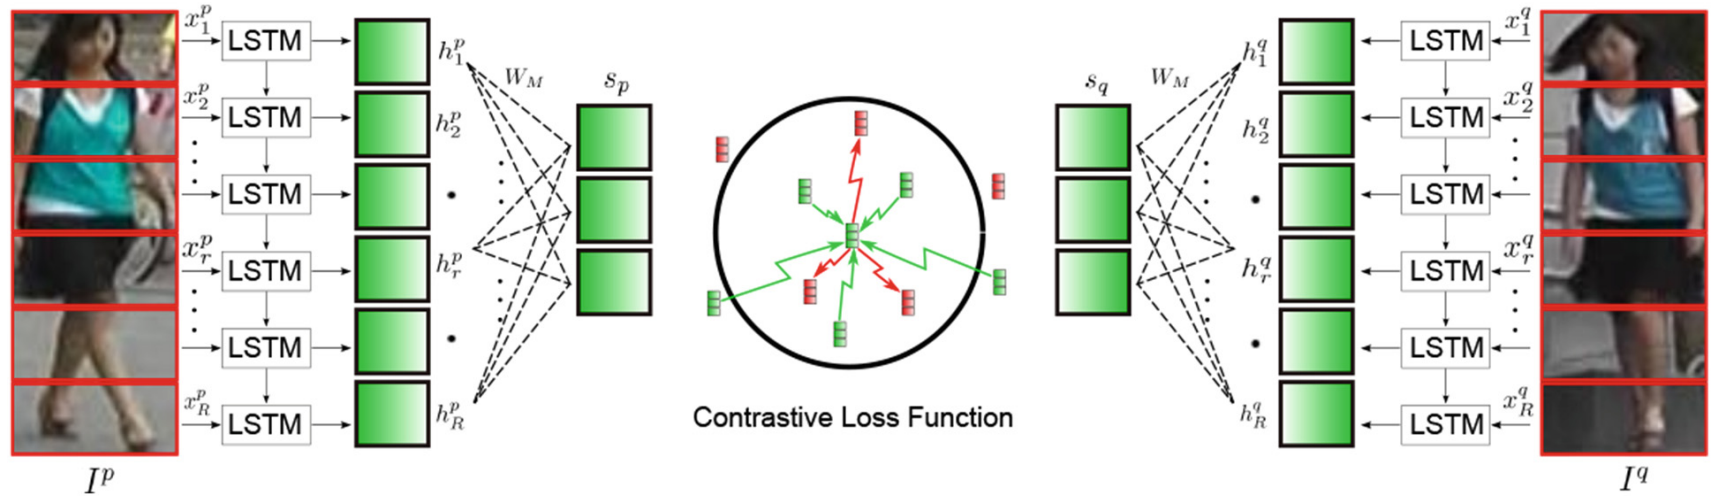
\includegraphics[width=1\linewidth]{切片.png}
  \caption{图片垂直切割后输入LSTM(Long Short-Term Memory)网络后进行特征提取}
  \label{fig:part}
\end{figure}

基于视频序列的Re-ID方法最主要特点是这类方法不仅考虑了图像的内容信息,还考虑了帧与帧之间的运动信息、时序信息等。这类方法主要基于利用CNN提取空间特征的同时,也要利用循环神经网络提取时序特征。 累计运动背景网络(Accumulative Motion Context Network, AMOC)\cite{liu2017video}是代表方法之一,其核心思想在于网络除了要提取序列图像的特征,还要提取运动光流的运动特征,最后再输入RNN来提取时序特征。于是,通过AMOC网络,每个图像序列都能被提取出一个融合了内容信息、运动信息的特征。



\subsection{多摄像头行人位置估计算法}

与单目行人检测算法相比,多摄像头行人位置估计通常来看具有更好的效果,因为多个视角很适合解决复杂遮挡问题\cite{baque2017deep}。

概率占据图方法(Probabilistic Occupancy Map method, POM)\cite{fleuret2007multicamera}通过从多个视角中发掘其中的几何约束,从而得到行人在地面的位置概率的生成模型。POM是在平均场推断常常被自然地用于处理遮挡问题的背景下产生的。同时,为了利用视频的时序信息,概率占据图方法常常与凸最大成本流优化(Convex Max-cost Flow Optimization)\cite{berclaz2009multiple}相结合,应用于行人跟踪的问题中。

在行人比较拥挤的场景中,Ge\cite{ge2010crowd}等人提出采用随机人群配置的随机生成过程建模,然后使用最大后验概率估计来寻找图像观测值的最佳拟合。而Chavdarova\cite{chavdarova2017deep}等人则提出了DeepMCD(Deep Multi-camera Detection)算法,这种方法集成了CNN得到的特征图,并展示了CNN分类器的准确性和可信度可以随着摄像头视角的的增加而提高。为了缓解数据需求问题并提高泛化能力,作者首先使用较大的单目数据集——Caltech数据集\cite{dollar2009pedestrian}来训练得到基础处理网络。之后,CNN被用来使用从基础处理网络中得到的权重数据,并通过并行(Multi-view Stream)的方法处理得到最终的估计结果。作为这种方法的优化,Chavdarova等人后续又在\cite{chavdarova2017deep}中提出了两种多视角数据负挖掘的架构,来更好地训练这种网络。

目前,有一些多视角技术考虑对目标场景进行额外的训练步骤,以更好地利用应用场景中上下文信息。但由于对每个特定场景训练有着很大的隐藏成本,所以我们可以将其归类为不可泛化的方法\cite{lima2021generalizable}。在这个意义上,Baque等人\cite{baque2017deep}提出将卷积神经网络(CNN)和条件随机场(Conditional Random Field, CRF)相结合的方法,以处理观察到的行人之间难以匹配的问题,即深度遮挡推理方法\cite{baque2017deep}。这种方法利用CNN和CRF相结合的体系结构和平均场推理,用类似\cite{fleuret2007multicamera}中的方式来生成概率占用图(POM),同时,还利用了CNN提取出来的判别特征。它引入了高阶CRF的方法,其中一元项由CNN的ROI pooling过程产生\cite{faster2015towards},高阶项则是由解释遮挡的生成网络的预测和能判断身体部位图像块的CNN的预测的差异来计算。这个方法需要在特定的WildTrack数据集上训练的东西太多,其对每个地面计算检测框的精读会受到网格大小的限制;此外,WildTrack数据集直接提供了地面分割的标注,但是一般的数据集只给位置不给地面分割的标注,导致这个方法的在数据集上的应用有一定的局限性;同时,它检测框的估计需要先验知识,例如人的高度等。此外,MVDet\cite{hou2020multiview}通过特征的透视变换将不同视角的行人热图放置在同一个坐标空间中,从而整合了多个视角的检测信息。类似的,DMCT\cite{you2020real}提出了透视感知网络(Perspective-aware Network),从而生成了与摄像机视角相关的探测区信息,之后,通过数据融合得到地面的占据热图(Occupancy Heatmap)估计,最后再利用Deep Glimpse Network得到行人的位置。

\section{论文结构安排}

本文的主要工作是完整搭建了一个多摄像头行人位置估计系统。这个系统包含单目行人检测、相机投影、对位置建立高斯概率分布模型、聚类进行数据融合、特征提取和训练等部分。最终在WildTrack数据集上达到了令人满意的行人位置估计结果。

第一步,行人检测系统。其功能是对输入的多个摄像头的WildTrack数据集图片进行推断,以得到每张图中每个人行人的姿态节点,是后续计算行人位置的基础步骤。这一步选择了目前单目摄像头综合预测结果最好的AlphaPose\cite{fang2017rmpe, li2018crowdpose, xiu2018poseflow}模型。之后,提取WildTrack数据集中的各个摄像头视频帧,并进行去畸变和推断真值的预处理,作为训练集的扩充。最后利用AlphaPose对上述图片进行推断,得到行人姿态节点。

第二步,利用相机投影对位置建立高斯概率分布模型。在这一步中,先利用每个视角得到的人物姿态节点计算出每个视角每个人行人在当前图片中的2D足点(即双脚之间所站立的位置点),再利用每个摄像头的相机参数以及相机投影关系,得到3D平面上每个行人的3D足点。最后,以每个3D足点为中心,结合摄像头视角方向,建立二维高斯概率分布作为对每个行人位置的估计。

第三步,利用层次聚类方法进行数据融合,并调整参数。将高斯概率之间的KL散度(KL Divergence)作为各个点之间的距离,利用层次聚类的方法,将每个行人在不同摄像头下得到的二维高斯概率分布进行融合,最终得到所有行人位置的粗略估计。通过对估计结果的优化,反过来调整前述二维高斯概率分布和层次聚类的超参数,从而优化后续步骤的输入。

第四步,生成热图和标签,然后进行训练和实验结果评测。首先,将第三步中得到的二维高斯概率分布处理为可供神经网络输入的热图,然后利用WildTrack数据集的实际标注得到与热图同样大小的黑白标签图。最后,输入分割模型ResUnet++\cite{jha2019resunet}进行特征提取和训练,最终在WildTrack官方图片上测试,得到实验结果。

接下来对本文各个章节结构安排进行说明。

\begin{enumerate}
  \item 第一章,引言。首先对本文所关注的问题进行描述,并对问题进行初步分解。然后阐述本课题研究的实际意义和价值,指出本文在这个问题中所关注的技术难点和突破口。最后对本课题当前的研究背景和现状加以说明,并对涉及到的相关技术和领域进行简要概括和梳理,主要包括单目行人检测算法、行人重识别算法和多摄像头行人位置估计算法。
  \item 第二章,行人检测与高斯概率分布建模。本章中主要介绍主要工作中行人检测系统的应用、数据的预处理、数据集的扩充和利用相机投影对位置建立高斯概率分布模型的过程。首先将会介绍本文工作所采用的行人检测算法,以及该方法的优势,之后会介绍如何对WildTrack数据集进行扩充和预处理,包括真值推断和消除畸变等。最后,阐明利用相机参数进行相机投影和对位置建立高斯概率分布的原理和细节。
  \item 第三章,数据准备与深度学习方法构建。本章中,首先介绍如何对各摄像头数据进行融合,并构建层次聚类方法得到粗略的行人位置估计,然后介绍如何通过粗略的估计结果反向优化高斯概率分布和层次聚类的超参数。同时,将会介绍利用扩充和预处理后得到的WildTrack数据集制作适合网络输入的热图和标签图。最后,将会对所采用的深度学习方法和神经网络进行说明。
  \item 第四章,评价指标与实验结果。本章主要对结果的几个评价指标进行介绍,同时介绍实验结果,并对实验结果做出分析。
  \item 第五章,结论。从本文所关注的问题和研究目的出发,对研究过程和结果进行总结,思考整个实验的不足之处,并提出未来可能的改进方向。
\end{enumerate}

% !TeX root = ../thuthesis-example.tex

\chapter{行人检测与高斯概率分布建模}

\section{数据集扩充和预处理}

对于行人检测与高斯概率分布建模,首先需要选择合适的数据集,并对数据进行预处理。目前,比较适合多摄像头多目标位置估计的综合性能较好的数据集主要包括Duke MTMC(Multi-Target, Multi-Camera)数据集\cite{Ristani2016PerformanceMA}和上文提到的WildTrack数据集。其中,Duke MTMC数据集是2014年杜克大学校园拍摄的监控视频片段的数据集,用于视频跟踪系统、行人重识别和低分辨率面部识别的研发。这个数据集包含超过14小时的来自8个摄像头的同步监控视频,视频为1080p和60fps,超过200万帧,其中共有2000名学生步行上下学。但由于英国《金融时报》调查发现此数据集可能侵犯个人隐私,Duke MTMC数据集关闭了下载渠道。而WildTrack数据集则是一个记录了苏黎世联邦理工大学主楼外的学生的监控录像数据集。WildTrack使用七个具有重叠视野的高科技静态定位摄像头(三个GoPro Hero 4和四个GoPro Hero 3摄像头)获取,具有高精度的联合摄像机校准以及视图序列同步,并且摄像头视野有着较大部分的重叠。因此可以满足在多视角多目标位置估计问题中大规模多摄像头数据集深度学习训练的需要。

本文采用WildTrack数据集。此数据集提供了时长为35分钟的分辨率为$1920\times1080$、帧率为60fps的来自七个摄像头的同步视频,以及分辨率为$1920\times1080$、帧率为2fps并消除畸变后的400张视频帧(如图~\ref{WildTrack_Cam}所示),并且提供了400张视频帧的行人位置标注,最后,还提供了每个摄像头的相机参数。此数据集所关注的区域为$1200cm\times3600cm$广场,而在标注时,将广场分割为$480\times1440$的网格,每个网格边长为2.5cm,从而得到691200个网格点。对每个网格点从上到下从左到右进行编号,可以得到网格编号,称为Position ID。若在此网格上建立直角坐标系,坐标以米为单位,原点在$(-3.0, -9.0)$处,从而,根据Position ID可以得到标注坐标为
\begin{equation*}
  \left\{
    \begin{aligned}
    X = & -3.0 + 0.025 \times \text{Position ID} \% 480 \\\
    Y = & -9.0 + 0.025 \times \text{Position ID} / 480
    \end{aligned}
  \right.
\end{equation*}


\begin{figure}
    \centering
    \subcaptionbox{\label{cam1}}
      {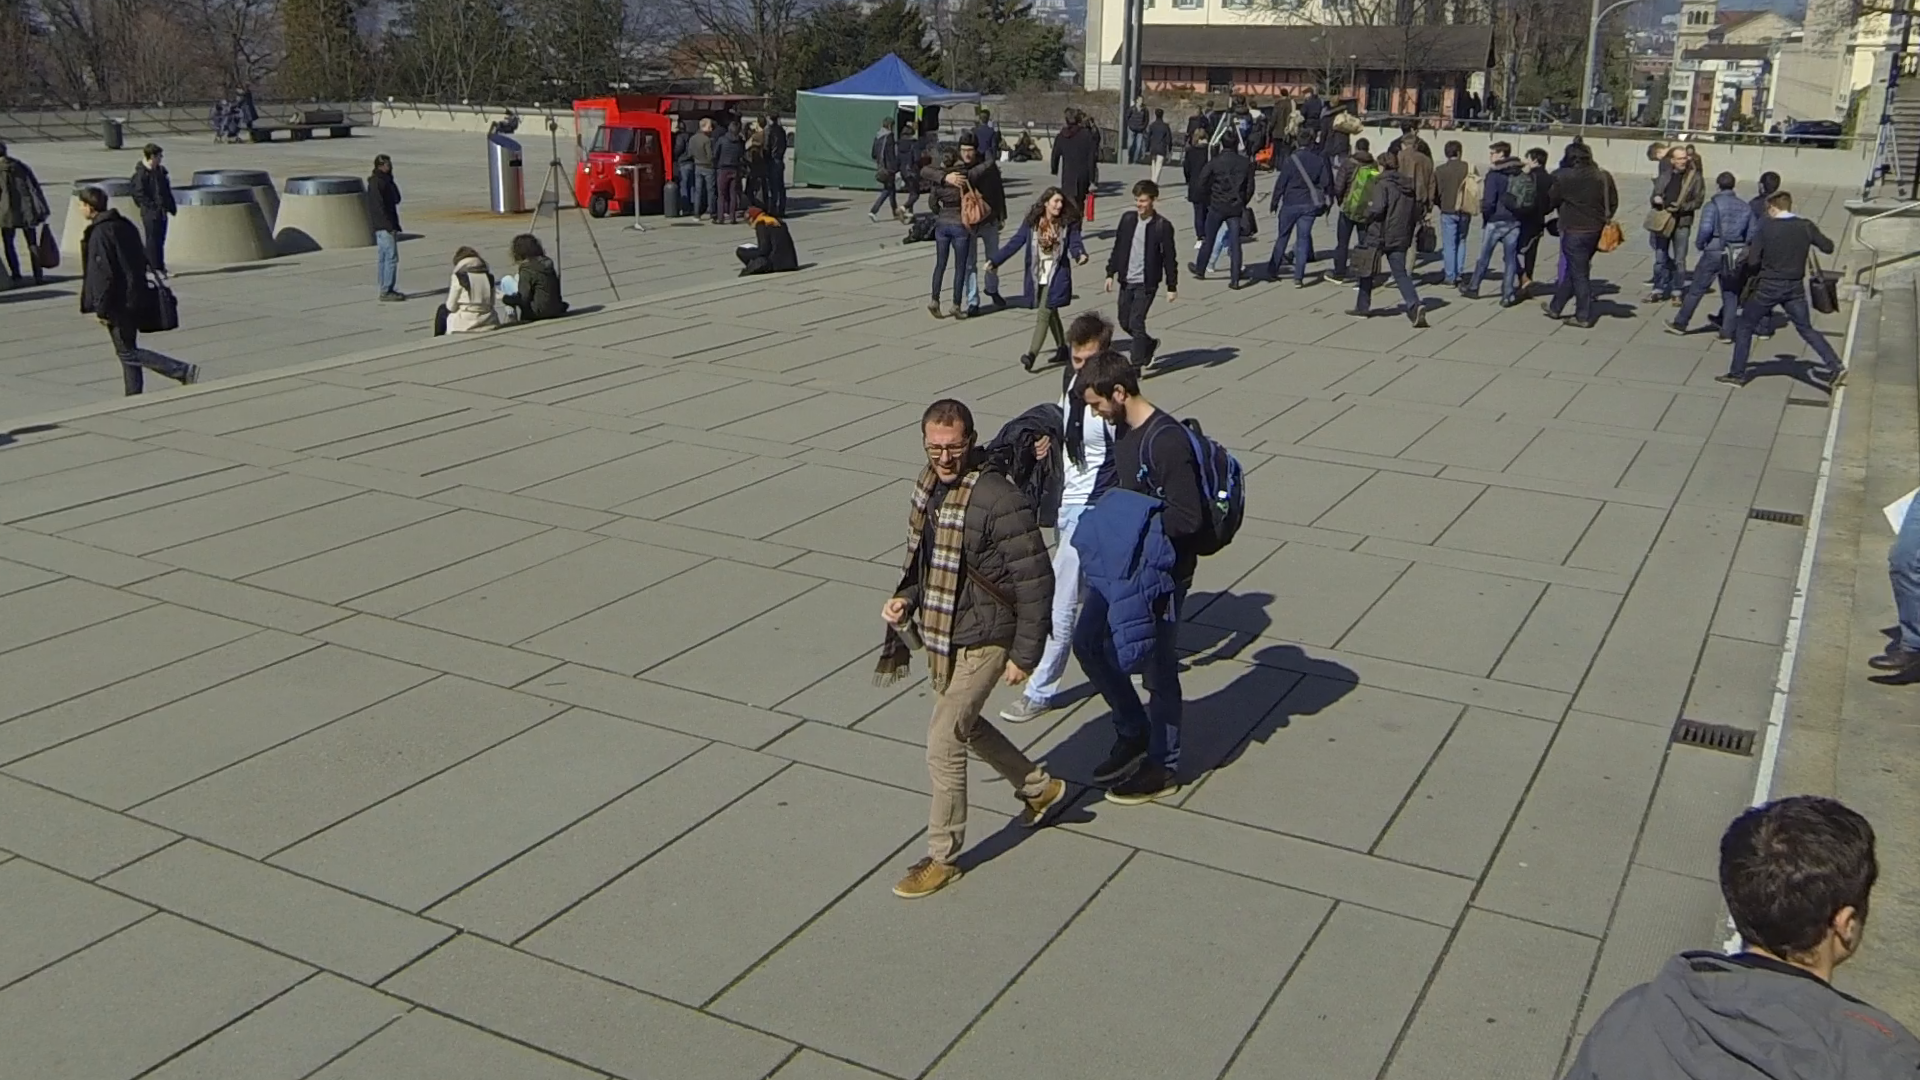
\includegraphics[width=0.3\linewidth]{cam1.png}}
    \subcaptionbox{\label{cam2}}
      {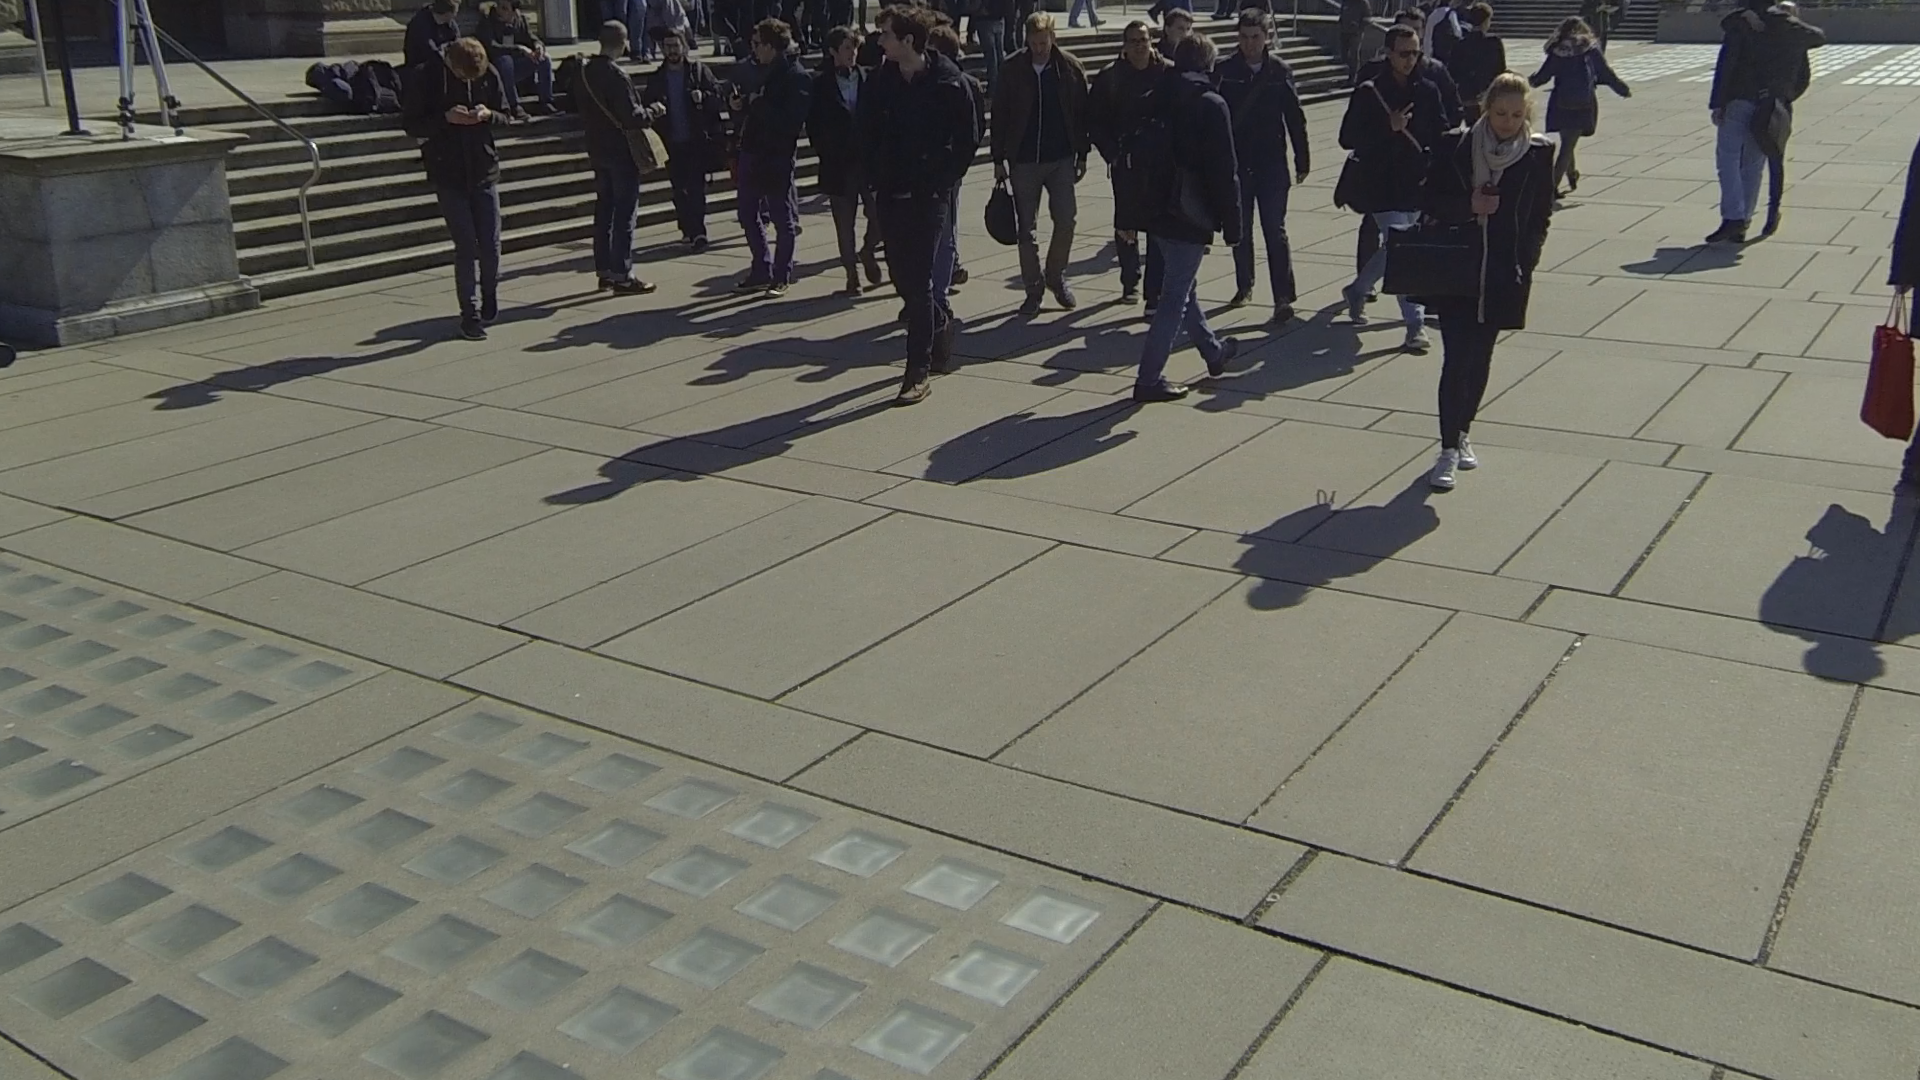
\includegraphics[width=0.3\linewidth]{cam2.png}}
    \subcaptionbox{\label{cam3}}
      {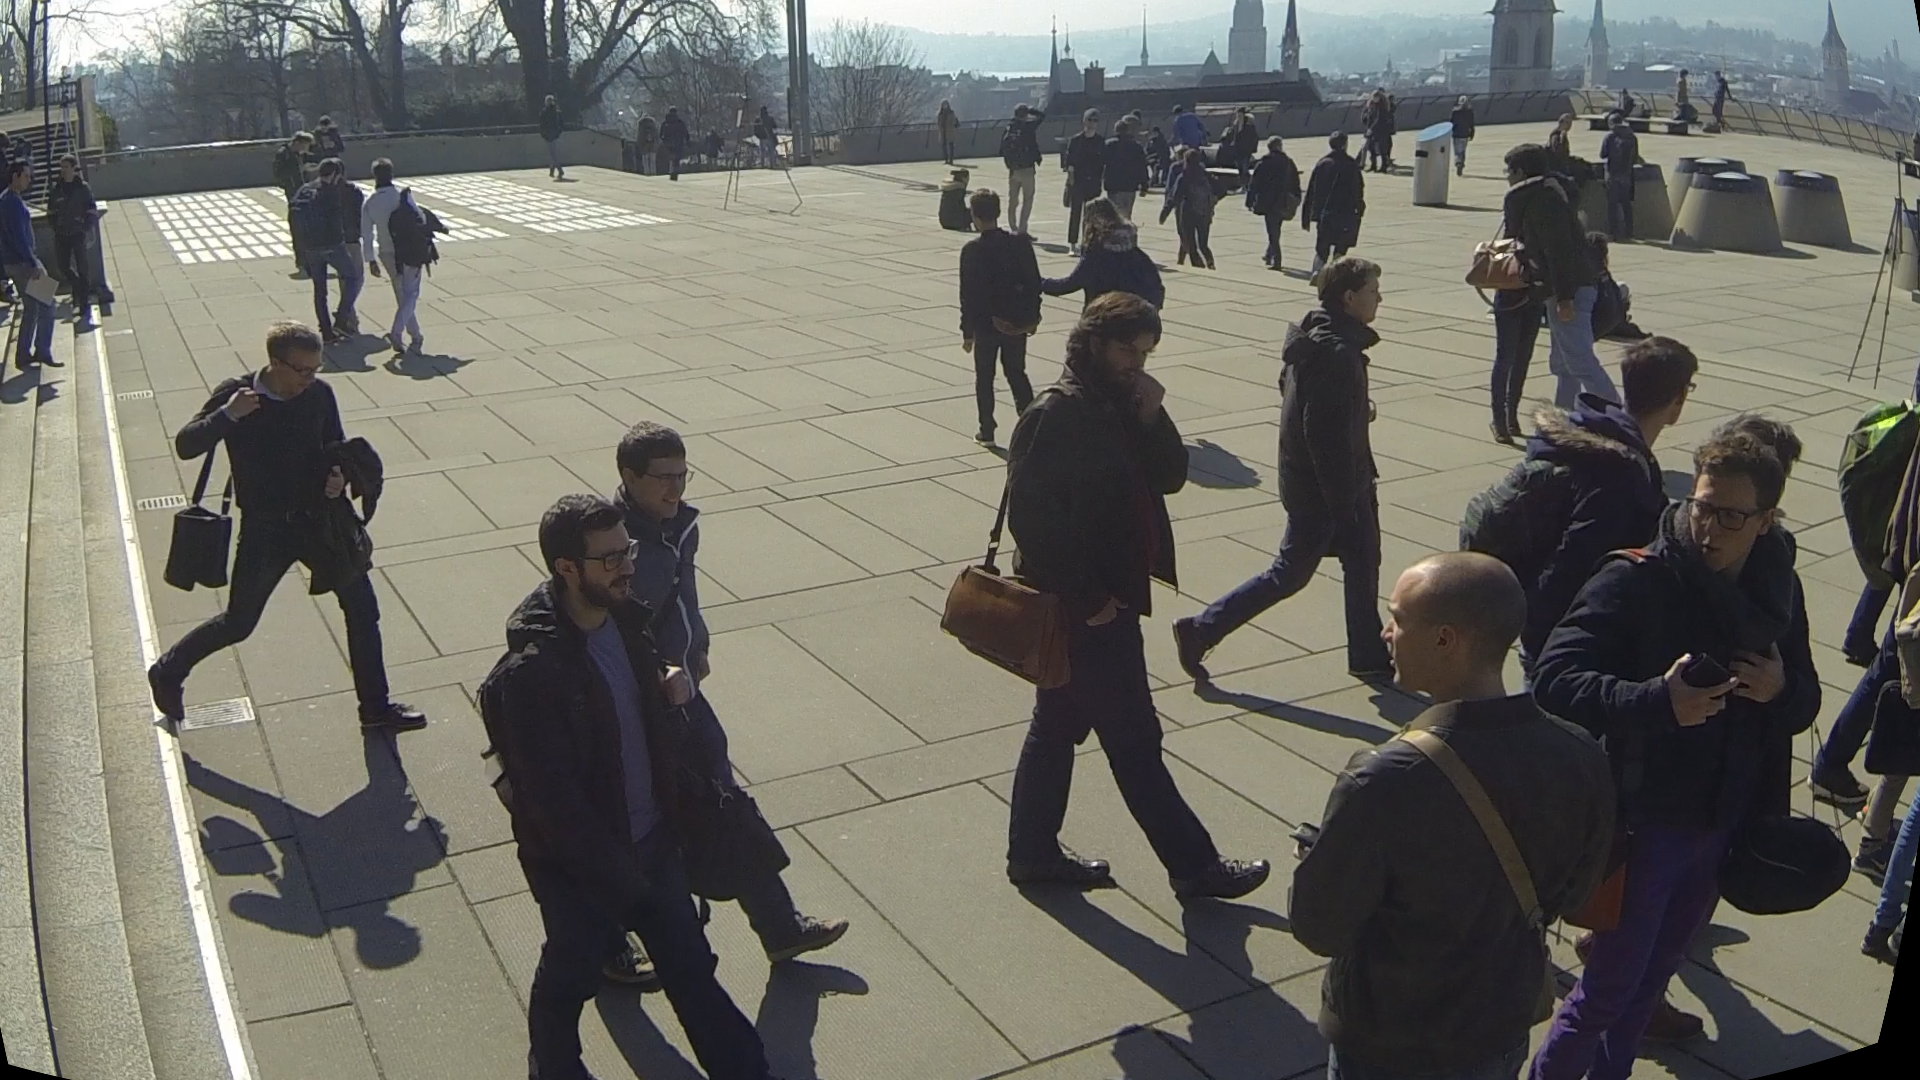
\includegraphics[width=0.3\linewidth]{cam3.png}}
    \quad
    \subcaptionbox{\label{cam4}}
      {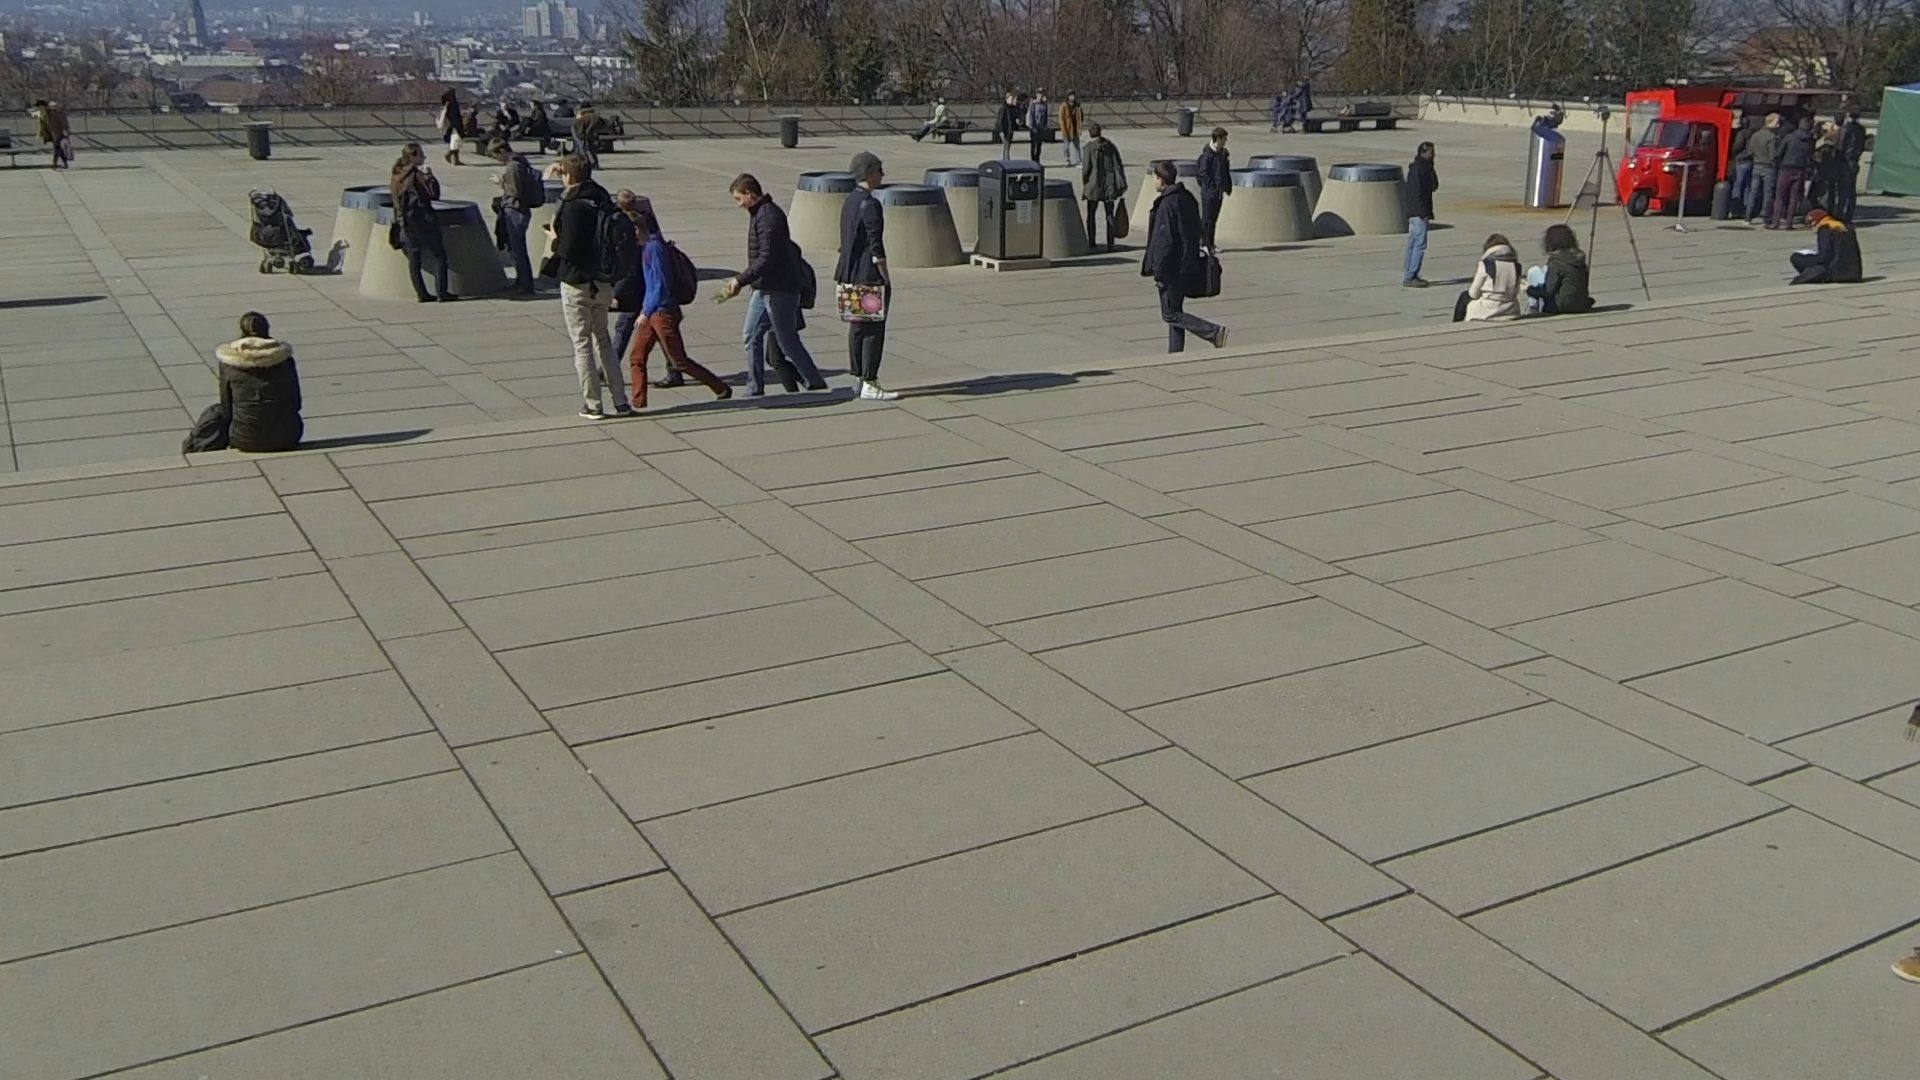
\includegraphics[width=0.3\linewidth]{cam4.png}}
    \subcaptionbox{\label{cam5}}
      {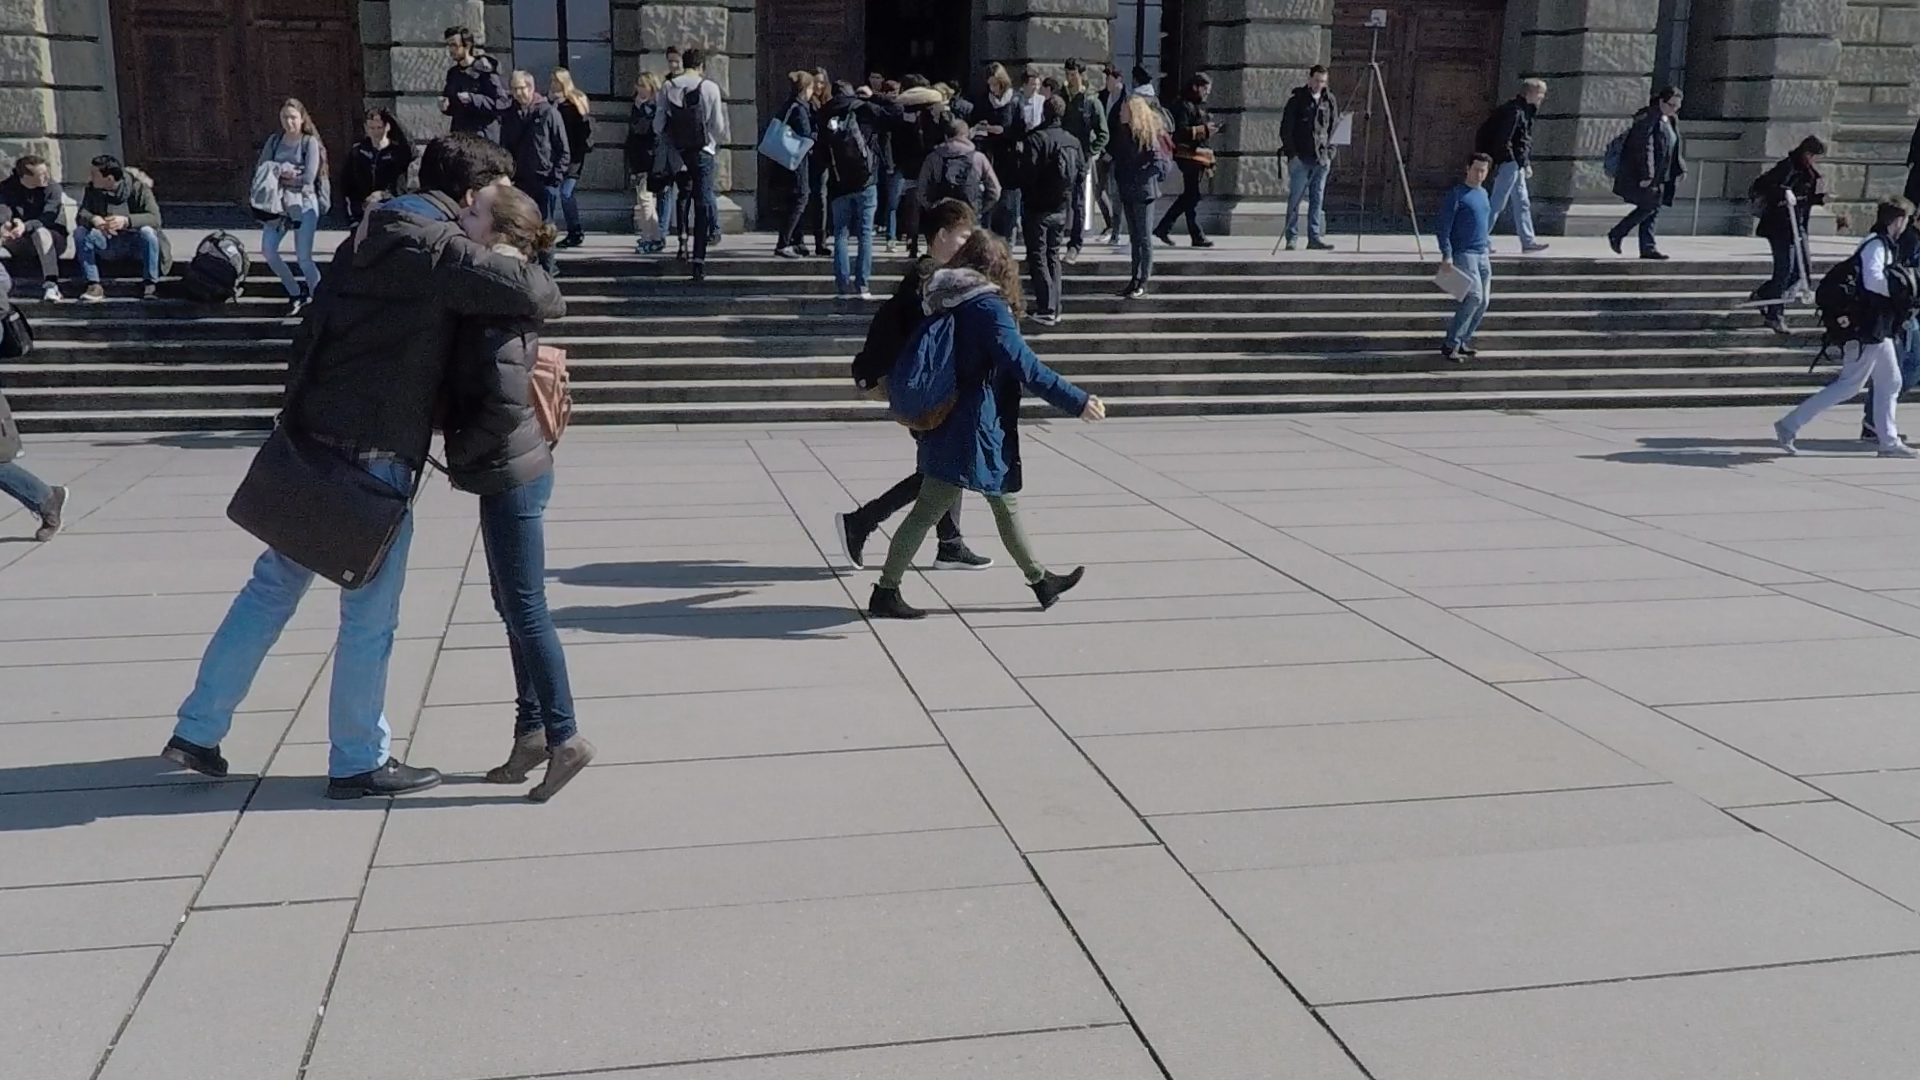
\includegraphics[width=0.3\linewidth]{cam5.png}}
    \subcaptionbox{\label{cam6}}
      {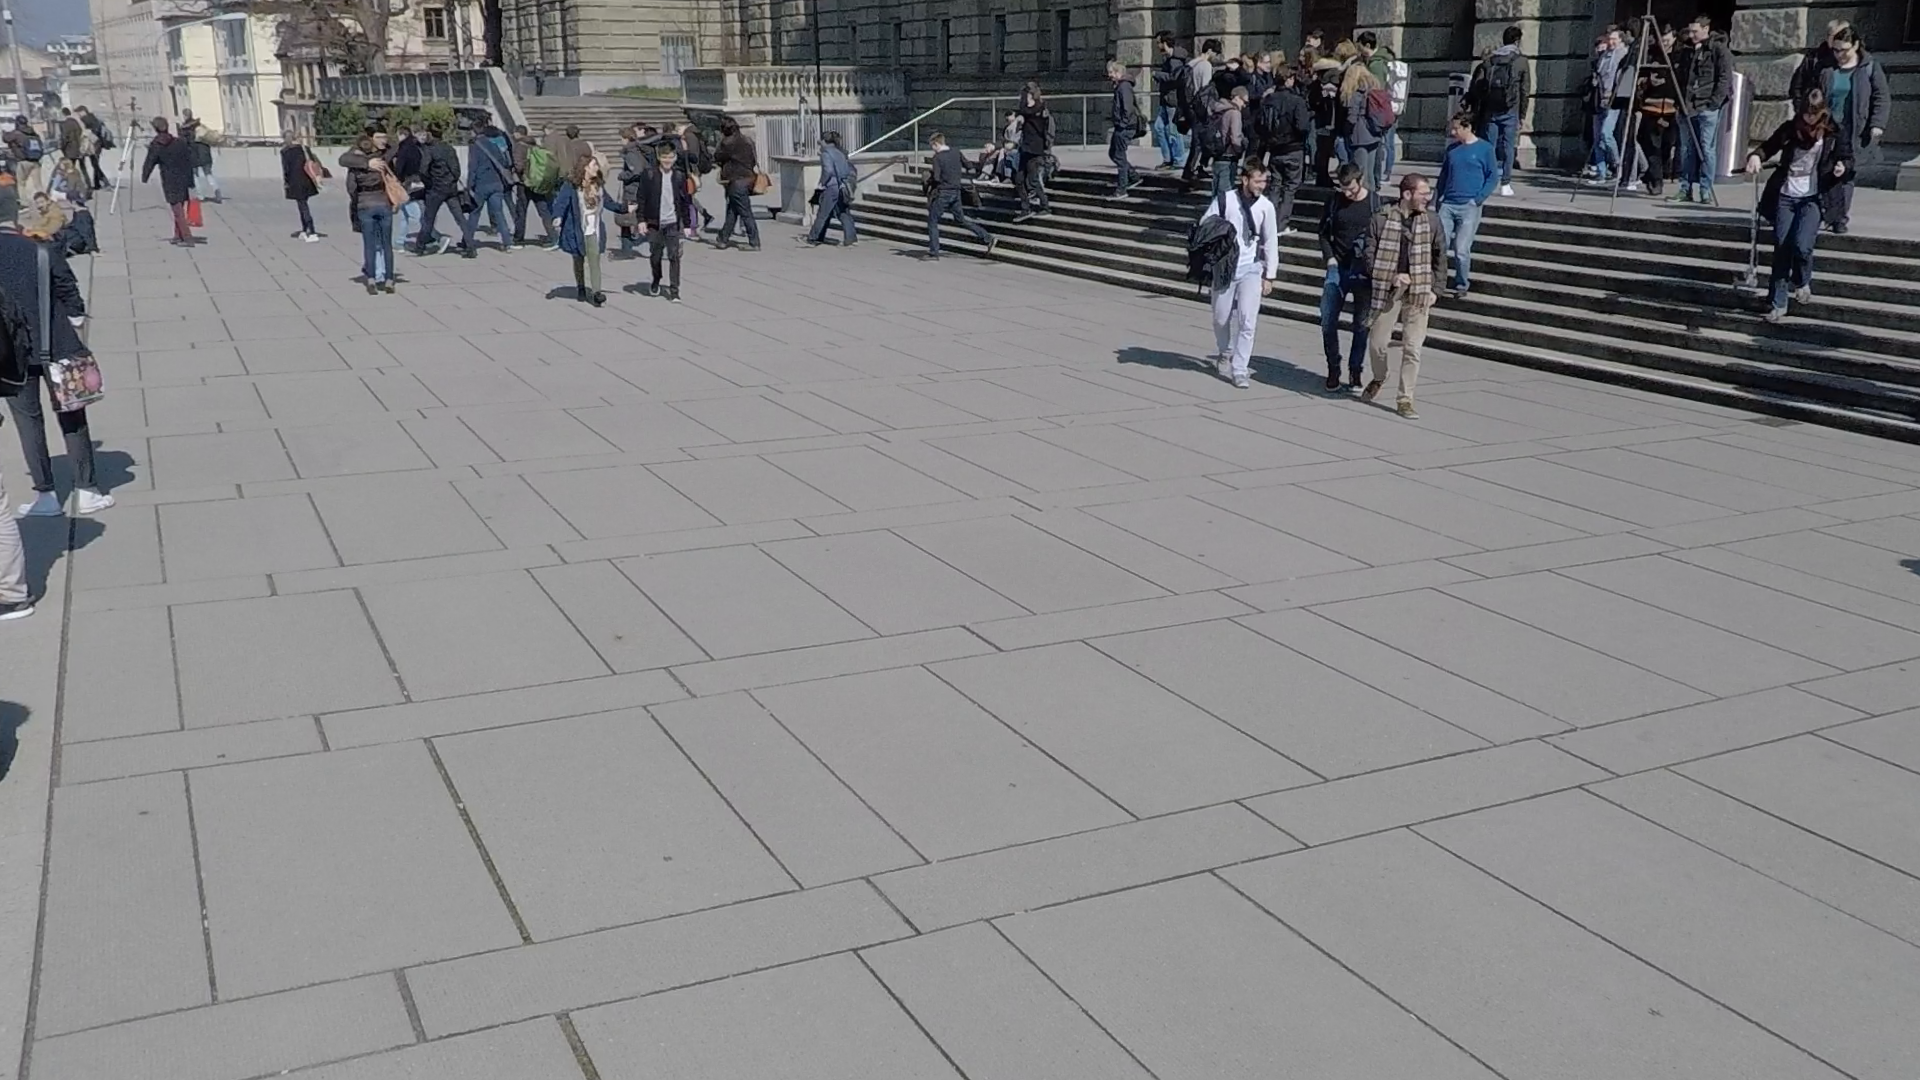
\includegraphics[width=0.3\linewidth]{cam6.png}}
    \subcaptionbox{\label{cam7}}
      {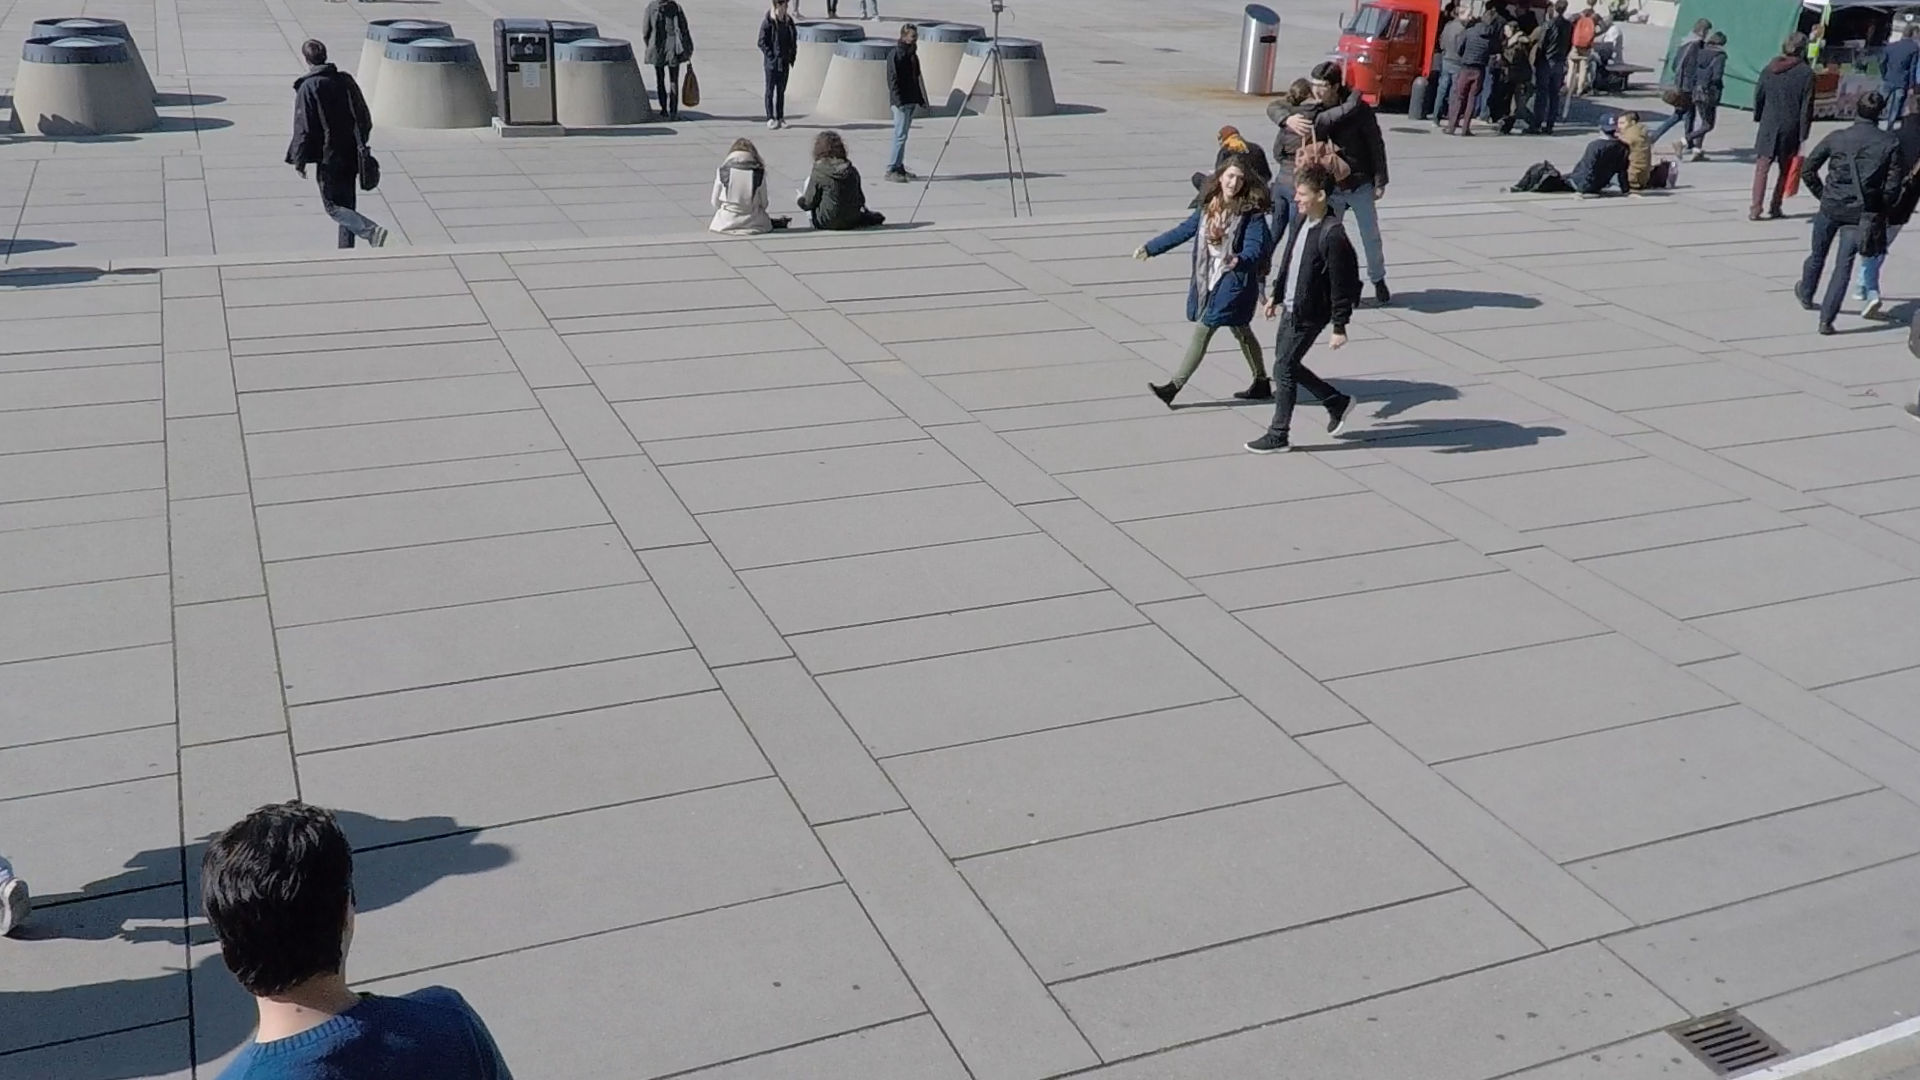
\includegraphics[width=0.3\linewidth]{cam7.png}}
    \caption{WildTrack数据集中来自七个摄像头的图片}
    \label{WildTrack_Cam}
\end{figure}

由于后续神经网络训练的需要,而官方提供的400张图片和标注总体数量太少,难以达到预期训练效果,因此需要使用WildTrack数据集提供的视频进行数据集的扩充。由于带标注的400张图片帧率为2fps,而视频序列的帧率则为60fps,因此,可以先从视频序列中找到与官方提供的图片集一致的帧,以此帧为起点,每30帧就会再次遇到官方图片集中的下一张图片。但是,由于从视频序列中提取的帧在WildTrack数据集中并不提供真值标注,因此可以通过对提供标注的400张图片集的标注进行插值,从而推断得到每两个图片之间提取到的视频帧的真值标注。此外,由于提供的图片集已经被去畸变处理过,而提取到的视频帧并未去畸变处理。故需要先对视频帧进行与图片集相同的去畸变处理,如图~\ref{undistortion}所示。

\begin{figure}
  \centering
  \subcaptionbox{\label{before}}
    {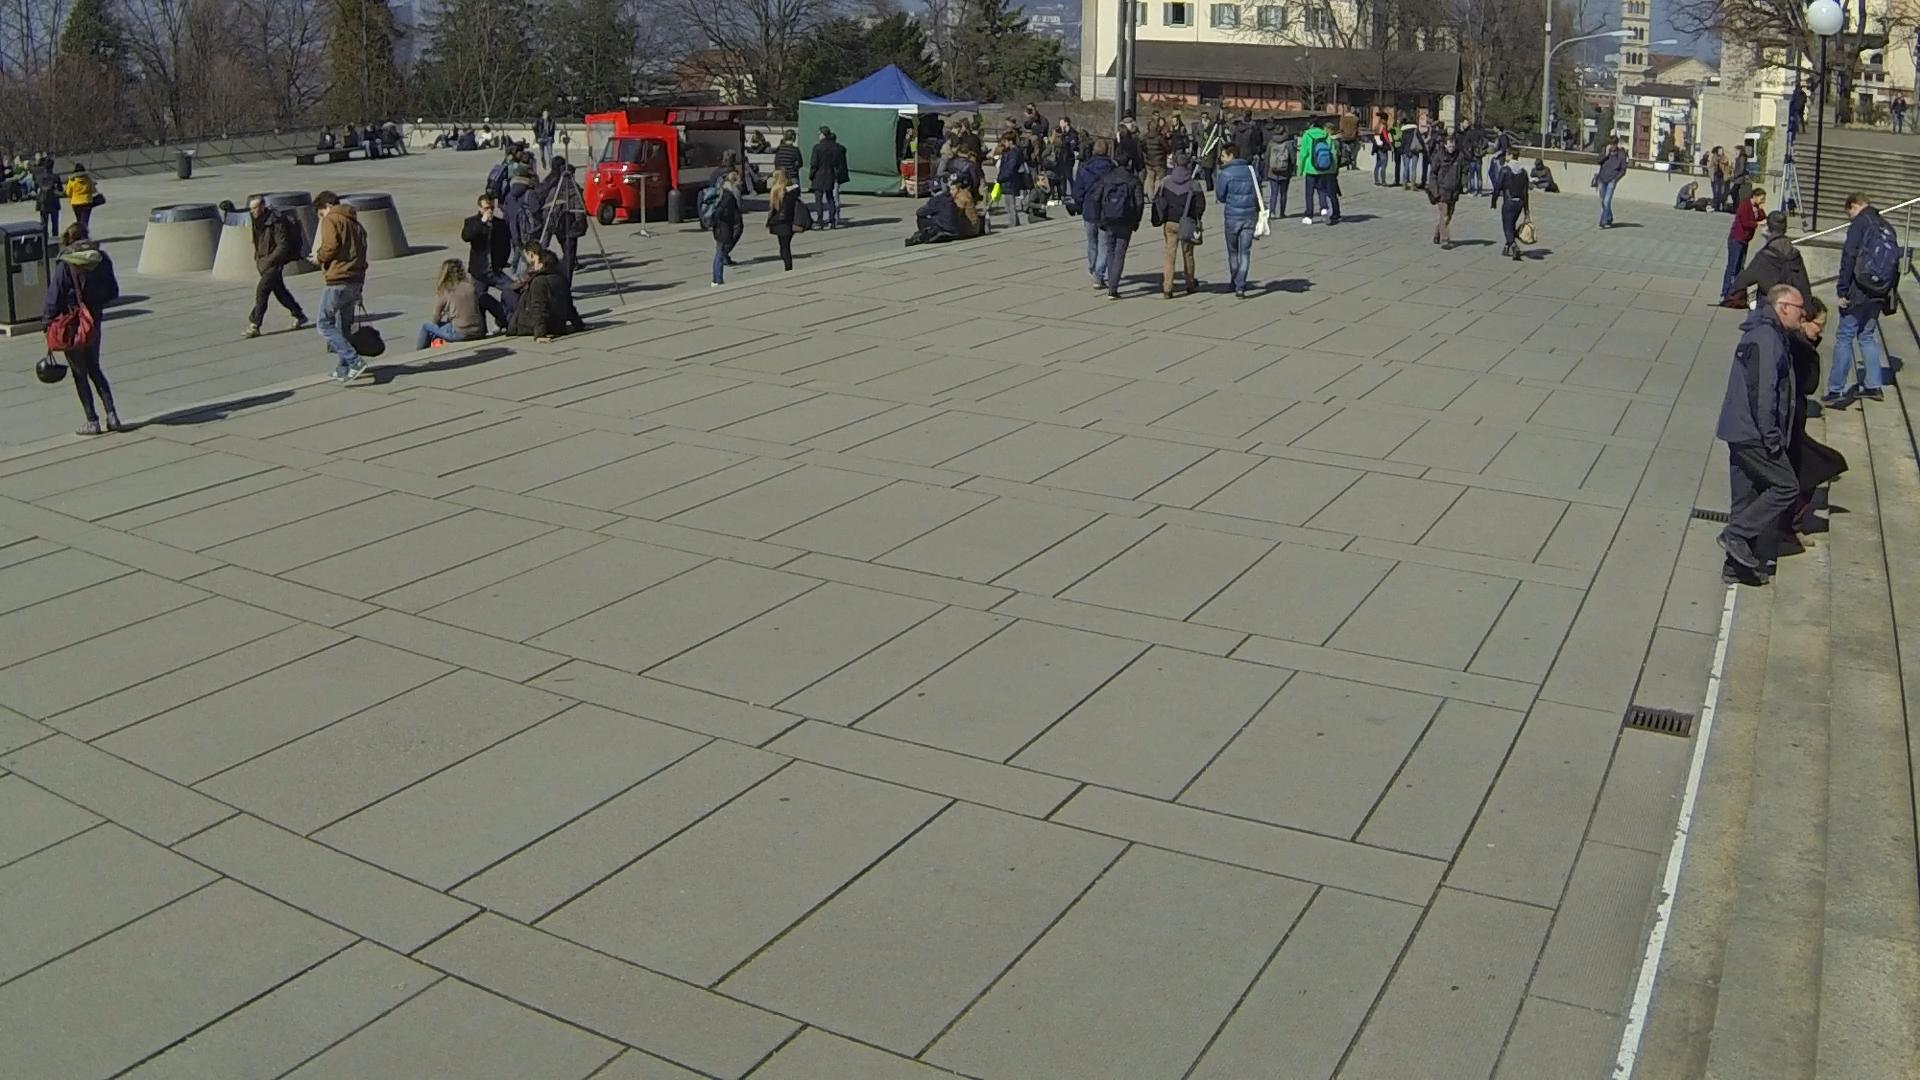
\includegraphics[width=0.4\linewidth]{before_undistort.jpg}}
  \subcaptionbox{\label{after}}
    {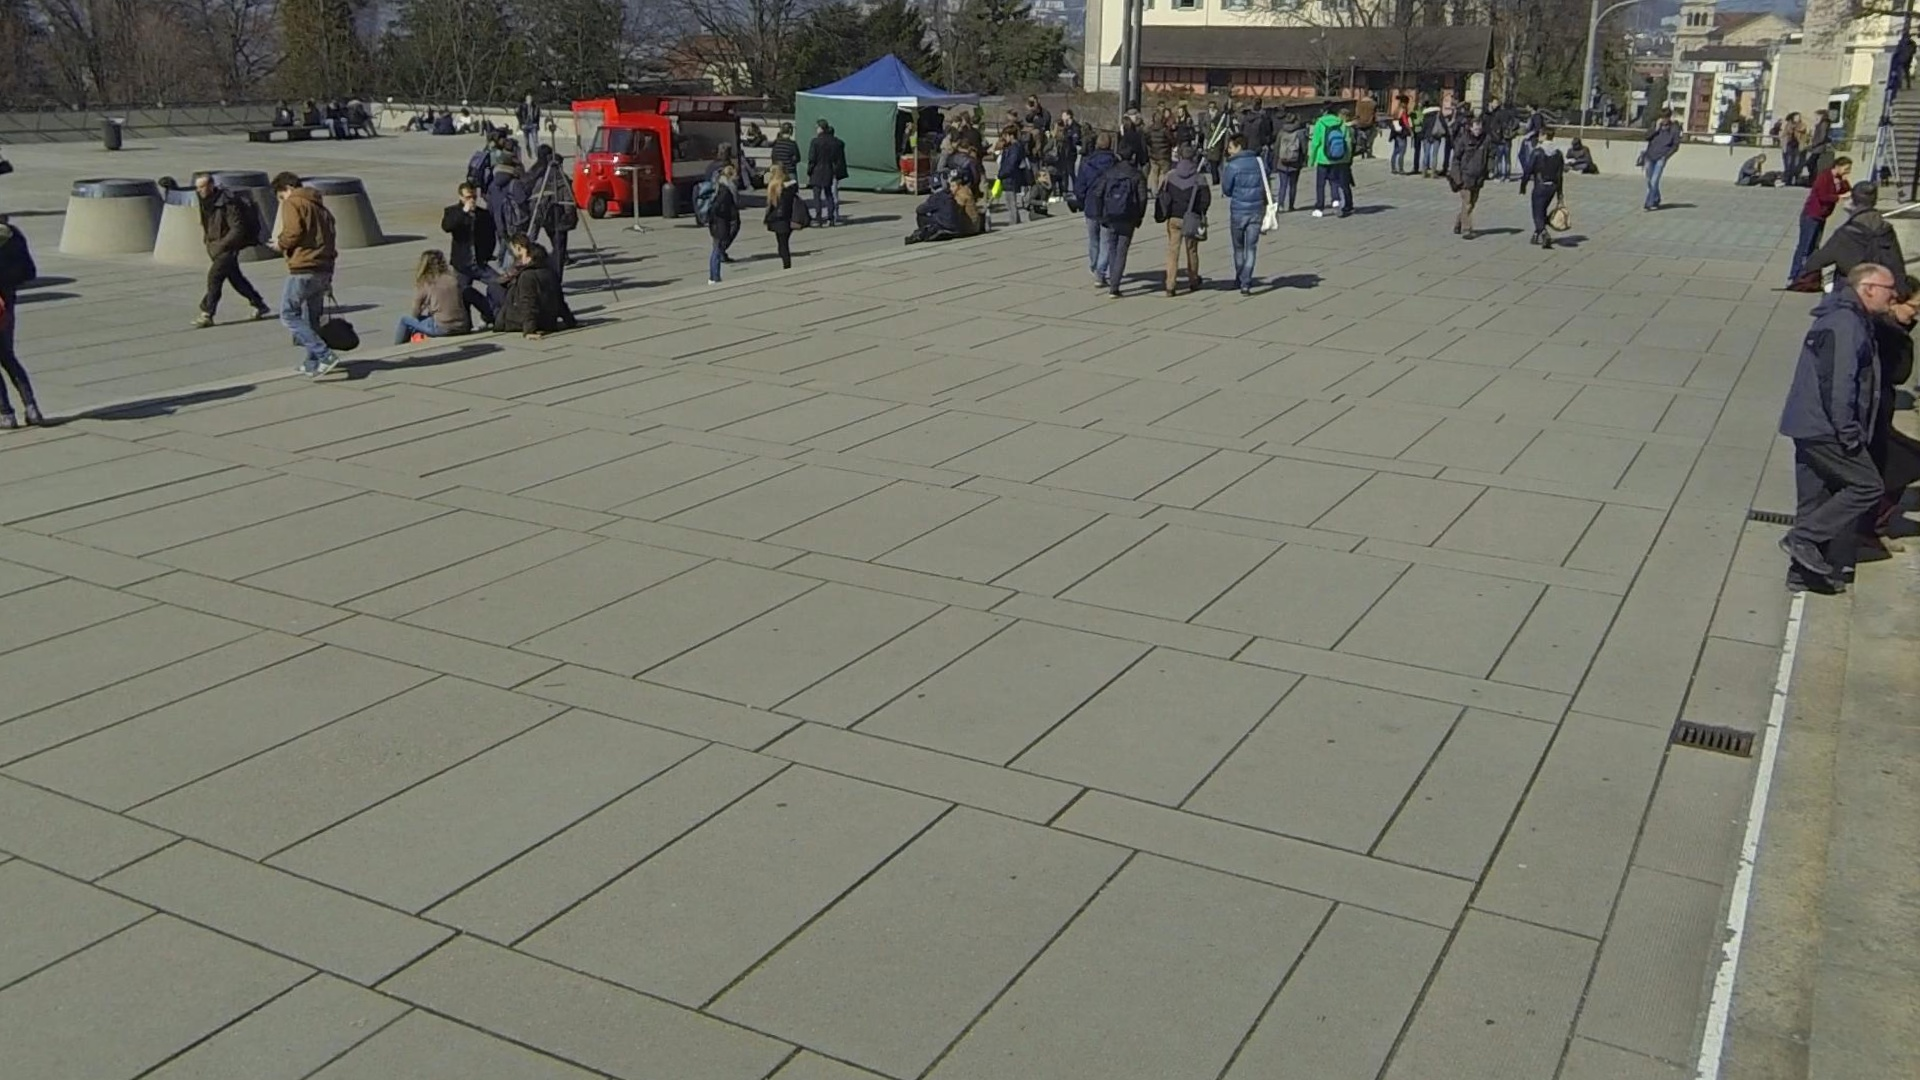
\includegraphics[width=0.4\linewidth]{after_undistort.jpg}}
  \caption{去畸变处理示例}
  \label{undistortion}
\end{figure}

针孔摄像机会引起图像的严重畸变,主要有径向畸变和切向畸变。径向畸变使直线看起来是曲线。离图像中心越远,图像的径向畸变越大。径向畸变可以表示为:
$$
\begin{aligned}
x_{\text{distorted}} = & x(1+k_{1}r^{2}+k_{2}r^{4}+k_{3}r^{6}) \\\
y_{\text{distorted}} = & y(1+k_{1}r^{2}+k_{2}r^{4}+k_{3}r^{6})
\end{aligned}
$$
同样,切向畸变是由于摄像镜片与成像平面不完全平行造成的。因此,图像中的某些区域可能看起来比预期的更近。切向畸变量可表示为:
$$
\begin{aligned}
x_{\text{distorted}} = & x+[2p_{1}xy+p_{2}(r^{2}+2x^{2})] \\\
y_{\text{distorted}} = & y+[p_{1}(r^{2}+2y^{2})+2p_{2}xy]
\end{aligned}
$$
故需要得到五个畸变参数:
$$
\text{distortion coefficients} = (k_{1}, k_{2}, p_{1}, p_{2}, k_{3})
$$
这些畸变参数一般需要标定求得。但在本文中,由于WildTrack数据集提供了每个相机的畸变参数,因此我们可以直接使用,无需标定。
除此之外,还需要相机内外参数。其中,内部参数是特定于照相机的,包括像焦距$(f_{x},f_{y})$和光学中心$(c_{x},c_{y})$等信息,从而可以创建相机的内参数矩阵(Camera Intrinsics)K,以消除由于特定相机的镜头畸变。相机矩阵是特定于相机的,因此得到后可以在同一相机拍摄的其他图像上重复使用。相机矩阵可表示如下:
$$
K=
\left[
\begin{matrix}
f_{x} & 0 & c_{x} \\\
0 & f_{y} & c_{y} \\\
0 & 0  & 1
\end{matrix}
\right]
$$
而外部参数对应于旋转和平移矢量。实际上,WildTrack数据集也已经提供了每个摄像机的相机内外参数。利用这些参数,我们可以通过经典的去畸变算法,实现对视频提取帧的去畸变操作。由于相机参数未变,所以去畸变处理后视频帧中背景状况与官方提供的图片集背景状况完全一致。至此,完成了数据的扩充和预处理操作。

\section{行人检测算法}

本文中的行人检测算法主要依赖于现成的不需要针对特定场景进行训练的单目行人检测器。从单目检测器得到的行人姿态节点中,我们可以计算出每个行人的足点(即双脚之间所站立的位置点)。后续便可以使用此足点进行数据融合,从而得到三维平面上的位置估计结果。

单目检测器实际上有很多算法,如引言中提到的基于运动检测的经典算法如高斯混合模型分离算法、VIBE算法和CodeBook算法等,但这些传统算法很容易受到环境和背景噪声的影响,而且不能检测静止目标,在机器学习方法迅速发展的今天已逐渐过时。因此,本文主要在机器学习算法尤其是深度学习方法中进行选取。在主要使用深度学习方法的算法中,一些单目检测器可以同时提供人物的检测框和姿态节点\cite{li2019crowdpose}。这些方法对全身姿态节点的使用可以更有效地处理遮挡问题,因此,我们选用了目前综合性能最好的AlphaPose。在AlphaPose提供的多种模型中,本文选取了以ResNet152为骨干(Backbone),以YOLOv3为探测器,基于MSCOCO数据集\cite{lin2014microsoft}进行训练得到的Fast Pose(DUC)\cite{fang2017rmpe, li2018crowdpose, xiu2018poseflow}模型。这个模型将输入摄像头拍摄的尺寸为 $256 \times 192$ 的图片,输出每张图片中每个人的姿态节点。其中,人物姿态节点的表示方式与MSCOCO数据集\cite{lin2014microsoft}中姿态表示相同,即包含17个姿态节点。在这些节点中,本文只使用了两个脚踝的节点,具体而言,保留了高于阈值 $t_s$ 的脚踝节点。但由于脚踝节点高于地面,并不能代表人的位置,故可以利用两个脚踝节点计算得到一个抵消项$\delta$,如下所示:
\begin{equation*}
 \delta = bb_{y_{max}} - max(la_y, ra_y)
\end{equation*}
其中,$bb_{y_{max}}$为当前行人的检测框下沿的纵坐标,而$la_y$和$ra_y$则分别是行人的左脚踝节点和右脚踝节点。因此,如图~\ref{GroundPoint_Compute}所示,其中红色点为行人姿态节点,蓝色点为行人脚踝节点(Ankle),黄色点为脚踝中点(Midpoint),绿色点为足点(GroundPoint),可见,通过中点向下偏移$\delta$便可以计算得到行人的足点。
\begin{figure}
    \centering
    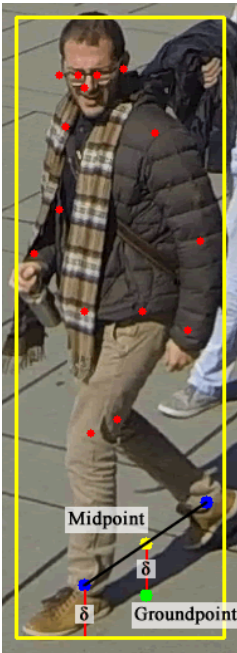
\includegraphics[width=0.2\linewidth]{GroundPoint_Compute.png}
    \caption{行人足点计算实例}
    \label{GroundPoint_Compute}
\end{figure}
根据上述方法,便可输入所有需要的图片或视频数据,推断出每帧中每个行人在此帧上的足点位置坐标,作为后续三维位置推断的基础。

\section{相机投影原理}

在行人检测中,得到每帧每个行人在当前帧的足点位置坐标后,接下来需要推断得到行人在实际地面上的坐标。这里主要使用几何约束和相机投影关系来实现。

相机成像的过程可表示为
$$ \bm{p} = K\bm{P}_{c} $$
其中,$\bm{p}=(\mu, \nu)$是图像中像点的像素坐标,$K$为上文提到的相机内参数矩阵,$\bm{P}_{c}=(X_{c}, Y_{c}, Z_{c})$是相机坐标系下的三维点坐标。然而,相机坐标系并非“稳定”坐标系,因为这个坐标系会随着相机的移动而改变坐标的原点和各个坐标轴的方向。于是引进了稳定不变的世界坐标系。在世界坐标系中,设$\bm{P}_{w}$是在世界坐标系下的坐标,有
$$ \bm{P}_{c} = R\bm{P}_{w} + \bm{t} $$
其中,$R$为$3 \times 3$旋转矩阵,$\bm{t}$为$3 \times 1$为平移向量。将上述公式写为齐次坐标的方式,如下所示:
\begin{equation*}
  \left[
    \begin{array}{c}X_c\\Y_c\\Z_c\\1\end{array}
  \right] 
  = 
  \left[
    \begin{matrix}
      R_{11} & R_{12} & R_{13} & t_1 \\\
      R_{21} & R_{22} & R_{23} & t_2 \\\
      R_{31} & R_{32} & R_{33} & t_3 \\\
      0 & 0 & 0 & 1
    \end{matrix}
  \right]
  \left[
    \begin{array}{c}X_w\\Y_w\\Z_w\\1\end{array}
  \right]
\end{equation*}
即
\begin{equation*}
\left[
  \begin{array}{c}X_c\\Y_c\\Z_c\\1\end{array}
\right] = 
\left[
  \begin{matrix}R&t\\0^\top&1\end{matrix}
\right]
\left[
  \begin{array}{c}X_w\\Y_w\\Z_w\\1\end{array}
\right]
\end{equation*}
于是推导得到相机的外参数(Camera Extrinsics)
\begin{equation*}
T = \left[\begin{matrix}R&t\\0^\top&1\end{matrix}\right]
\end{equation*}
将上式代入$ P_{c} = RP_{w} + t $可得

\begin{equation*}
  \left[\begin{array}{c}\mu\\\nu\\1\end{array}\right]
   = 
  \left[
    \begin{matrix}
      f_x & 0 & c_x & 0 \\\
      0 & f_y & c_y & 0 \\\
      0 & 0 & 1 & 0
    \end{matrix}
  \right]
  \left[
    \begin{array}{cc}R&t\\0^\top&1\end{array}
  \right]
  \left[
    \begin{array}{c}X_W\\Y_W\\Z_W\\1\end{array}
  \right]
\end{equation*}

即得到了将真实场景中的三维点投影到二维的成像平面的相机投影关系。
在上述关系中,我们可以令世界坐标系中的$Z_{w}=0$,从而得到从图像平面到实际地面的单应性矩阵(Homography Matrix)。记相机外参数为$T = [R|\bm{t}]$,则图像平面上一点$\bm{m}=(x,t)^\top$到地面上一点$\bm{M}=(X,Y,0)^\top$的映射关系由下式给出:
\begin{equation*}
  \begin{aligned}
    s\left(
      \begin{matrix}
        \mu \\ \nu \\ 1
      \end{matrix}
    \right)
    &=K\left[
      \begin{matrix}
        \bm{R}^{1}&\bm{R}^{2}&\bm{R}^{3}&\bm{t}
      \end{matrix}
    \right]
    \left(
      \begin{matrix}
        X \\ Y \\ 0 \\ 1
      \end{matrix}
    \right) \\
    &=K\left[
      \begin{matrix}
        \bm{R}^{1}&\bm{R}^{2}&\bm{t}
      \end{matrix}
    \right]
    \left(
      \begin{matrix}
        X \\ Y \\ 1
      \end{matrix}
    \right) \\
    &=H^{-1}
    \left(
      \begin{matrix}
        X \\ Y \\ 1
      \end{matrix}
    \right)
  \end{aligned}
\end{equation*}
其中,$s$为归一化参数,$\bm{R}^{i}$是$R$的列向量,$H$为得到的单应性矩阵。依据上式,就可以将所得行人在图片上的足点投影到实际地面,得到在地面上的足点坐标。同时,需要舍弃那些投影在关注区域外的行人足点。
另一方面,由于后续二维高斯概率分布建模的需要,此处还需要得出上文得到的每个行人地面足点所来源相机的视角方向。为了达到这一目标,我们可以令世界坐标系中的$Z_{w}=1$,则与上文方法相同,可以得到
\begin{equation*}
  \begin{aligned}
    s\left(
      \begin{matrix}
        \mu \\ \nu \\ 1
      \end{matrix}
    \right)
    &=K\left[
      \begin{matrix}
        \bm{R}^{1}&\bm{R}^{2}&\bm{R}^{3}&\bm{t}
      \end{matrix}
    \right]
    \left(
      \begin{matrix}
        X \\ Y \\ 1 \\ 1
      \end{matrix}
    \right) \\
    &=\left[
      \begin{matrix}
        \bm{R}^{1}&\bm{R}^{2}&\bm{R}^{3}+\bm{t}
      \end{matrix}
    \right]^{-1}K^{-1}
  \end{aligned}
\end{equation*}
于是,根据人物在图片上的足点可得到从摄像头到实际地面足点之间射线上的另一点,即射线上$Z_{w}=1$的点。因此,容易得到此行人从来源相机到其地面足点射线的单位方向向量$\bm{v}$。根据上文得到的行人足点和此方向向量便可以进行下一步中二维高斯概率分布的建模。

\section{高斯概率分布建模}

现在已经得到每个行人来源于每个相机在地面上的足点估计坐标。但很明显,上述方法比较比较简单,得到的位置估计准确性难以满足要求。另外,由于WildTrack数据集共有七个摄像头,因此每个行人在地面上的足点估计有七个,所以需要对地面上的足点进行融合,即把同一个人来自七个摄像头的足点坐标融合为一个坐标。在下一章中,我们将进行融合操作。由于当前人物在地面的位置估计并不准确,而其准确性主要与摄像机的距离和摄像机视角有关。可以想到,距离摄像机更近的足点置信水平更高,更远的点则置信水平会比较低。另一方面,由于单个摄像头视角固定,对一个行人左右水平位置的置信水平更高,而对其摄像头视角纵深方向位置的置信水平会比较低。综合来看,单个行人单个摄像头的足点估计可以由一个二维高斯概率分布(Two-dimensional Gaussian distribution)来估计,此二维高斯概率分布的形状大致呈长轴方向为摄像头视角纵深方向、短轴方向为摄像头横向的椭圆形。

二维高斯概率分布的密度函数为:
\begin{equation*}
  \begin{aligned}
    f(x,y)=\frac{1}{2\pi\sigma_{1}\sigma_{2}\sqrt{1-\rho^{2}}}
    e^{
      -\frac{1}{2(1-\rho^{2})}\left(
        \frac{(x-\mu_{1})^{2}}{\sigma_{1}^{2}} - \frac{2\rho(x-\mu_{1})(y-\mu_{2})}{\sigma_{1}\sigma_{2}} 
        + \frac{(y-\mu_{2})^{2}}{\sigma_{2}^{2}}
        \right)
      }
  \end{aligned}
\end{equation*}
其中$\mu_{1},\mu{2},\sigma{1},\sigma{2},\rho$都是常数,可记作:
\begin{equation*}
  \bm{\mu}=\left(
    \begin{matrix}
      \mu_{1} \\ \mu_{2}
    \end{matrix}
  \right),
  \Sigma=\left(
    \begin{matrix}
      \sigma_{1}^{2} & \rho\sigma_{1}\sigma_{2} \\
      \rho\sigma_{1}\sigma_{2} & \sigma_{2}^{2}
    \end{matrix}
  \right)
\end{equation*}
可通过上述两个参数确定此二维高斯概率分布。对于当前来源于特定相机的特定行人足点进行建模,根据相机投影关系,容易得到高斯概率中心点$\bm{\mu}$即为其地面足点坐标。由于当前行人足点从来源相机到其地面足点射线的单位方向向量为$\bm{v}$,记其垂直方向的单位方向向量为$\bm{v}'$,可令
\begin{equation*}
C=k_{c}\bm{v}^\top\bm{v}, C'=k_{c}\bm{v}'^\top\bm{v}'
\end{equation*}
则二维高斯概率分布中
\begin{equation*}
  \left\{
    \begin{aligned}
      \mu & = (X_{w}, Y_{w})^\top \\
      \Sigma & = kC + (1-k)C'
    \end{aligned}
  \right.
\end{equation*}
其中$k$为高斯概率形状调整参数,若$k\rightarrow1$,则二维高斯概率趋于扁平,长轴方向为$\bm{v}$,若$k\rightarrow0$,则二维高斯概率趋于扁平,长轴方向为$\bm{v}'$,若$k\rightarrow0.5$,则二维高斯概率趋于一个圆形。
从而,根据上述方法可以建立单个行人单个摄像头的足点估计的二维高斯概率分布,对于单个摄像头的建模结果如图~\ref{a}所示,其中黄色三角为真实标注点,不同颜色的分布为高斯概率分布。
% \begin{figure}
%   \centering
%   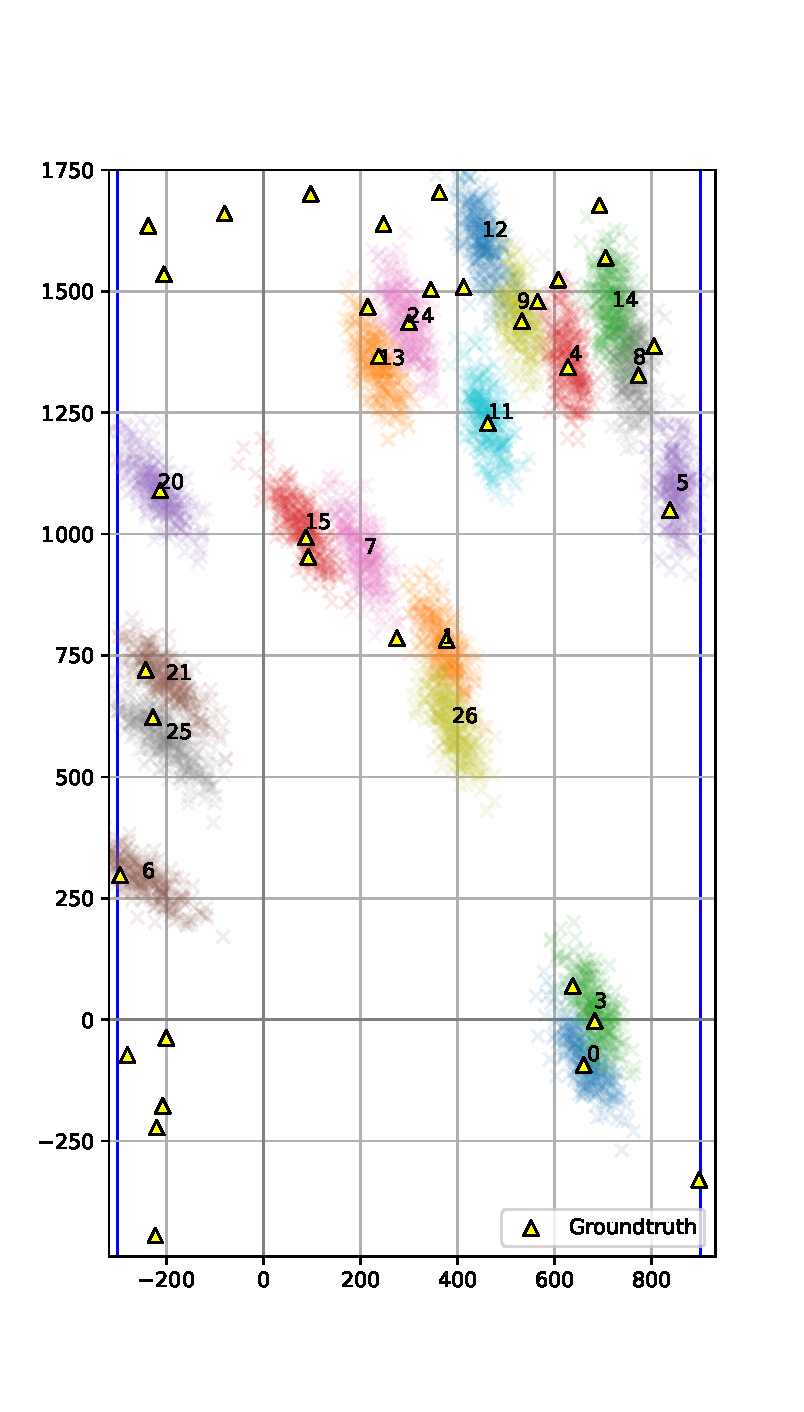
\includegraphics[width=0.4\linewidth]{oneCam_gaussian.png}
%   \caption{单个摄像头二维高斯概率分布建模}
%   \label{oneCam_gaussian}
% \end{figure}
对于WildTrack数据集,将七个摄像头所得行人在地面上的足点进行二维高斯概率分布建模后,投影在同一张图上,如图~\ref{b}所示,其中黄色三角为真实标注点,相同颜色的椭圆为同一摄像头来源的二维高斯概率分布建模。
% \begin{figure}
%   \centering
%   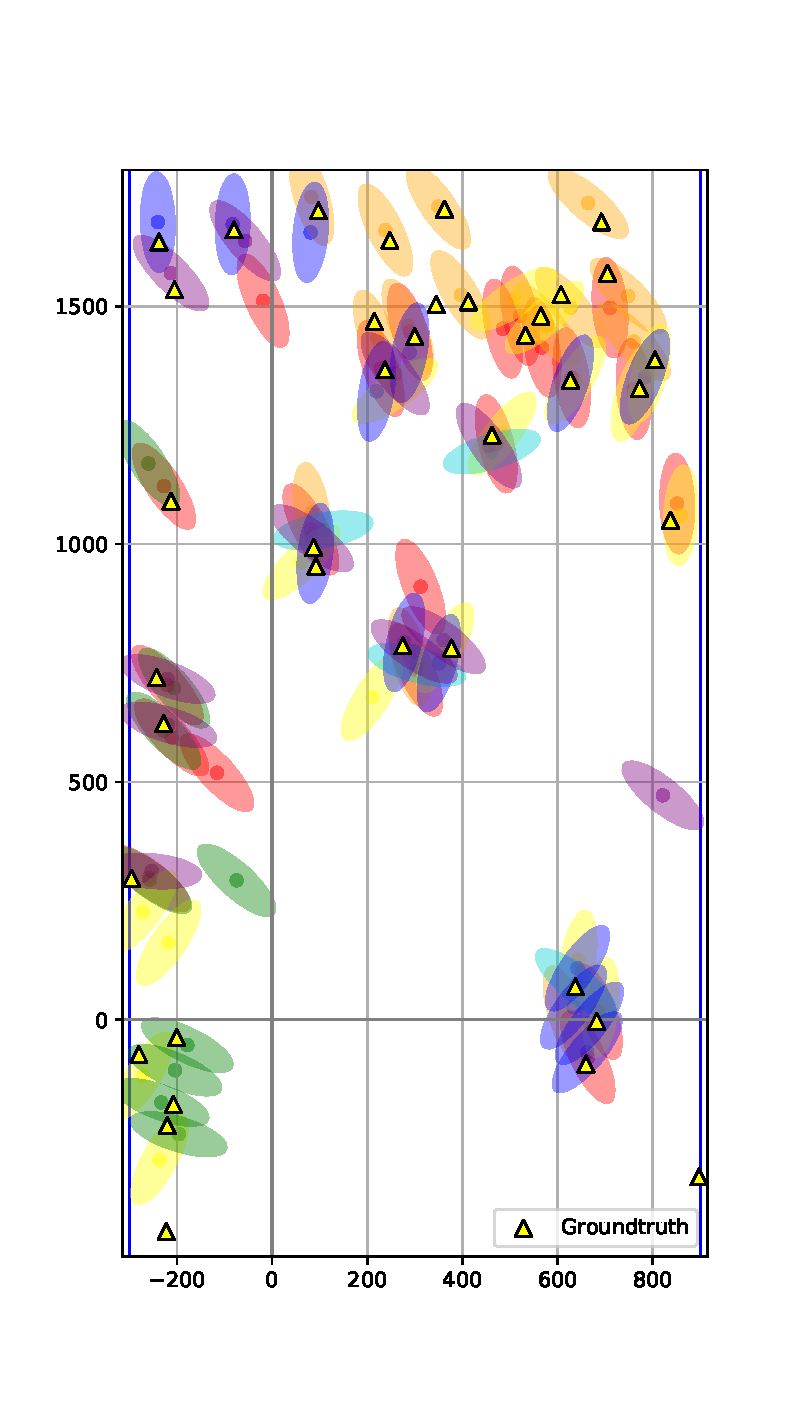
\includegraphics[width=0.35\linewidth]{multi-cam_gaussian.pdf}
%   \caption{单个摄像头二维高斯概率分布建模}
%   \label{multiCam_gaussian}
% \end{figure}
\begin{figure}
  \centering
  \subcaptionbox{\label{a}}
    {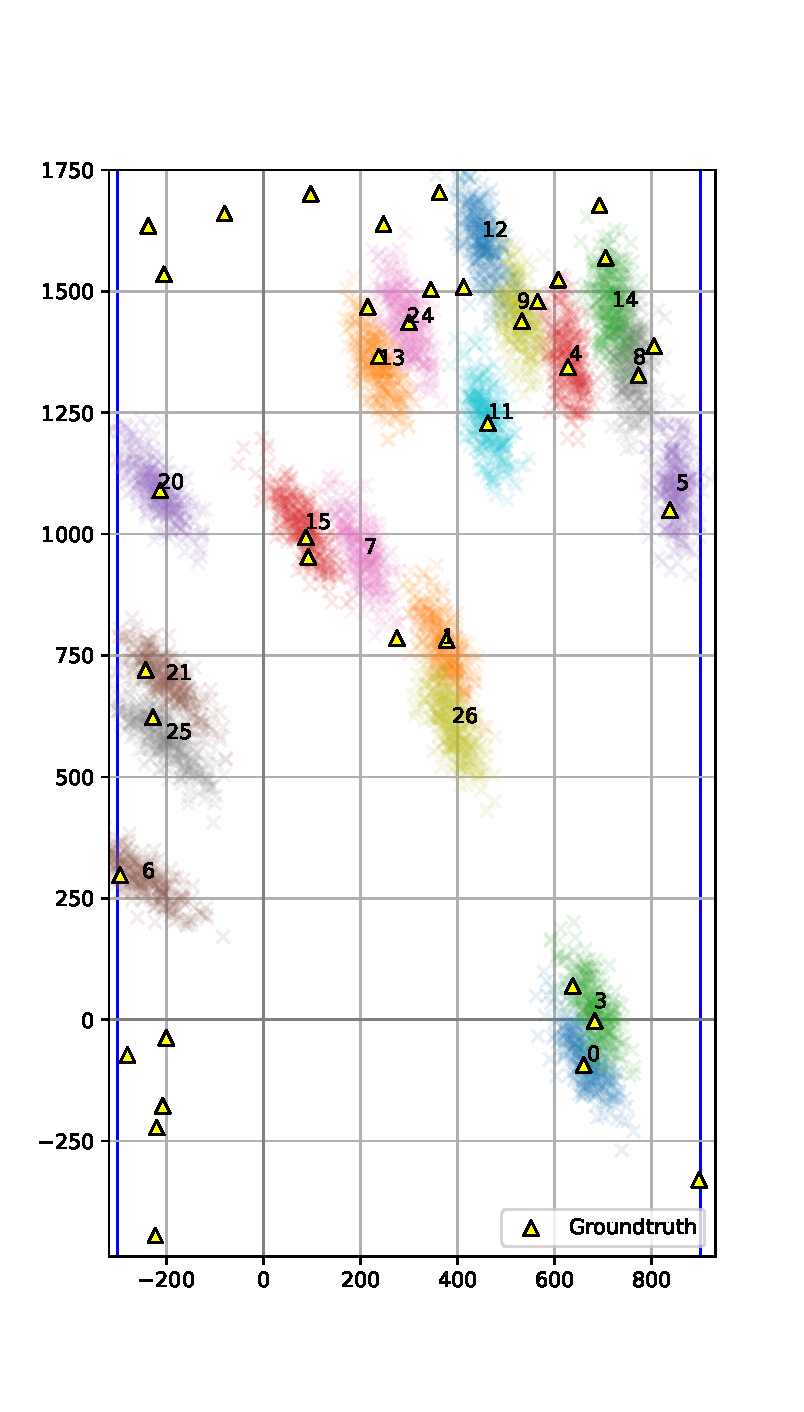
\includegraphics[width=0.4\linewidth]{oneCam_gaussian.pdf}}
  \subcaptionbox{\label{b}}
    {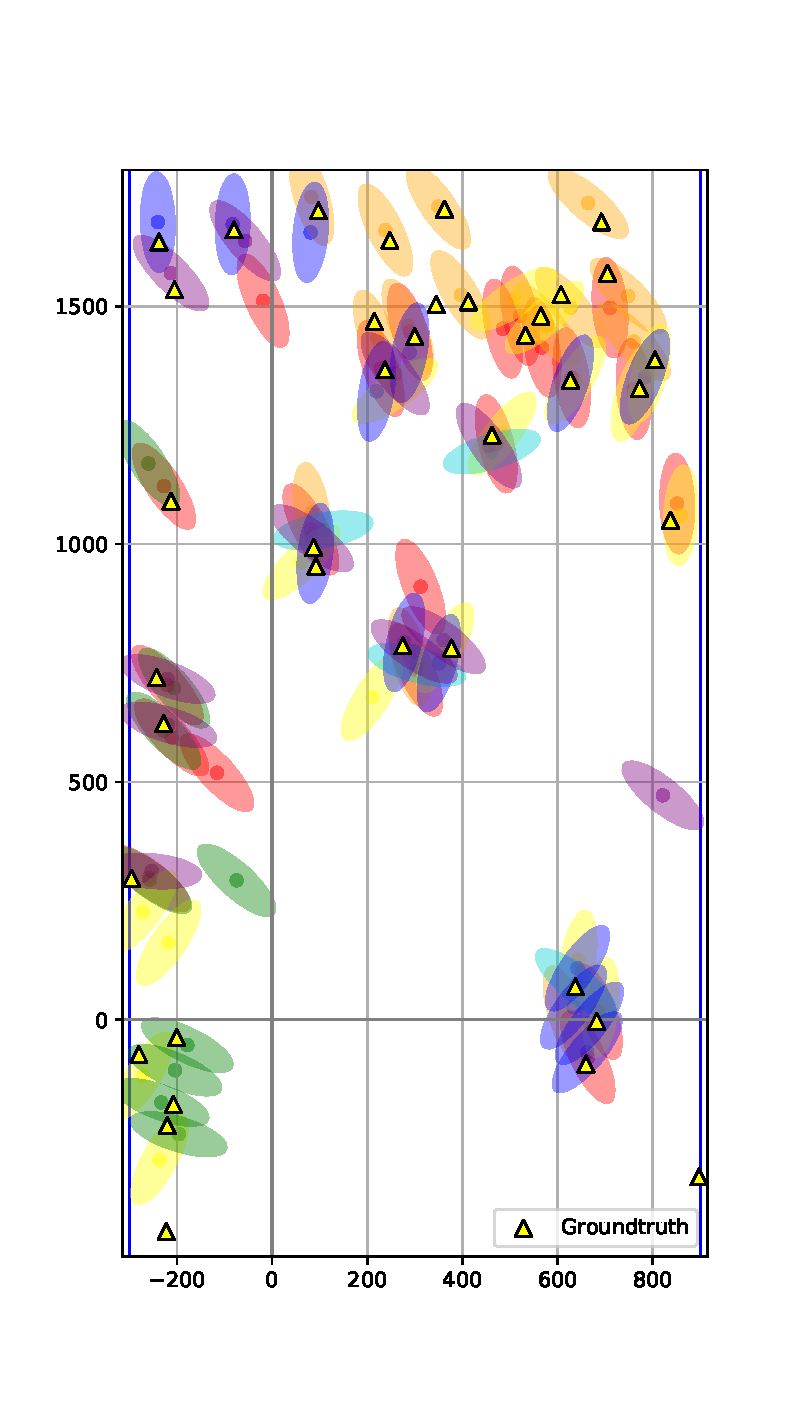
\includegraphics[width=0.4\linewidth]{multi-cam_gaussian.pdf}}
  \caption{多个分图的示例}
  \label{gaussian}
\end{figure}


\section{本章小结}

本章主要内容为深度学习算法的前置步骤。首先介绍了数据集的扩充和预处理过程,然后说明了所使用的现成行人检测算法的选取和具体实现细节,之后比较详细地介绍了相机投影原理和如何利用相机投影对得到的行人姿态节点进行处理,从而计算出行人的实际地面位置坐标,最后,详细介绍了所采用的二维高斯概率分布建模原理,阐明了所得行人地面位置坐标和相机参数如何决定了高斯概率分布的参数。这些步骤,为后续的数据融合和深度学习算法的使用做了铺垫。
% !TeX root = ../thuthesis-example.tex

\chapter{数据准备与深度学习方法构建}

上一章中,我们对行人在实际地面的位置进行了二维高斯概率分布建模,而在这一章中,我们将利用层次聚类的方法融合不同摄像头的数据,并利用深度学习网络对WildTrack数据集场景进行学习,最终得到更精确的行人位置估计结果。

\section{层次聚类方法}

在上文中的二维高斯概率分布建模中,对于每个行人每个摄像头的数据均进行了一次建模过程。因此,对于每个行人的位置,有来自多个摄像头的二维高斯概率分布来建模其在特定摄像机视角下的位置概率分布。于是,我们需要对每个行人将其来自多个摄像头的位置概率进行融合,最终可得到一个确定的预测点。以此点与真实地面坐标的差异为指标,可以反向优化前述二维高斯概率分布建模时和数据融合时的超参数。令预测点与真实地面坐标的差异趋于最小值,则可得到最优的超参数。利用此最优超参数生成后续神经网络输入的热图,可以最大化神经网络方法的效果。

本文中对于相同行人来自不同摄像头的二维高斯概率分布建模融合方式为层次聚类的方法,其优势主要是模型的解释能力比较强。层次聚类包含两种方式,即凝聚型层次聚类和分裂型层次聚类。本文中使用自下而上的凝聚型算法,其核心原理是:将每个二维高斯概率分布作为初始节点,初始假设每个节点都是一类,每一次迭代将会聚合最相近的两个点或聚类,当所有点或聚类都合并成一类或者满足停止条件时,则终止模型迭代,此时便得到了聚类结果。

在聚类过程中,我们采用了Alejandro López-Cifuentes\cite{A2018Semantic}等人提出的在融合地面点时的两个约束条件。即,属于同一个行人的所有二维高斯概率分布都需满足:
\begin{enumerate}
    \item 来自不同的摄像机(因为每帧中一个行人只可能出现一次);
    \item 二者之间距离必须低于阈值$t_{g}$。
\end{enumerate}
同时,在层次聚类时,计算两个组合数据点间距离的方法有三种,分别为Single-Linkage,Complete-Linkage和Average-Linkage。在选择合适的距离计算方法之前,我们先来介绍下这三种计算方法以及各自的优缺点。
\begin{itemize}
    \item Single-Linkage:将两个不同聚类的数据点中距离最近的两个数据点间的距离作为这两个聚类之间的距离。这种方法有一个缺陷,即容易受到极端值的影响。两个距离并不近的聚类,可能会因为其中两个极端点距离过近而融合,影响最终聚合效果;
    \item Average-Linkage:将两个不同聚类的数据点中距离最远的两个数据点间的距离作为这两个组合数据点的距离。这种方法的缺陷与Single-Linkage相反,即两个距离比较近的的聚类可能由于其中的极端值距离较远而无法聚类;
    \item Complete-Linkage:这种距离的计算方法是计算两个聚类的每个数据点与其他所有数据点的距离,将所有距离均值作为两个聚类间距离。这种方法计算量比较大,但结果比前两种方法更合理。
\end{itemize}
因此,本文层次聚类中选择了更合理的Complete-Linkage。同时,二维高斯概率分布之间的距离若直接用中心点之间的距离来衡量,则会损失其所估计的位置概率信息,于是本文采用相对熵(Relative Entropy),又被称为KL散度(Kullback-Leibler Divergence),来度量两个概率分布(Probability Distribution)间差异。在信息理论中,相对熵等价于两个概率分布的信息熵(Shannon Entropy)的差值。设$P(x), Q(x)$是随机变量$X$上的两个概率分布,在连续随机变量的情形下,相对熵的定义为:
$$
\text{KL}(P\|Q)=\int P(x)log{\frac{P(x)}{Q(x)}}dx
$$
但由于此处所有概率分布均为二维高斯概率分布,故它们之间的KL散度可以方便地用下式来计算:
$$
\begin{aligned}
\text{KL}&\left(N(x|\bm{\mu_1},\Sigma_1)|N(x|\bm{\mu_2},\Sigma_2)\right) \\
&=\frac{1}{2}\left[log{\frac{|\Sigma_2|}{|\Sigma_1|}}-K+tr(\Sigma_2^{-1}\Sigma_1)+(\bm{\mu_1}-\bm{\mu_2})^\top\Sigma_2^{-1}(\bm{\mu_1}-\bm{\mu_2})\right]
\end{aligned}
$$
其中,$N(x|\bm{\mu_1},\Sigma_1)$为$\bm{\mu}=\mu_1, \Sigma=\Sigma_1$的二维高斯概率分布,$N(x|\bm{\bm{\mu_2}},\Sigma_2)$为$\bm{\mu}=\bm{\mu_2}, \Sigma=\Sigma_2$的二维高斯概率分布。最后,得到层次聚类结果后,由于相机有重叠的视野,所以我们丢弃只有一个数据点的聚类,从而减少了错误聚类的数量,提升了聚类效果。最终得到的层次聚类结果如图~\ref{HC_a}所示,其中黄色三角形为行人实际地面位置,而橙色星形为层次聚类得到的行人地面位置估计。作为补充,图~\ref{HC_b}中也显示了作为层次聚类输入的人物位置二维高斯概率分布(以椭圆形表示),其中来自同一摄像头的分布用同一种颜色表示,同一颜色、同一序号的二维高斯概率分布为同一聚类。
\begin{figure}
    \centering
    \subcaptionbox{\label{HC_a}}
      {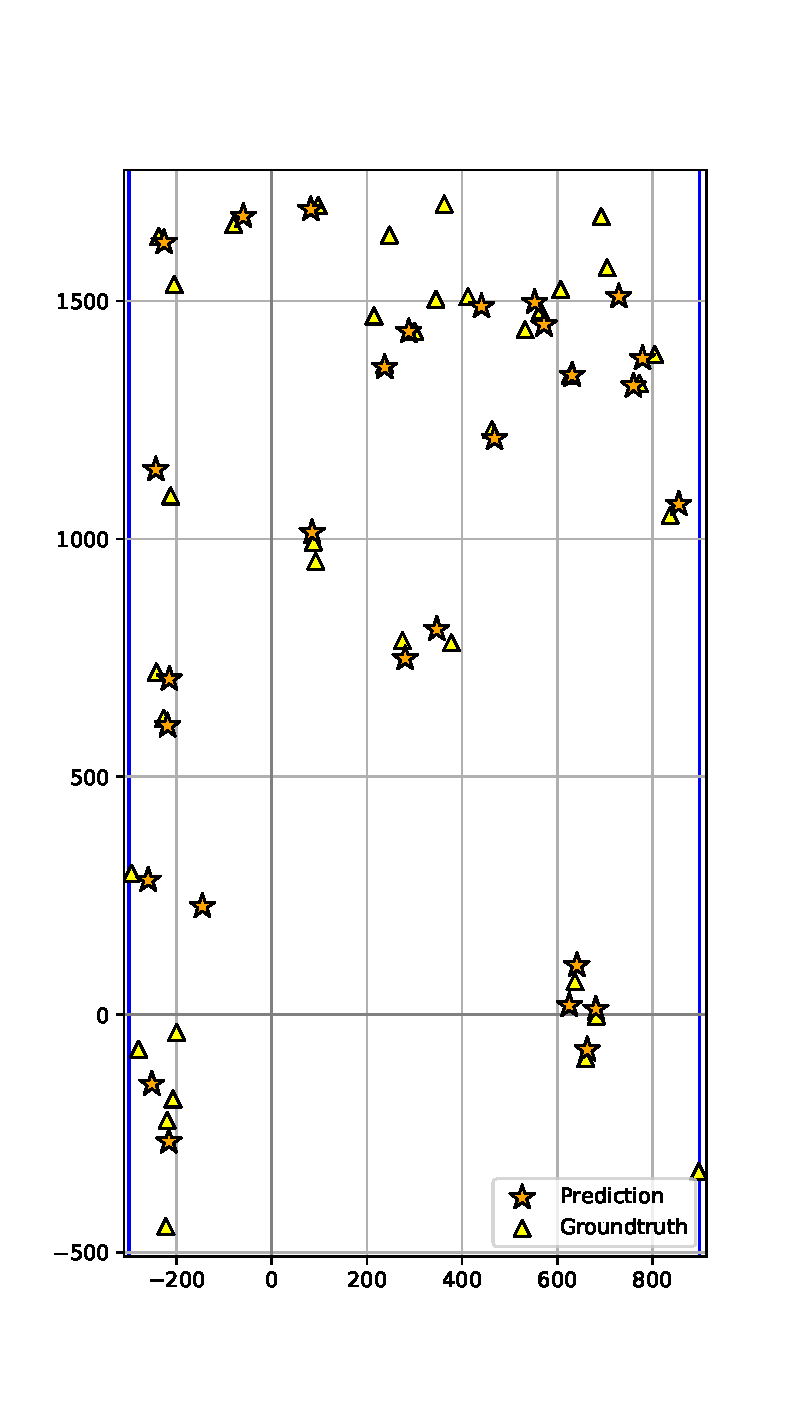
\includegraphics[width=0.4\linewidth]{HC.pdf}}
    \subcaptionbox{\label{HC_b}}
      {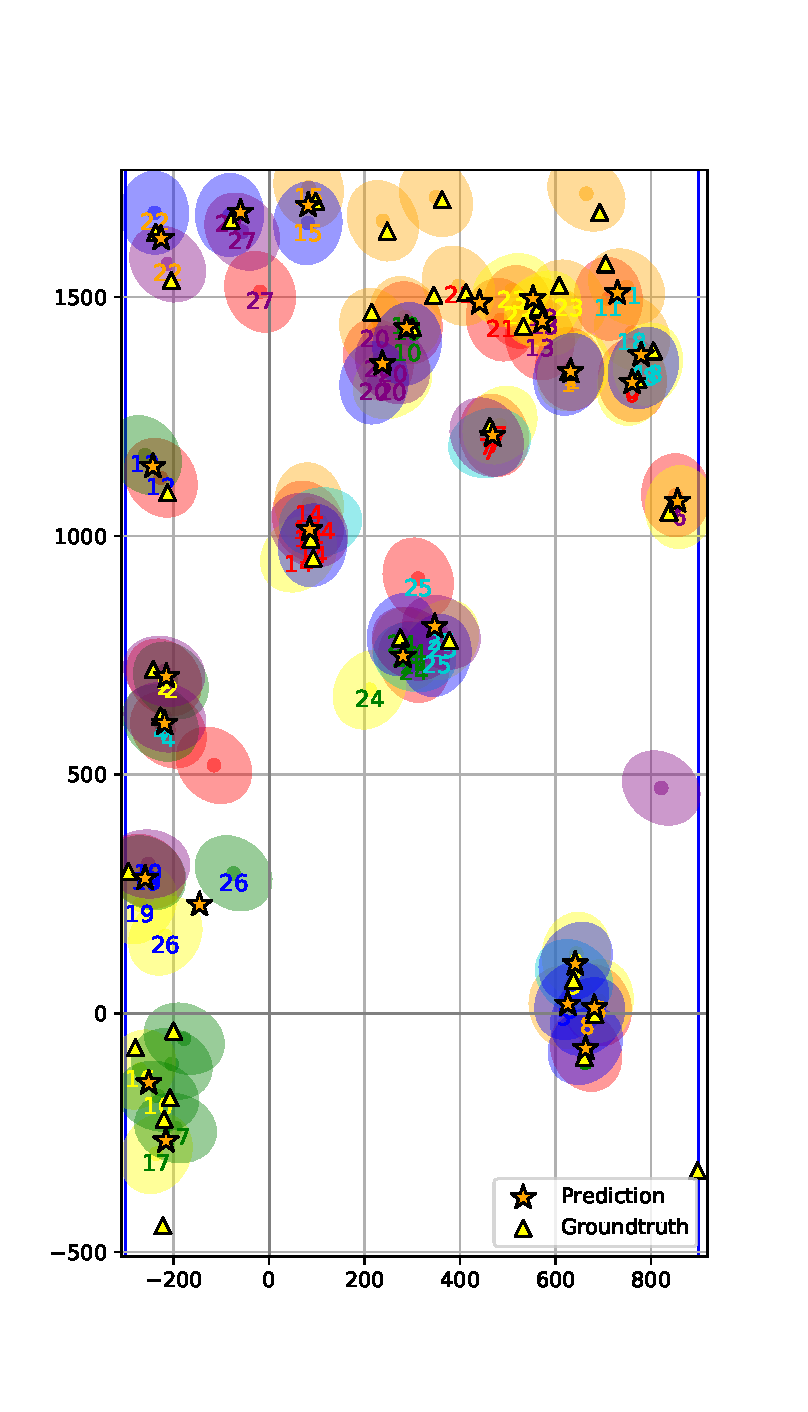
\includegraphics[width=0.4\linewidth]{HC_gaussian.pdf}}
    \caption{层次聚类结果}
    \label{HC}
\end{figure}

\section{深度学习数据准备}

对二维高斯概率分布进行聚类融合之后,接下来需要生成适用于后续神经网络输入和输出的图片。对于输入,本文将前述得到的二维高斯概率分布投影到一张大小为$224\times672$的热图(Heatmap)中,便于神经网络处理。为了得到最优的热图,需要对前述生成二维高斯概率分布的超参数进行调整。调整的方法是,令层次聚类得到的聚类中心点与真实地面坐标的差异趋于最小值,在此过程中进行参数记录,则可得到最优的超参数如下表~\ref{parameter_table}所示。利用此最优超参数生成后续神经网络输入的热图,可以最大化神经网络方法的效果。

接下来,使用上述参数得到二维高斯概率分布后,将其投影到热图中。而输入神经网络中的真值标签图,则可以使用真实地面坐标的占据图(Occupancy Map)\cite{fleuret2007multicamera}表示。最终所得热图如图~\ref{heatmap}所示,标签图如~\ref{occupancyMap}所示。

最后,在输入神经网络前,还需要划分数据集。本文将上文中数据集扩充时通过提取的视频帧作为训练集,将官方提供的400帧图片集作为测试集。
\begin{table}
    \centering
    \caption{反向优化得到的最优超参数}
    \begin{tabular}{lll}
        \toprule
        参数 & 值  & 描述         \\
        \midrule
        $k_{c}$ & 700 & 二维高斯概率分布中$C=k_{c}\bm{v}^\top\bm{v}, C'=k_{c}\bm{v}'^\top\bm{v}'$中的$k_{c}$ \\
        $k$   & 0.85 &  二维高斯概率分布中$\Sigma=kC + (1-k)C'$中的$k$   \\
        $t_{g}$ & 19cm &  层次聚类中聚为一类的阈值距离  \\
        $t_{ankle}$ & 0.35 &  单目探测器结果中保留概率超过$t_{ankle}$的脚踝节点 \\
        \bottomrule
    \end{tabular}
    \label{parameter_table}
\end{table}

\begin{figure}
    \centering
    \subcaptionbox{热图\label{heatmap}}
      {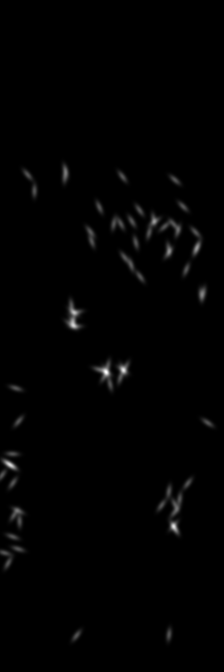
\includegraphics[width=0.2\linewidth]{frame1_heatmap.png}}
      \quad
    \subcaptionbox{标签图\label{occupancyMap}}
      {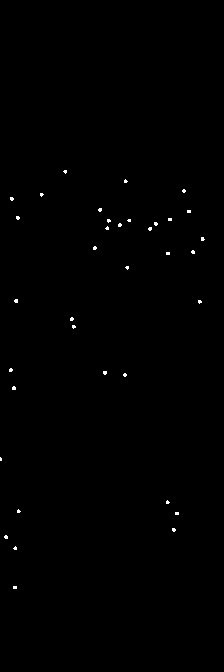
\includegraphics[width=0.2\linewidth]{frame1_occupancyMap.png}}
    \caption{神经网络输入与标签}
    \label{inputs_outputs}
\end{figure}



\section{深度学习神经网络}

\subsection{神经网络选择}

现在,我们的目标是利用深度学习算法对输入的位置概率特征进行学习,最终得到能够准确得到行人的位置。具体来说,即输入高斯概率分布热图,输出对应行人位置的占据图(Occupancy Map)。目前,在图像分析领域,深度学习方法实现的语义分割取得了很大的进展\cite{2016V, 2015U, 2017Road},本文也拓展了语义分割在行人位置估计上的应用。在生物医学应用的语义分割领域,一种流行的深度学习体系结构是U-Net\cite{2015U},它在2015年ISBI细胞跟踪挑战上达到了最好的性能,而ResUNet(Residual U-Net)\cite{2017Road}结构作为U-Net结构的改进,在道路图像提取中达到了最优的性能。同时,ResUNet++\cite{2019ResUNet}以ResUNet为基础发展而来,在医学图像分割领域取得了很不错的效果。本文基于以上进展,将上述网络作为本文工作的基础,实现了ResUNet和ResUNet++两种架构,将其作为多摄像头多目标行人位置估计的深度学习方法部分。

\subsection{神经网络结构}

本文所实现的ResUNet使用了U-Net、残差块等结构(Residual Units),而ResUNet++则在ResUNet的基础上加入了挤压和激励单元(Squeeze and Excitation Units)、空洞空间金字塔池化(Atrous Spatial Pyramid Pooling, ASPP)和注意力机制(Attention Units),从而提升了效果。下文对这些结构一一介绍,并阐明其在网络中的作用。

U-Net:在语义分割中,为了获得更好效果,在保留高级语义信息的同时必须使用低级信息细节。然而,训练这样一个深度的神经网络是很困难的,尤其是当训练样本很有限时。解决此问题的一种方法是Long等人\cite{2015Fully}提出的先使用预训练的网络,然后在目标数据集上对其进行微调。而另一种方法则是采用U-Net\cite{2015U}中使用的数据扩充方法。此外,U-Net的体系结构也有助于缓解训练的困难,这是因为将低级特征复制到相应的高级特征上,实际上创建了一条信息传播路径,允许信号更容易地在低级和高级特征之间传播。这样不仅有助于训练的反向传播过程,而且还可以将低级特种中的细节补偿到高级语义特征上去。这种特点和ResNet\cite{he2016deep}中提出的的Residual Units原理很相似。可见,U-Net结构是一种适合本文中最后部分位置估计的网络基础结构。

残差块(Residual Units):在ResNet网络提出之前,传统的卷积神经网络都是通过将一系列卷积层与池化层进行堆叠得到的。一般认为,网络越深,特征信息越丰富,模型效果应该越好。但是实验证明,效果并非如此。这是因为当网络深度堆叠到一定程度时,会发生梯度消失或梯度爆炸的问题和退化问题(Degradation Problem)\cite{he2016deep}。因此,何凯明等人提出了残差块来解决此问题。残差块的功能可由下式表示:
\begin{equation*}
    \begin{split}
    \mathbf{y}_{l}\ \ \ & = h(\mathbf{x}_{l})+\mathcal{F}(\mathbf{x}_{l}, \mathcal{W}_{l}), \\
    \mathbf{x}_{l+1} & = f(\mathbf{y}_{l}),
    \end{split}
\end{equation*}
其中,$\mathbf{x}_{l}$和$\mathbf{x}_{l+1}$是第$l$个残差单元的输入和预测,$\mathcal{F}(\cdot)$为残差函数,$f(\mathbf{y}_l)$是激活函数,$h(\mathbf{x}_{l})$是恒等映射函数,例如$h(\mathbf{x}_{l}) = \mathbf{x}_{l}$这样的函数就是恒等映射函数。在一个残差块中,有以不同方式组合的批标准化(Batch Normalization),ReLU激活函数和卷积层,而本文中采用了何凯明\cite{he2016deep}提出的综合性能最好的组合方式,图~\ref{residual_compare}展示了未采用残差块与采用残差块的对比,同时展示了所采用残差块的结构。
\begin{figure}
    \centering
    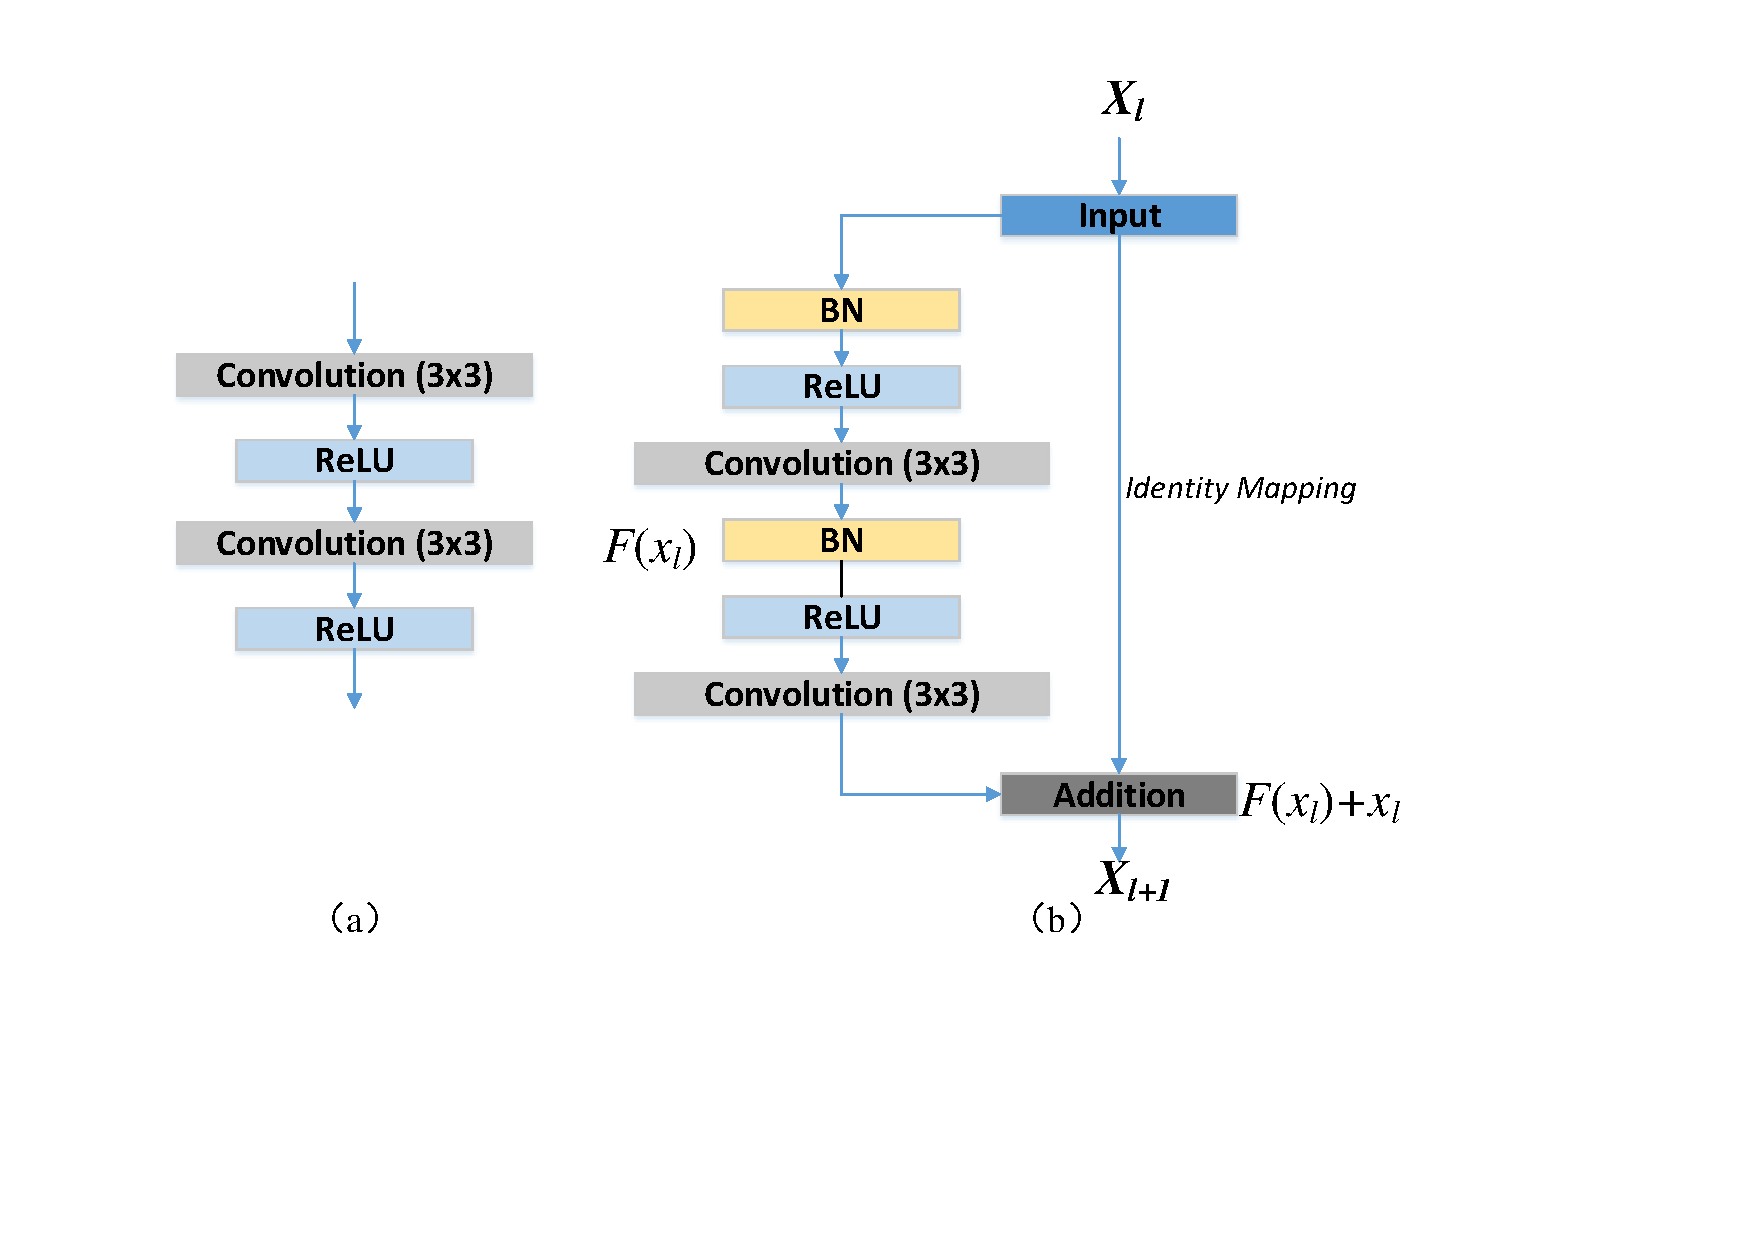
\includegraphics[width=0.5\linewidth]{res-u-net-blocks.pdf}
    \caption{(a)未采用残差块与(b)采用残差块的对比}
    \label{residual_compare}
\end{figure}

ResUNet:结合上述U-Net和残差块的技术,可以构建ResUNet网络\cite{2017Road}。这种结合可以带来两个优势:1)残差块使得可以构建的网络深度大大增加;2)残差块内部和网络高、底层次之间的直接连接大大减少了信息传播中的退化现象,从而在提高效果的同时还可以减少网络参数。本文所实现的ResUNet网络结构如图~\ref{Net_a}所示。网络采用了七层结构,为自编码器结构,主要分为编码层、中间层和解码层。编码层将输入的图片编码为压缩抽象表示,而解码层将压缩抽象表示解码为与输入大小相同的输出图片,中间层主要起到连接编码层和解码层、传输特征的作用。
\begin{figure}
    \centering
    \subcaptionbox{ResUNet网络结构\label{Net_a}}
      {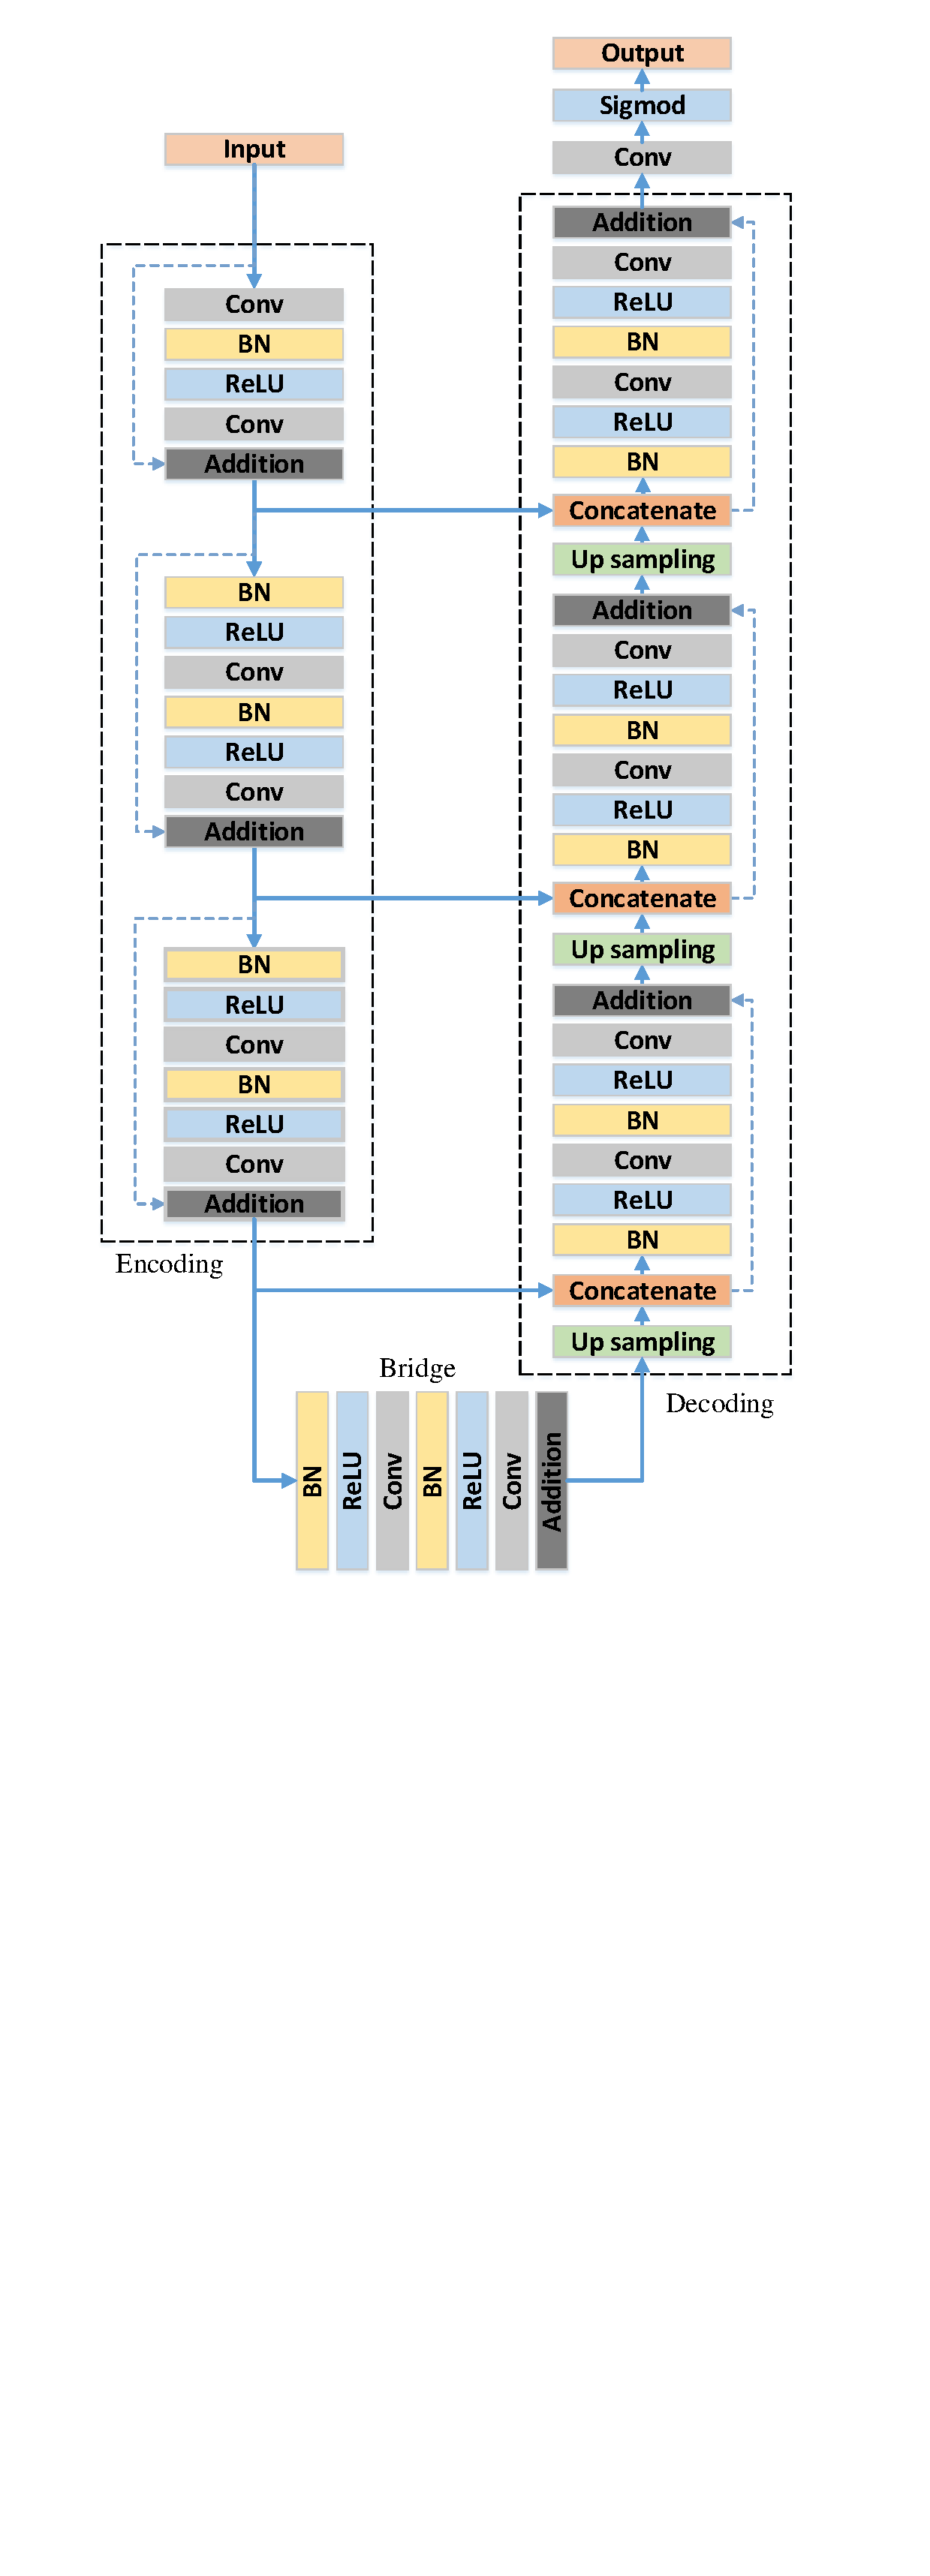
\includegraphics[width=0.36\linewidth]{ResUNet.pdf}}
    \subcaptionbox{ResUNet++网络结构\label{Net_b}}
      {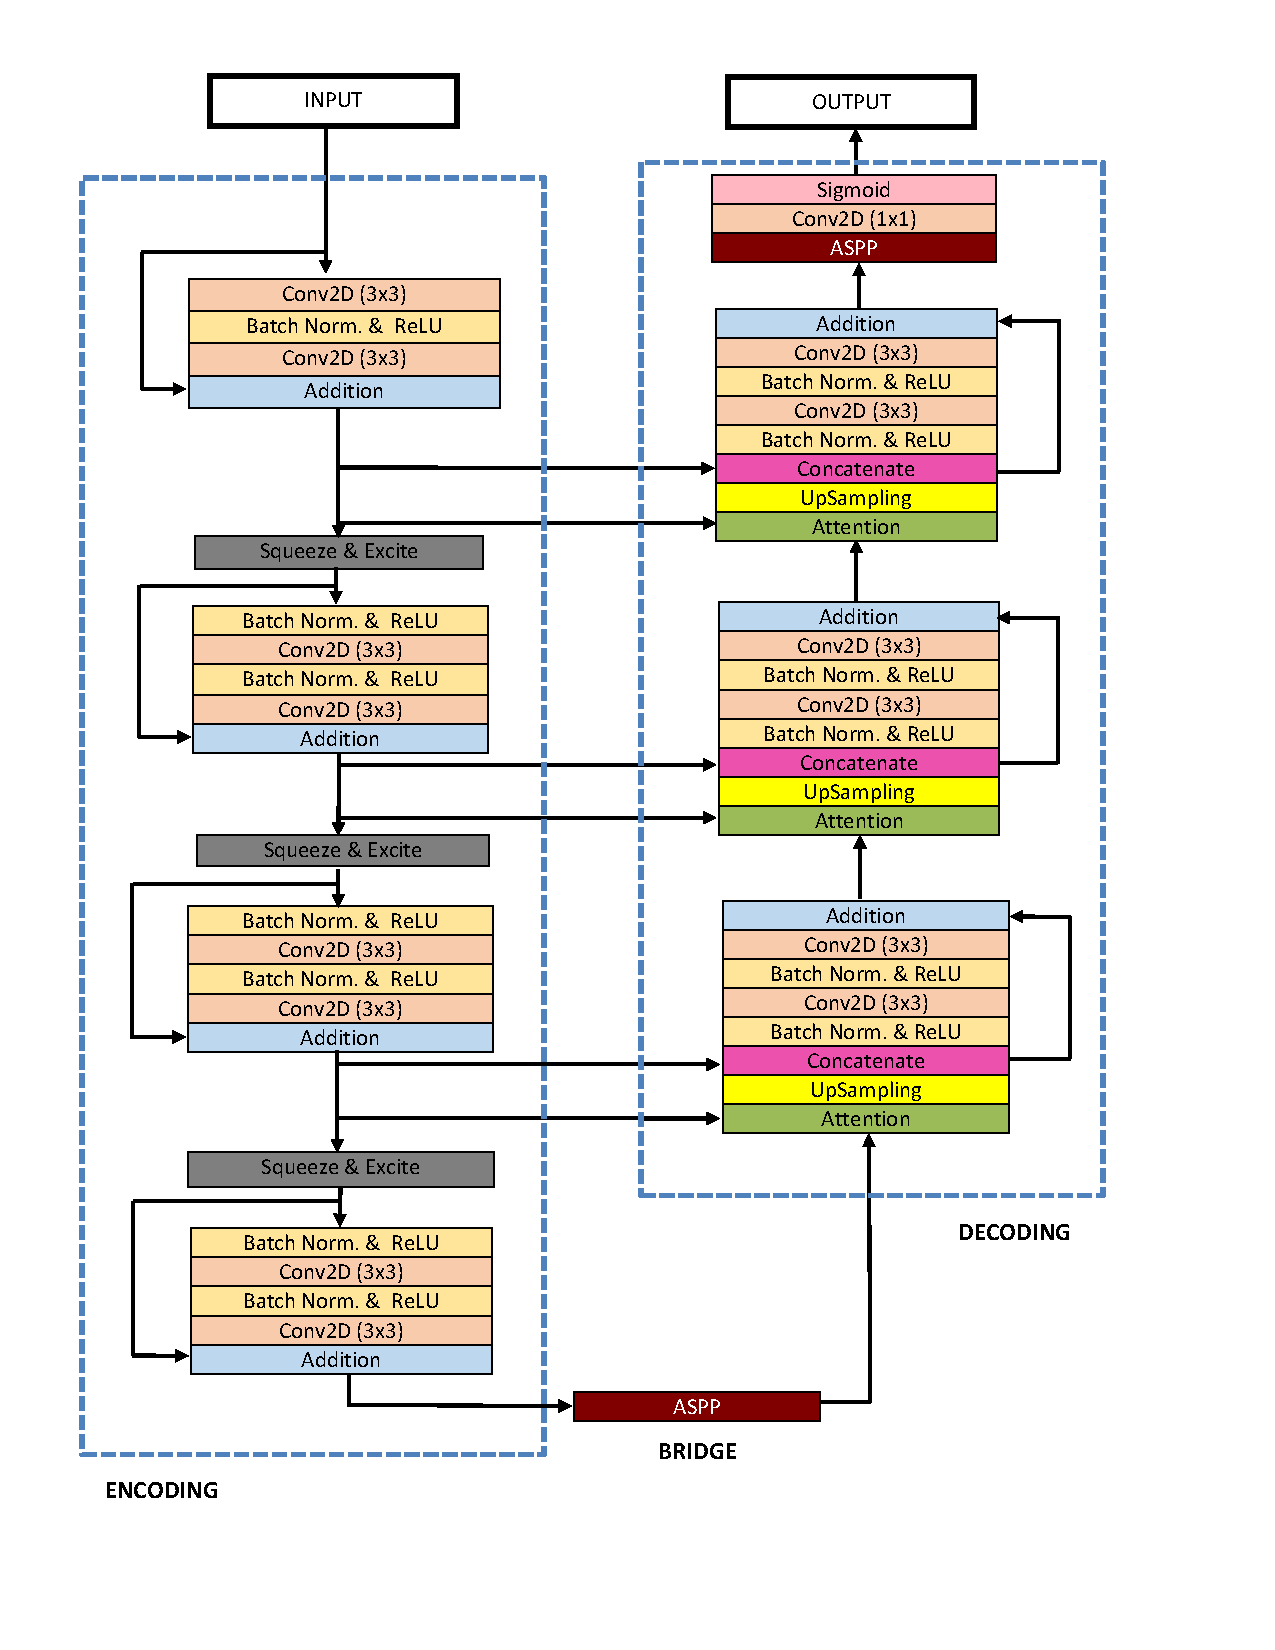
\includegraphics[width=0.62\linewidth]{ResUNet++.pdf}}
    \caption{本文实现的两种神经网络结构}
    \label{Net}
\end{figure}

挤压和激励单元(Squeeze and Excitation Units):挤压和激励网络(Squeeze-and-Excitation Networks)\cite{2017Squeeze}通过精确建模网络中通道的相互依赖关系,以及校准特征的方法,大大提高了网络的表示性能。因此,本文所采用的ResUNet++中也使用了挤压和激励单元,其主要目的是提高网络对关注特征的敏感性,抑制不必要特征。正如其名,挤压和激励单元实施的操作为先挤压全局信息并通过全局平均池(Global Average Pooling)来生成信息,然后激励以得到通道之间的相关性。

空洞空间金字塔池化(Atrous Spatial Pyramid Pooling, ASPP):何凯明等人\cite{2014Spatial}提出的ASPP方法,使得网络可以控制视野从而精确捕获多个尺度的信息。在本文实现的ResUNet++中,ASPP主要作为编码器和解码器之间的中间层,其作用主要是为语义分割提取多尺度的信息。

注意力机制(Attention Units):注意力机制实质上是一种分配机制,其核心思想是突出对象的某些重要特征,使得网络能够根据对象的重要程度重新分配资源。注意力机制的主要优势是可以被简单地运用在任何尺寸的输入中,显著提升特征的质量,从而促进效果的提升。在本文实现的ResUNet++中,注意力机制被加入到解码器的部分,从而使得网络能够专注于特征图中的关键区域。

ResUNet++:结合上述挤压和激励单元、空洞空间金字塔池化和注意力机制,在ResUNet的基础上,本文实现了ResUNet++网络。网络也分为七层结构,与ResUNet的结构基本一致,但加入了挤压和激励单元、空洞空间金字塔池化和注意力机制,从而大大提升了网络的预测效果。

\subsection{损失函数}

在构建的ResUNet和ResUNet++两个深度学习神经网络中,本文均采用了二进制交叉熵(Binary Cross Entropy, BCE)损失和Dice系数(Dice Coefficient)损失相结合的损失函数。二进制交叉熵可由下式计算:
\begin{equation*}
  \mathcal{L}_{BCE} = \frac{1}{N}\sum_{n=1}^{N}l_{n}
\end{equation*}
其中,$l_n=-w[y_n \cdot log{x_n}+(1-y_n) \cdot log(1-x_n)]$为第$n$个样本对应的loss,其中$w$为超参数。在本文中,上式loss体现为将预测图的第n个像素作为样本,标签图的第n个像素作为样本标签的loss。而Dice系数是一种集合相似度度量函数,通常用于计算两个样本的相似度。Dice系数损失的计算可由下式得到:
\begin{equation*}
  \mathcal{L}_{Dice} = 1-\frac{2|X \cap Y|}{|X|+|Y|}
\end{equation*}
其中,$X$为预测图,$Y$为标签图,$|X \cap Y|$是$X$和$Y$之间的交集,$|X|$和$|Y|$表示$X$和$Y$的元素的个数。在实际计算时,$|X \cap Y|$近似为预测图和标签图之间的点乘,并将点乘的元素的结果逐元素相加。而计算$|X|$和$|Y|$时,本文采取了直接进行逐元素相加的方式。

最终,将两种损失结合起来,就得到了本文所采用的损失函数,如下:
\begin{equation*}
  \mathcal{L} = \mathcal{L}_{BCE} + \mathcal{L}_{Dice}
\end{equation*}

\section{本章小结}

本章中介绍了构建层次聚类方法得到粗略的行人位置估计和通过粗略的估计结果反向优化高斯概率分布和层次聚类的超参数的过程,然后介绍了利用扩充和预处理后得到的数据如何被用来制作适合网络输入的热图和标签图。最后,详细阐述了本文所实现的ResUNet和ResUNet++两种深度学习神经网络结构和所采用的损失函数。这两种深度学习方法将输出行人位置估计的更准确的预测,可以作为本文工作中的估计结果。
% !TeX root = ../thuthesis-example.tex

\chapter{评价指标与实验结果}

本章首先介绍本文所实现的多摄像头多目标行人位置估计算法中所采用的实验评价指标,然后详细阐述实验过程和实验的环境、参数。最后,将实验结果与目前业界最新算法进行比较,并提出未来可能的改进建议。

\section{评价指标}

精确率(Precision)和召回率(Recall)是信息检索和统计学分类领域的两个应用很广泛的度量,用来评价结果的质量。本文采用了精确率、召回率来衡量最终位置估计效果。然而,由于在大规模数据集合中,精确率和召回率两个指标往往是相互制约的,因此,本文还采用了F分数(F-score)来综合权衡精确率和召回率。即,本文共使用了精确率、召回率和F分数三个评价指标来衡量最终的位置估计效果。

为了得到上述三个评价指标,首先需要得到实验结果的混淆矩阵(Confusion Matrix)。混淆矩阵也称误差矩阵,在本文中为两行两列的矩阵形式,其主要参数有四个,即真阳性(True Positives, TP)、真阴性(True Negatives, TN)、假阳性(False Positives, FP)、假阴性(False Negatives, FN)。在本文实验中,TP集合为与实际位置相符的预测点;TN集合应为预测点之外的点中排除实际位置的点,由于计算上述三个评价指标并没有用到TN集合,故被忽略;FP集合为预测点中没有命中实际位置的点;FN集合为没有被预测到的实际位置点。在本实验中,预测点与实际位置命中的判定半径为$r=0.5m$,即若预测点与实际点距离相聚小于50cm即判定为成功估计了行人的位置。

上文提到,计算混淆矩阵的参数时,需要判定预测点与实际位置点是否对应,从而判定是否正确预测。现在,我们得到了对行人位置在地面上的最终预测点,同时,我们有行人地面实际位置的标注,那么就需要将这些预测点和实际标注一一匹配起来,从而可以计算预测点与实际点之间的距离,以判断是否预测成功。解决上述匹配问题的方法可以抽象为图论中寻找最大匹配的算法,在本文中,上述问题抽象为在二分图中寻找最大匹配。因此,我们实现了匈牙利算法(Hungarian Algorithm)来解决这一问题。匈牙利算法利用深度优先搜索来不断寻找增广路。它从每个未匹配的实际地面点开始,如果直接找到了预测点中未匹配的点,则直接返回此匹配路径;若找到预测点已匹配的点,那么从该点匹配的点出发继续深度优先搜索未匹配点。

得到混淆矩阵后,可以计算上述三个评价指标。
\begin{itemize}
    \item 精确率(Precision) 精确率是针对预测结果而言的,它表示的是预测点中有多少是预测正确的。精确率显示了模型预测点的精确性,可由下式计算:
        \begin{equation}
            \text{Precision}=\frac{\text{TP}}{\text{TP}+\text{FP}}
        \end{equation}
    \item 召回率(Recall) 召回率是针对原来的样本而言的,它表示的是实际位置点中有多少被预测命中了。召回率显示了模型是否能够估计出视野中更多行人的实际位置,其可由下式计算:
    \begin{equation}
        \text{Recall}=\frac{\text{TP}}{\text{TP}+\text{FN}}
    \end{equation}
    \item F分数(F-score) 精确率和召回率指标有时候会出现矛盾的情况,这样就需要综合考虑二者,最常见的方法就是利用F分数,即精确率和召回率的加权调和平均:
    \begin{equation}
        \text{F-score}=(1+\beta^2)\cdot \frac{\text{Precision} \cdot \text{Recall}}{\beta^2 \cdot \text{Precision} \cdot \text{Recall}}
    \end{equation}
    本文中令$\beta=1$,即实际上使用F1-score。
\end{itemize}

\section{实验设置和结果分析}

我们利用了表~\ref{parameter_table}中的超参数进行层次聚类的数据融合,之后可以初步得到行人位置估计结果,这些实验结果与深度学习方法的比较如表~\ref{experiments}所示。

在深度学习方法中,主要在WildTrack数据集上进行实验。其中,作为训练集的是从WildTrack数据集提供的七个摄像头视频提取到的视频帧,每个摄像头共有11558张图片,其中真值由官方提供的400张图片真值插值得到;作为测试集的是WildTrack数据集提供的每个摄像头400张的去畸变图,提供了真值标注。实现的ResUNet和ResUNet++网络均基于PyTorch,部署在NVIDIA RTX 3090 GPU进行训练,系统版本为Ubuntu 18.04,提供CUDA 11.3支持。在训练的过程中,输入热图和输出预测图的尺寸均为$224\times 672$,输入网络时采用的Batch Size为4,使用Adam优化器进行调优。同时,为了避免网络难以收敛到最优状态,初始学习率设置为1e-3,每20个训练周期(epoch)学习率衰减为原来的0.1倍,一共训练100个周期。

将深度学习方法中ResUNet和ResUNet++网络的实验结果与目前领域内几个深度学习方法的比较如下表~\ref{experiments}所示。
\begin{table}
    \centering
    \caption{层次聚类方法、ResUNet和ResUNet++与其他方法实验效果比较}
    \begin{tabular}{llll}
        \toprule
        方法 & 精确率  & 召回率 & F分数                       \\
        \midrule
        Deep-Occlusion\cite{baque2017deep} & 95\% & 80\% & 86\%                  \\
        Generalized Mutiview Detection\cite{vora2021bringing} & 94\% & 93\% & 93\%  \\
        Hierarchical Clustering & 87\% & 62\% & 72\%         \\
        ResUNet & 92\% & 70\% & 79\%                         \\
        ResUNet++ & 95\% & 85\% & 90\%                      \\
        \bottomrule
    \end{tabular}
    \label{experiments}
\end{table}

由表~\ref{experiments}可以看出,ResUNet++网络结构效果比ResUNet效果好很多,而没有使用神经网络的层次聚类融合方法效果最差。同时,也可以发现,ResUNet++在多摄像头多目标行人位置估计领域,在未使用行人重识别和时序信息的情况下,达到了接近目前业界领先算法的效果。然而,我们可以发现几乎所有的结果中精确率都比召回率更高,尤其是ResUNet得到的结果。这是因为网络对输入的热图进行特征提取时,那些遮挡较少、有多个摄像头同时拍摄的行人会在热图中生成明显的概率分布聚集,从而提高了预测点的精确率。然而,在人员密集的区域,对行人的检测和估计难度迅速增大,从而导致了很多遮挡行人难以被检测到,因此导致预测点比实际点数量更少,从而降低了召回率。在本文提出的多摄像头行人位置估计算法中,关键的困难不是预测得到的位置点与实际点距离偏离过大,而是对于遮挡严重的行人,即使检测到其存在,也很难在多个摄像头中同时生成其二维高斯概率分布,导致生成的热图中遮挡严重的行人的特征比较混乱,因此容易被网络忽略和误判。因此,预测点将会比实际点少,从而导致召回率降低。

\begin{figure}
    \centering
      \subcaptionbox{输入热图\label{300heatmap}}
      {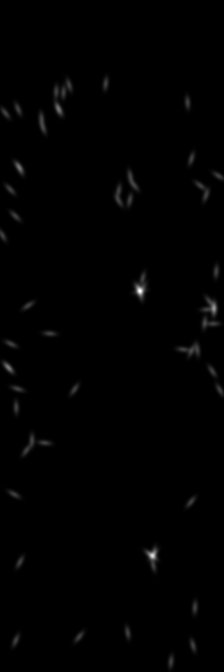
\includegraphics[width=0.2\linewidth]{000300_inputs.png}}
      \subcaptionbox{真值标签\label{300label}}
      {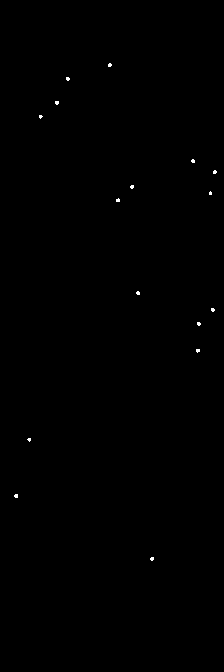
\includegraphics[width=0.2\linewidth]{000300_label.png}}
      \subcaptionbox{ResUNet++\label{300RPP}}
      {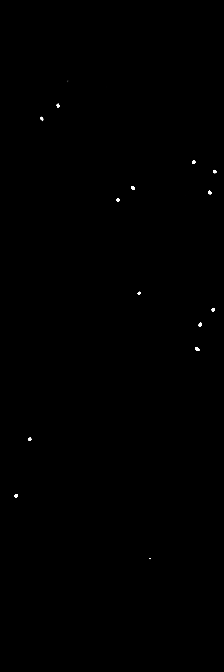
\includegraphics[width=0.2\linewidth]{000300_RPP.png}}
      \subcaptionbox{ResUNet\label{300R}}
      {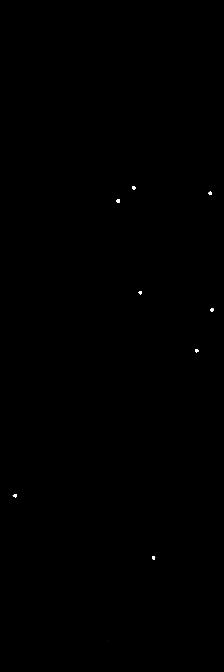
\includegraphics[width=0.2\linewidth]{000300_R.png}}
    \caption{预测结果示例1}
    \label{success}
\end{figure}

接下来,结合具体例子对估计结果进行分析。图~\ref{success}展示了一个位置估计相对比较成功的结果,在这一帧中,ResUNet++得到的结果精确度达到了100\%,召回率为94\%,F分数为97\%,而ResUNet得到的结果为精确度100\%,召回率为50\%,F分数为67\%。其中,预测比较成功的原因主要是当前图片内人物数量不多,互相遮挡的情况比较少,因而在第一步的AlphaPose姿态节点检测中就能得到比较准确的结果,得到的二维高斯概率分布图和生成的热图比较简单,同时,由于网络结构比较深入,对于这种相对简单的场景能够比较容易抓取其概率分布的特征,因此在ResUNet和ResUNet++中都取得了相对不错的效果。


然而,在图~\ref{failure1}中,可以看出预测的结果并不十分理想。在这一帧中,ResUNet++得到的精确度为92\%,召回率为58\%,F分数为71\%,而ResUNet为精确度为77\%,召回率为33\%,F分数为46\%,可见这一帧的预测过程中出现了很大障碍。从精确度和召回率相差很大的现象可以得出,在这一帧中最大的问题是有很多行人没有判断出来。出现这种现象是因为所采用的AlphaPose单目检测器,并不能直接输入高清图片,而是只能输入尺寸非常小的$256\times 192$的图片,在压缩尺寸的过程中自然丢弃了很多图像的内容信息。从图~\ref{failure1}中可以看到,ResUNet与ResUNet++都在左侧边缘区域以及左上角距离摄像头比较远的区域出现了很多未探测到行人的状况,印证了上述AlphaPose输入尺寸过小,导致较远处行人分辨率过低,难以辨认姿态节点,即使得到节点,其准确性也很差。针对此问题,未来可以将姿态估计部分改为输入高清图片,探测到行人后截取其检测框,然后将检测框输入网络判断姿态,便可完全利用摄像头捕捉到的行人外表信息,而不是现在将整幅图直接压缩尺寸后输入,造成信息损失。此外,在图中上侧的行人密集处,也出现了预测不全,这是因为此帧中行人密集处在不同摄像机视角下都有较多的遮挡,在这种复杂遮挡的背景下,不仅仅AlphaPose得到的姿态不准确,而且生成的二维高斯概率分布图也呈现出一种混乱的状况。针对这一问题,需要改进二维高斯概率分布建模过程。未来可以给每个二维高斯概率分布加入与摄像头距离相关的权重,或者让与摄像头的距离成为调节二维高斯概率分布大小和形状的重要因素,这样,可以将摄像头远近不同产生不同置信概率的信息加入到位置概率建模和热图生成过程中,如此可减少远处行人的概率分布混乱问题,同时增强近处行人的估计准确度。最后,左侧行人位置的估计不全还可能是因为左侧区域有一些行人在区域的边缘处,于是数据集的标注会呈现一定的不确定性,此外,此区域还有一些坐在台阶上的行人,这些行人在AlphaPose的探测中常常会被错误探测,从而造成了最终预测结果的失误。
\begin{figure}
    \centering
      \subcaptionbox{输入热图\label{045heatmap}}
      {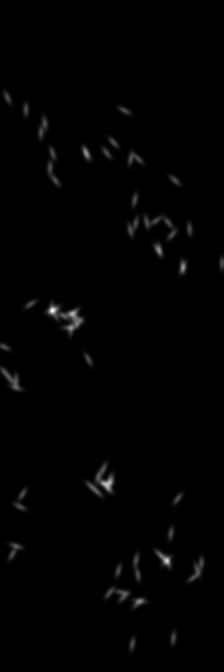
\includegraphics[width=0.2\linewidth]{000045_inputs.png}}
      \subcaptionbox{真值标签\label{045label}}
      {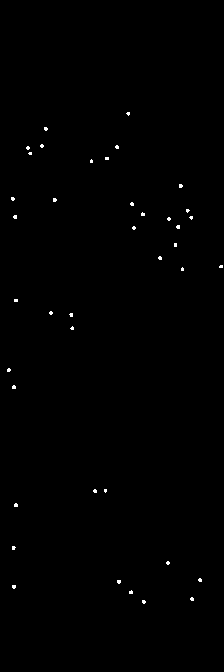
\includegraphics[width=0.2\linewidth]{000045_label.png}}
      \subcaptionbox{ResUNet++\label{045RPP}}
      {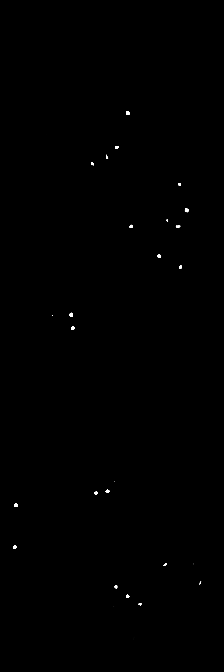
\includegraphics[width=0.2\linewidth]{000045_RPP.png}}
      \subcaptionbox{ResUNet\label{045R}}
      {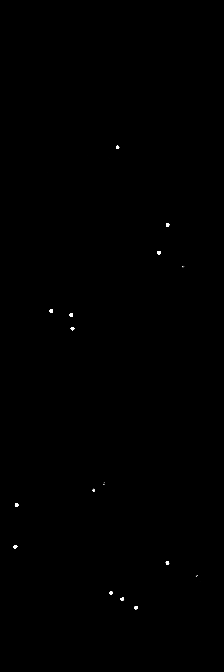
\includegraphics[width=0.2\linewidth]{000045_R.png}}
    \caption{预测结果示例2}
    \label{failure1}
\end{figure}

\begin{figure}
    \centering
      \subcaptionbox{输入热图\label{015heatmap}}
      {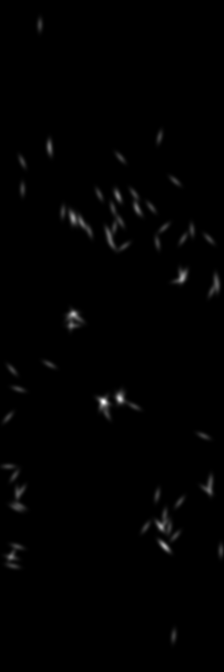
\includegraphics[width=0.2\linewidth]{000015_inputs.png}}
      \subcaptionbox{真值标签\label{015label}}
      {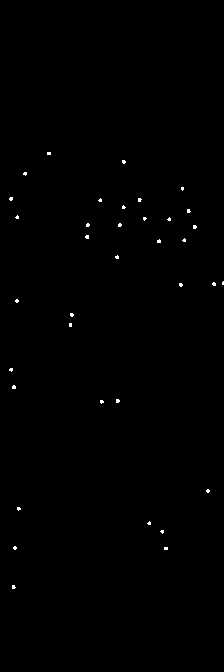
\includegraphics[width=0.2\linewidth]{000015_label.png}}
      \subcaptionbox{ResUNet++\label{015RPP}}
      {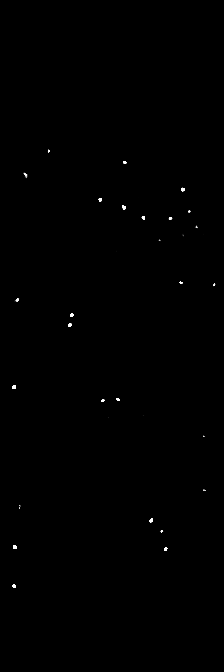
\includegraphics[width=0.2\linewidth]{000015_RPP.png}}
      \subcaptionbox{ResUNet\label{015R}}
      {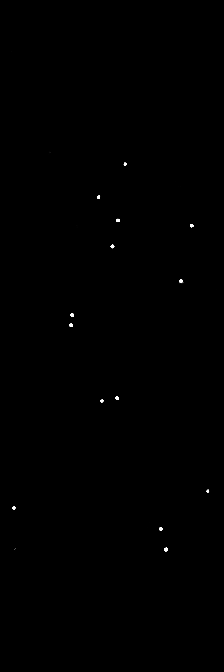
\includegraphics[width=0.2\linewidth]{000015_R.png}}
    \caption{预测结果示例3}
    \label{failure2}
\end{figure}

此外,在图~\ref{failure2}中,效果也不太理想,同时ResUNet++和ResUNet所得到的结果有较大的差异。在这一帧中,ResUNet++得到的精确度为97\%,召回率为75\%,F分数为84\%,而ResUNet为精确度为93\%,召回率为39\%,F分数为55\%。可见ResUNet的结果召回率相当低。在图中对比也可以发现,ResUNet++在人群密集区域有较多的未命中点,而ResUNet预测结果中有很多真实位置没有被估计到。ResUNet++在人群密集区域的缺陷上文已经举例分析,因此此处分析ResUNet与ResUNet++预测结果的差异。对比可见,在输入热图大块特征比较明显,即有多个摄像头同时拍摄到同一个行人的情况下,ResUNet++和ResUNet都呈现了不错的效果。但是在高斯概率分布相对混乱的区域,或者说,局部特征和纹理比较复杂的区域,ResUNet++取得了比ResUNet好得多的效果。这是因为ResUNet++加入的挤压和激励单元提高了网络对局部特征的敏感性,抑制了不必要的一些混乱的特征,同时空洞空间金字塔池化和注意力机制使得网络可以控制视野,专注于重要的局部特征,显著提升了特征的质量。因此ResUNet++相比ResUNet在概率分布比较混乱的部分能够取得更准确的结果。

最后,在层次聚类的反向调优过程中,可以通过设计更好的调优方法找到最佳的参数,从而得到更准确合理的热图,提高网络输出效果。此外,在将网络输出的预测图转变为实际位置时,也会产生一些误差,这些误差会对最终结果造成一定影响。

\section{本章小结}

本章中主要介绍了实验的评价指标、实验设置细节和具体实验结果的分析。实验的评价指标主要使用了精确率、召回率和F分数三个指标来衡量算法位置估计的效果,实验设置上,对数据集进行扩充以增加训练量,同时利用学习率衰减的训练策略,提升了训练效果。在实验结果方面,仅仅使用层次聚类来得到行人的位置估计的算法效果并不好,而在层次聚类的基础上利用ResUNet和ResUNet++的深度学习网络可以达到较好的效果。最后对实验结果进行分析,同时提出了一些未来改进的方向。所实现的ResUNet++在ResUNet基础上改进而来,达到了接近目前最优算法的性能。
% !TeX root = ../thuthesis-example.tex

\chapter{结论与展望}

\section{结论}

由于社会经济和科技的迅速发展,近年来摄像头在生活中已经越来越普遍。多摄像头行人位置估计是计算机视觉领域一个重要发展方向,今年来在人工智能和深度学习方法迅速发展的背景下取得了长足进步。在当今摄像头无处不在的背景下,多摄像头行人位置估计的应用场景也越来越多,社会对这项技术的需求也越来越大。这些行人位置估计算法的发展和成熟使得我们可以高效准确地在很多公共场所对行人进行跟踪或轨迹的预测,可以促进自动驾驶技术的进一步发展,甚至还可以应用于电影和游戏行业,促进虚拟现实技术的发展。可见,多摄像头行人位置估计算法很有研究的意义和价值。

本文所提出的多摄像头行人位置估计算法可以分为四个部分:行人检测、位置的相机投影与建模、数据关联和融合、特征学习与输出结果。其中行人检测直接使用即插即用的Alphapose中的预训练网络提取人体姿态节点,从而可以结合外观信息迅速得到行人的足点。此后,利用相机投影的原理将行人足点转为在实际地面上的二维高斯概率分布,从而巧妙地结合了不同视角的摄像机中不同行人位置不同的概率分布信息。在数据关联与融合阶段,利用KL散度作为距离,将地面上的行人二维高斯概率分布利用层次聚类的方式进行融合,再利用融合得到的粗略位置估计结果反向调整前面步骤的参数。这样,将不同视角摄像机的位置概率分布信息进行了很好的融合,有效地降低了遮挡带来的估计效果减退。最后,实现的ResUNet利用了U-Net和残差块的优势,在加深网络深度的同时减少了退化的现象。而在ResUNet基础上实现的ResUNet++则加入了挤压和激励单元、空洞空间金字塔池化和注意力机制,提高了网络的表示性能,同时使得网络能够控制视野、在更重要的特征上投入更多的关注度。ResUNet++在得到的二维高斯概率分布信息上训练,学习到了不同视角摄像机中的行人位置概率分布特征,提升了模型预测效果,接近业界先进水平。

\section{展望}

本文算法可以接近业界先进水平,但由于时间有限,未能继续在此算法中继续拓展和完善来推动其达到领先水平。在将来的工作中,我们还可以在以下方面作新的尝试,从而改进算法、提升效果。

首先,目前直接使用的Alphapose需要将高清摄像头输入压缩为$256\times 192$尺寸,因此在这个过程中损失了很多原有信息,未来可以先识别出人物得到其检测框后,将每个行人从高清图中截取下来,分别输入到姿态检测的神经网络中,这样便可以保留更多图像信息,提高每个人足点的预测精度。此外,当前算法,针对同一摄像机而言,行人与摄像机的距离远近对其二维高斯概率分布建模几乎没有影响,但众所周知,近处行人的位置概率分布区域显然应该比远处行人的概率分布更小,近处的行人应该有更精确的位置估计。因此,未来可以加入这一影响参数,也可以加入一个权重系数,使得距离摄像头更近的节点有更高的权重,从而提高位置估计精度。此外,本文算法对行人的外表特征并没有显式地利用,对于视频序列中的时序信息也未加以利用,未来可以加入行人重识别算法的部分功能,同时利用多个连续帧中同一行人位置变化连续的特点,进一步提升神经网络的预测效果。最后,还可以在网络的训练过程中利用数据集增强的方法,如裁剪、加入噪声等方法,进一步扩充数据集,以提高网络的适应性,另外,还可以加入权重衰减(Weight Decay)方法,尝试更多的训练策略,以使得网络发挥其最大性能。可见,此课题仍有很大的发展和探索空间。

最后,多摄像头行人位置估计还有很多可以探索的方向,例如,目前大多数多摄像头行人位置估计算法只能在特定数据集上训练和应用,但是实际生活中的场景是非常多样的,因此探索一个可拓展的,即在一个场景训练便可以应用于大多数场景的深度学习网络是很有必要的,此外,当前算法性能相对较差,难以达到实时预测的效果,未来可以从提高算法性能的角度出发,探索更迅速的位置估计算法。

% 其他部分
\backmatter

\listoffigures           % 插图清单
\listoftables            % 附表清单

% 参考文献
\bibliography{ref/refs}  % 参考文献使用 BibTeX 编译
% \printbibliography       % 参考文献使用 BibLaTeX 编译

% 附录
% 本科生需要将附录放到声明之后,个人简历之前


% 致谢
% !TeX root = ../thuthesis-example.tex

\begin{acknowledgements}
  衷心感谢导师冯建江副教授和范博昊博士生学长对本人的精心指导,以及舍友们的热情帮助和支持!

  特此致谢!
\end{acknowledgements}


% 声明
\statement
% 将签字扫描后的声明文件 scan-statement.pdf 替换原始页面
% \statement[file=scan-statement.pdf]
% 本科生编译生成的声明页默认不加页脚,插入扫描版时再补上;
% 研究生编译生成时有页眉页脚,插入扫描版时不再重复。
% 也可以手动控制是否加页眉页脚
% \statement[page-style=empty]
% \statement[file=scan-statement.pdf, page-style=plain]

\appendix
% % !TeX root = ../thuthesis-example.tex

\begin{survey}
\label{cha:survey}

\title{Title of the Survey}
\maketitle


\tableofcontents


本科生的外文资料调研阅读报告。


\section{Figures and Tables}

\subsection{Figures}

An example figure in appendix (Figure~\ref{fig:appendix-survey-figure}).

\begin{figure}
  \centering
  
\includegraphics[width=0.6\linewidth]{example-image-a.pdf}
  \caption{Example figure in appendix}
  \label{fig:appendix-survey-figure}
\end{figure}


\subsection{Tables}

An example table in appendix (Table~\ref{tab:appendix-survey-table}).

\begin{table}
  \centering
  \caption{Example table in appendix}
  \begin{tabular}{ll}
    \toprule
    File name       & Description                                         \\
    \midrule
    thuthesis.dtx   & The source file including documentaion and comments \\
    thuthesis.cls   & The template file                                   \\
    thuthesis-*.bst & BibTeX styles                                       \\
    thuthesis-*.bbx & BibLaTeX styles for bibliographies                  \\
    thuthesis-*.cbx & BibLaTeX styles for citations                       \\
    \bottomrule
  \end{tabular}
  \label{tab:appendix-survey-table}
\end{table}


\section{Equations}

An example equation in appendix (Equation~\eqref{eq:appendix-survey-equation}).
\begin{equation}
  \frac{1}{2 \uppi \symup{i}} \int_\gamma f = \sum_{k=1}^m n(\gamma; a_k) \mathscr{R}(f; a_k)
  \label{eq:appendix-survey-equation}
\end{equation}


\section{Citations}

Example citations in appendix.
\cite{abrahams99tex}
\cite{salomon1995advanced}
\cite{abrahams99tex,salomon1995advanced}


\bibliographystyle{unsrtnat}
\bibliography{ref/appendix}

\end{survey}
       % 本科生:外文资料的调研阅读报告 ++
% !TeX root = ../thuthesis-example.tex

\begin{translation}
\label{cha:translation}

\title{基于深度残差U-Net网络的道路提取}
\maketitle

\tableofcontents

\section{摘要}

航空影像道路提取⼀直是遥感影像分析领域的研究热点。本文提出了一种将残差学习和U-Net优势相结合的语义分割神经网络,用于道路区域提取。该网络由残差块构建,具有与U-Net相似的架构。该模型主要有两个优势:首先,残差块简化了深度网络的训练。其次,网络中丰富的跳跃连接可以促进信息传播,使我们能够设计具有更少参数但性能更好的网络。我们在一个公共道路数据集上测试了我们的网络,并将其与U-Net和其他两种最先进的基于深度学习的道路提取方法进行比较。所提出的方法与其他方法相比展现出了很大优势,证明了其相对近期其他最新技术的优越性。

\textbf{关键词:}道路提取;卷积神经网络;深度残差U-Net

\section{引言}

道路提取是遥感领域的基本任务之一。它有着广泛的应用,如自动道路导航、无人驾驶车辆、城市规划和地理信息更新等。虽然在过去十年中受到了广泛关注,但由于原始遥感图像中的噪声、遮挡和背景的复杂性,从高分辨率遥感图像中提取道路仍然是一项具有挑战性的任务。

近年来,人们提出了多种从遥感图像中提取道路的方法。这些方法主要分为两类:道路区域提取和道路中心线提取。道路区域提取\cite{1,2,3,4,5,6}可以生成道路的像素级标签,而道路中心线提取\cite{7,8}旨在检测道路骨架。还有一些方法可以同时提取道路区域和中心线\cite{9}。由于使用形态学细化等算法可以很容易地从道路区域获得道路中心线\cite{10},故本文侧重于从高分辨率遥感图像中提取道路区域。

道路区域提取可以看作是一个分割或像素级分类问题。例如,Song和Civco\cite{11}提出了一种利用形状指数特征和支持向量机(SVM)检测道路区域的方法。Das等人\cite{12}利用道路的两个显著特征,设计了一个多级框架,使用概率SVM从高分辨率多光谱图像中提取道路。Alshehhi和Marpu\cite{6}提出了一种基于层次图的图像分割的无监督道路提取方法。

近年来,深度学习取得了巨大进展。基于深度神经网络的方法在各种计算机视觉任务上取得了最先进的性能,如场景识别\cite{13}和目标检测\cite{14}。遥感界的研究人员还试图利用深层神经网络来解决遥感数据的解释和理解问题\cite{2,3,4,5}\cite{15,16,17,18}。这些方法提供了比传统方法更好的结果,显示了应用深度学习技术分析遥感任务的巨大潜力。

Mnih和Hinton首次在道路提取领域尝试应用深度学习技术\cite{2}。他们提出了一种利用受限玻耳兹曼机(RBM)从高分辨率航空图像中检测道路区域的方法。为了获得更好的结果,他们应用了检测前的预处理和检测后的后处理。进行了预处理的目的是降低输入数据的维数。而采用后处理是来清除断开斑点并填充道路中的孔洞。与Mnih和Hinton的方法\cite{2}不同,Saito等人\cite{5}采用卷积神经网络(CNN)直接从原始遥感图像中提取建筑物和道路,该方法使用RBM作为构建深层神经网络的基本块。在马萨诸塞州道路数据集上,该方法比Mnih和Hinton的方法\cite{2}取得了更好的结果。

最近,许多研究表明,更深的网络会有更好的性能\cite{19,20}。然而,由于梯度消失等问题,很难训练非常深的体系结构。为了克服这个问题,何凯明等人\cite{21}提出了深度残差网络,利用恒等映射来促进训练。Ronneberger等人\cite{24}提出了将不同层次的特征映射串联起来的U-Net,而不是在完全卷积网络(FCN)\cite{23}中使用跳跃连接,以提高分割精确率。U-Net结合了低级细节信息和高级语义信息,因此在生物医学图像分割方面取得了很好的性能\cite{24}。

受深度残差网络\cite{21}和U-Net\cite{24}的启发,本文中,我们提出了深度残差U-Net(ResUnet),这是一种利用深度残差学习和U-Net体系结构优势的体系结构。所提出的(ResUnet)是基于U-Net的体系结构构建的。我们的ResUnet和U-Net之间的差异有两个方面。首先,我们使用残差块代替普通神经单元作为基本块来构建深度网络。其次,裁剪操作是不必要的,因此我们在我们的网络中删除了裁剪操作,从而获得了更精妙的结构和更好的性能。

\section{方法}
\subsection{深度ResUnet}
\subsubsection{U-Net}
在语义分割中,为了获得更好的结果,在保留高级语义信息的同时使用低级细节是非常重要的\cite{23,24}。然而,训练这样一个深层次的神经网络非常困难,尤其是当只有有限的训练样本可用时。解决此问题的一种方法是使用预先训练好的网络,然后在目标数据集上对其进行微调,如\cite{23}中所述。另一种方法是采用广泛的数据扩充,如U-Net中所做的那样\cite{24}。除了数据扩充之外,我们相信U-Net的结构也有助于缓解训练问题。这背后的直觉是,将低级特征复制到相应的高级实际上创建了一条信息传播路径,允许信号以更容易的方式在低级和高级之间传播,这不仅有助于在训练期间反向传播,而且还可以将低级更细的细节补偿到高级语义特征。这在某种程度上与残差神经网络的想法相似\cite{21}。本文中,我们证明,通过用残差块替换普通单元,可以进一步提高U-Net的性能。
\begin{figure}[t!]
	\begin{center}
		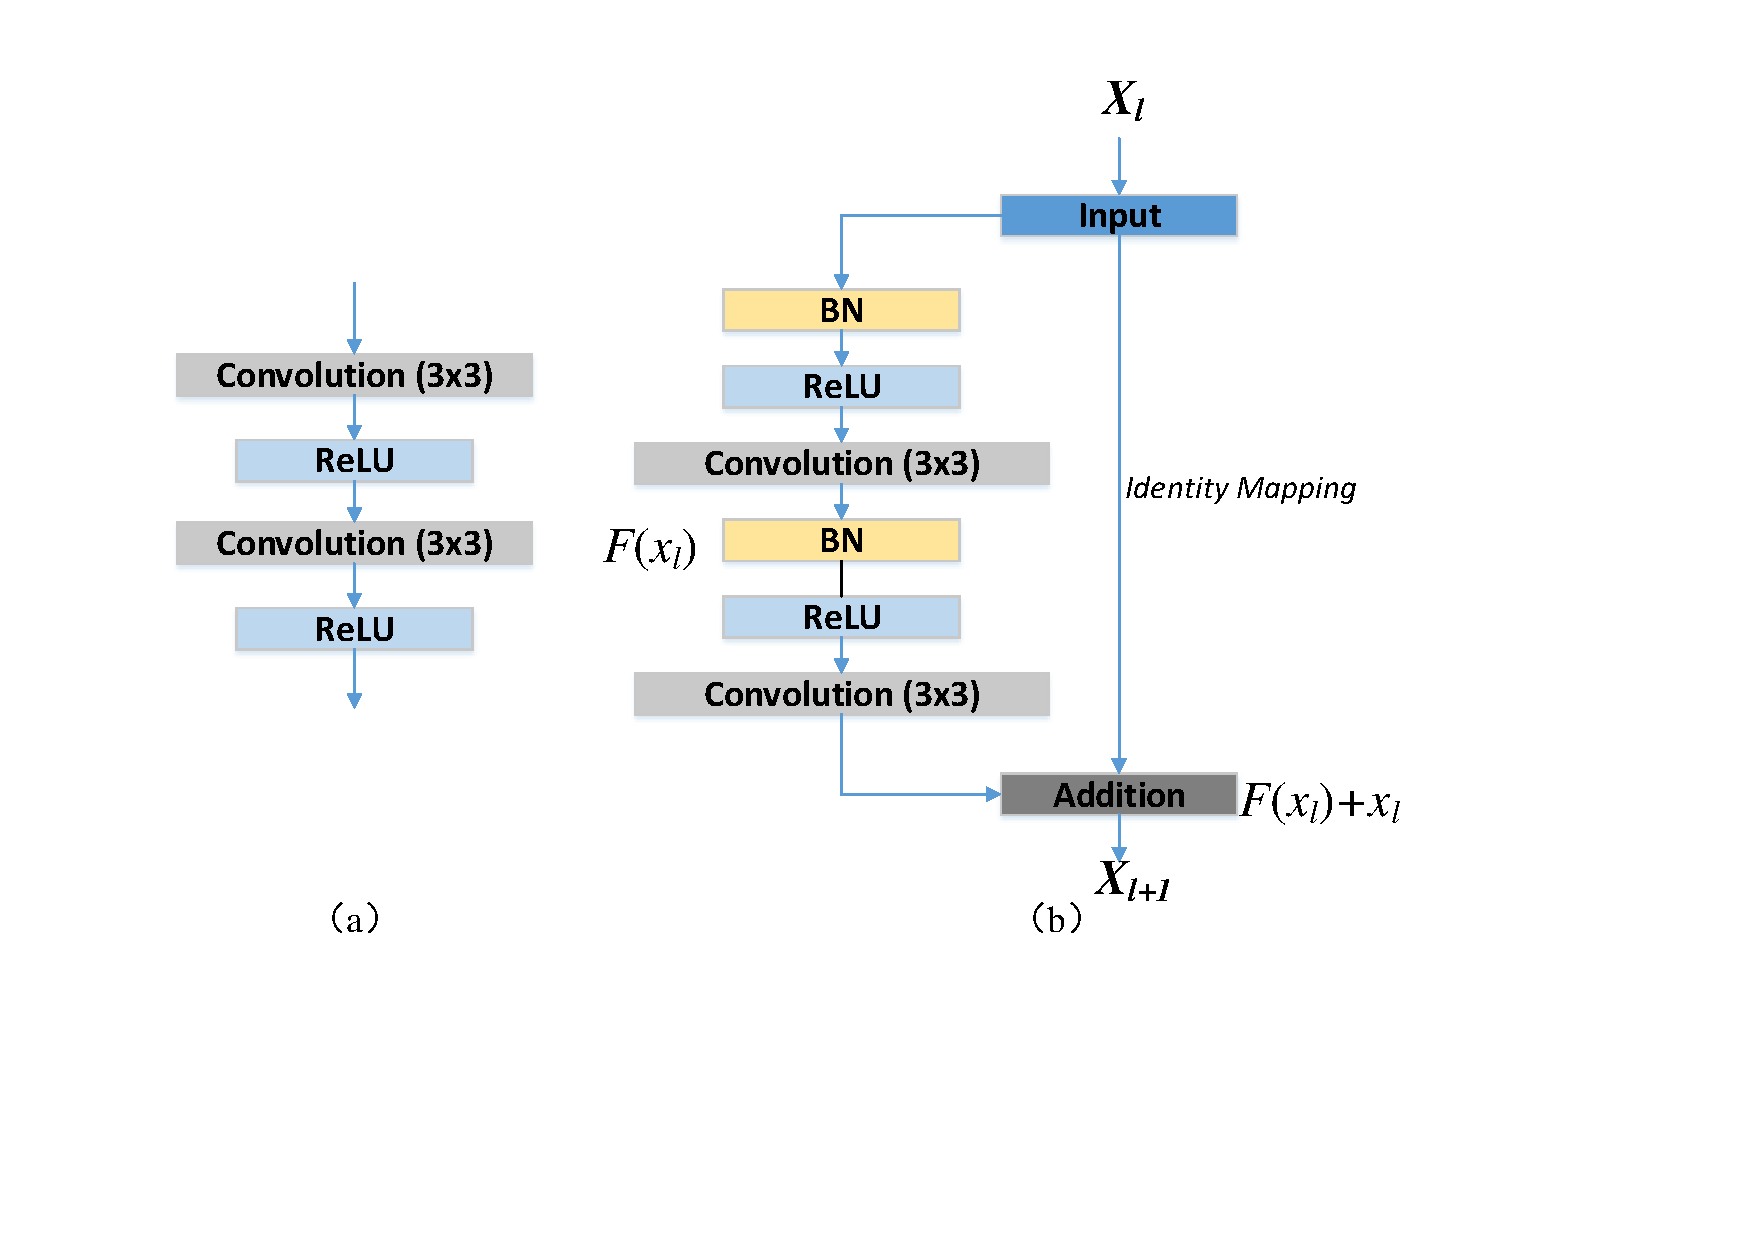
\includegraphics[width=0.6\columnwidth]{res-u-net-blocks.pdf}
		\caption{神经网络的构建模块。(a) U-Net中使用的普通神经单元和(b)本文提出的的ResUnet中使用的具有恒等映射的残差块。}
		\label{Fig:ResNet Block}
	\end{center}
\end{figure}
\subsubsection{残差块}
深入将改善多层神经网络的性能,但可能会妨碍训练,并可能出现退化问题\cite{21}。为了克服这些问题,He等人\cite{21}提出了残差神经网络,以便于训练和解决退化问题。残差神经网络由一系列叠加的残差块组成。每个残差块可表示为一般形式:
\begin{equation}\label{Equ:Residual Uint}
  \begin{split}
  \mathbf{y}_{l}\ \ \ & = h(\mathbf{x}_{l})+\mathcal{F}(\mathbf{x}_{l}, \mathcal{W}_{l}), \\
  \mathbf{x}_{l+1} & = f(\mathbf{y}_{l}),
  \end{split}
\end{equation}
其中$\mathbf{x}_{l}$和$\mathbf{x}_{l+1}$是第$l$个残差块,$\mathcal{F}(\cdot)$是残差函数, $f(\mathbf{y}_l)$是激活函数,$h(\mathbf{x}_{l})$是恒等映射,例如$h(\mathbf{x}_{l}) = \mathbf{x}_{l}$这样的。图~\ref{Fig:ResNet Block}显示了普通单元和残差块之间的差异。在一个残差块中存在批量归一化(BN)、ReLU激活和卷积层的多种组合。He等人\cite{22}详细讨论了不同组合的影响,并提出了完整的预激活设计,如图~\ref{Fig:ResNet Block}(b)所示。在这项工作中,我们还使用全预激活残差块来构建我们的深度残差U-Net网络。
\begin{figure}[tbp!]
	\begin{center}
		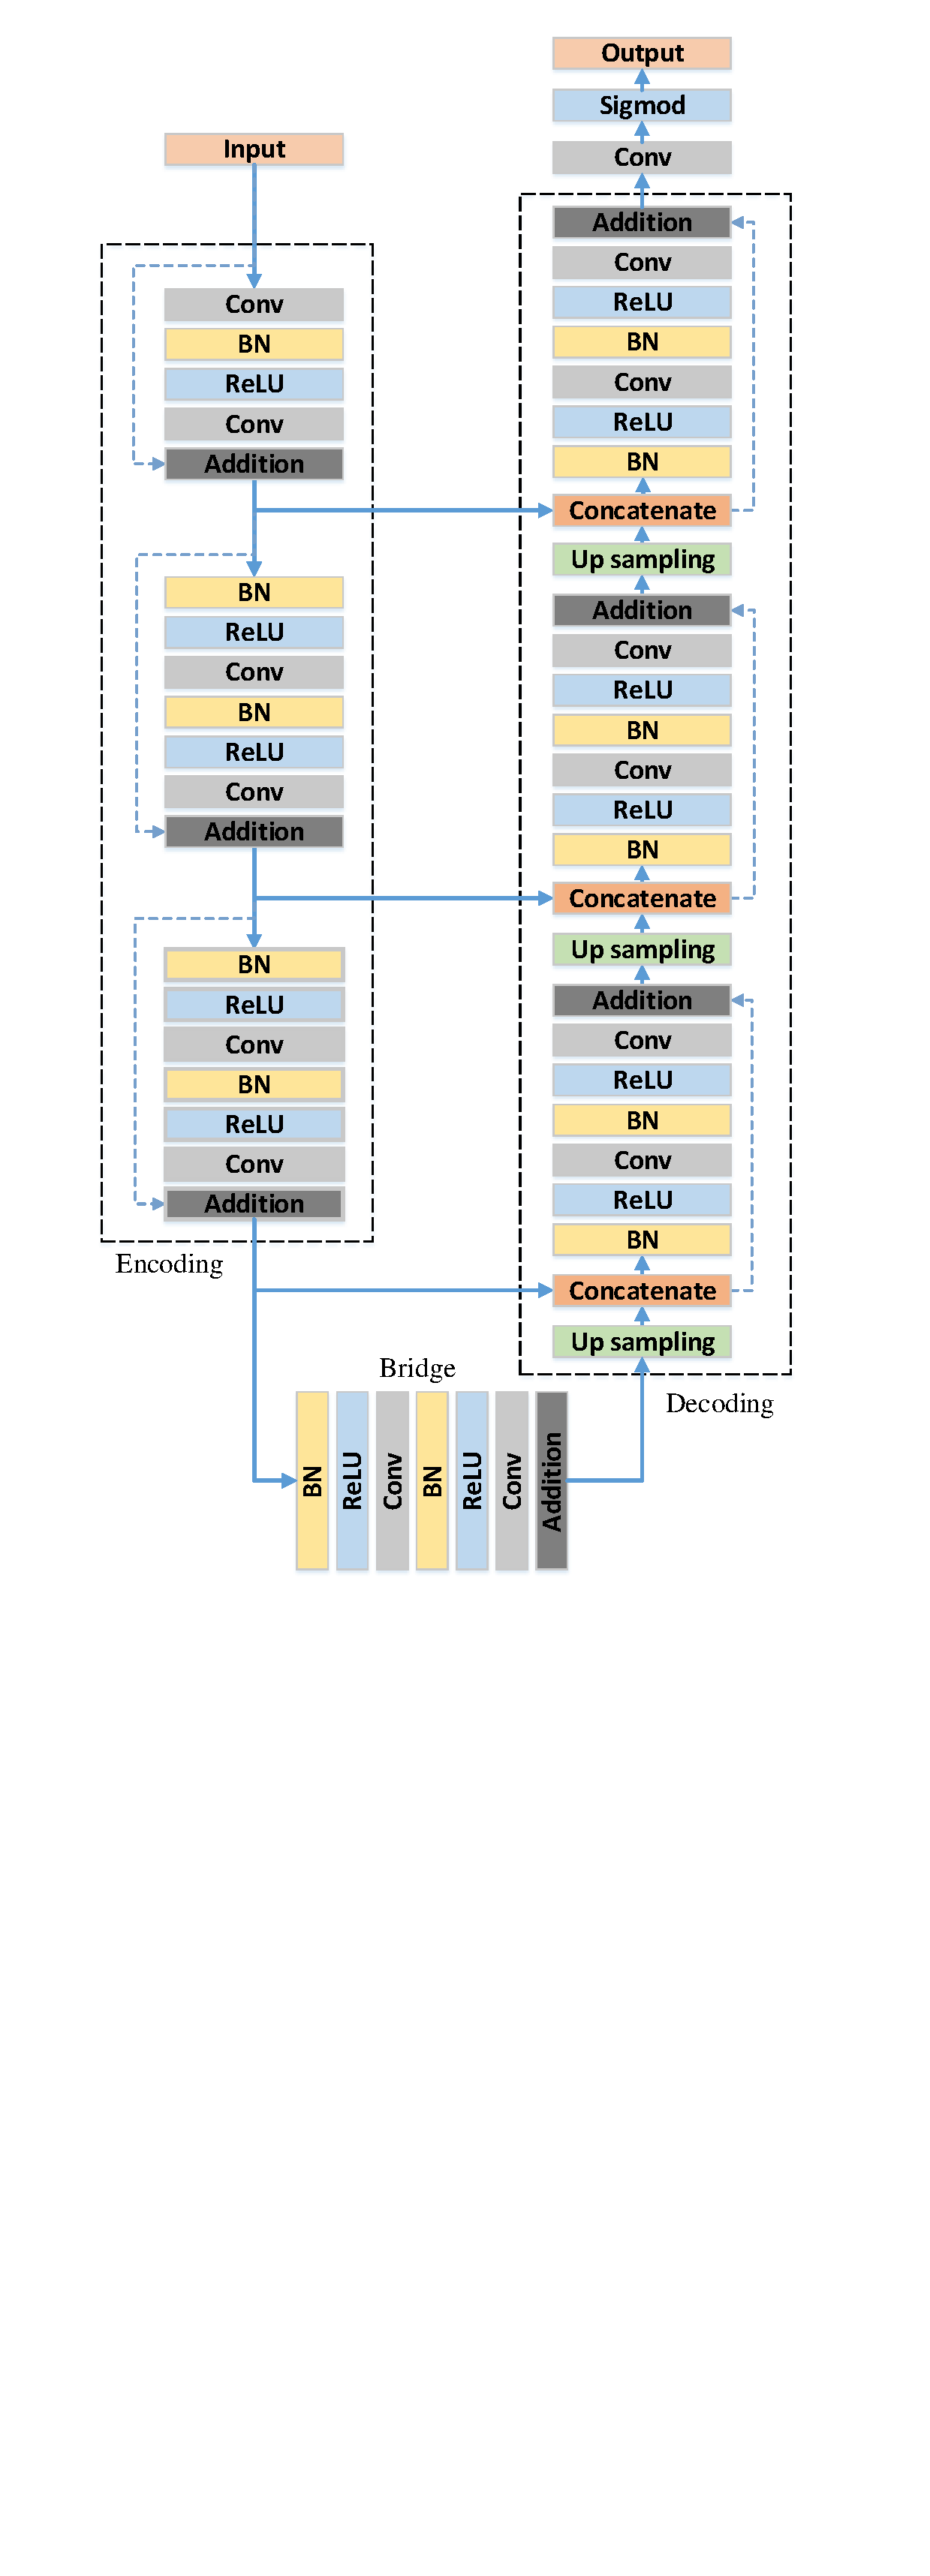
\includegraphics[width=0.6\columnwidth]{ResUNet.pdf}
		\caption{本文提出的ResUnet网络结构}
		\label{Fig:Deep Res-U-Net}
	\end{center}
\end{figure}

\subsubsection{Deep ResUnet}
在这里,我们提出了deep ResUnet,这是一种结合了U-Net和残差神经网络优点的语义分割神经网络。这种组合给我们带来了两个好处:1)残差块将简化网络训练;2)残差块内以及网络低层和高层之间的跳跃连接将促进信息传播而不会退化,从而可以设计参数更少的神经网络,但可以在语义分割方面取得更好的性能。

在这项工作中,我们使用deep ResUnet的7级体系结构进行道路区域提取,如图~\ref{Fig:Deep Res-U-Net}所示。该网络由编码、桥接和反编码三部分组成。\footnote{U-Net使用“收缩”和“扩展”路径来表示网络的特征提取和上卷积阶段。在本文中,我们更喜欢术语编码和解码,因为我们认为它更有意义,更容易理解}第一部分将输入图像编码为紧凑的表示形式。最后一部分将表示恢复为像素级分类,即语义分割。中间部分就像连接编码和解码路径的桥梁。这三个部分都是用残差块构建的,残差块由两个$3\times 3$卷积块和一个单位映射组成。每个卷积块包括BN层、ReLU激活层和卷积层。标识映射连接单元的输入和输出。

编码路径有三个残差块。在每个单元中,不是使用池操作来减小特征映射大小的采样,而是对第一个卷积块执行步长为2的卷积操作,以将特征映射减少一半。相应地,解码路径也由三个残差块组成。在每个单元之前,从较低级别对特征映射进行上采样,并与相应编码路径中的特征映射进行串联。在最后一级解码路径之后,使用$1\times1$卷积和sigmod激活层将多通道特征映射投影到所需的分割中。我们总共有15个卷积层,而U-Net有23个卷积层。值得注意的是,U-Net中不可或缺的裁剪在我们的网络中是不必要的。每个步骤的参数和输出大小如表~\ref{Table:Feature Size}所示。
\begin{table}[!htb]
	\tiny
	\centering
	\caption{ResUnet的网络结构}	
	\label{Table:Feature Size}	
	\begin{tabular}{ccllcl}
		\hline
		\hline
		& Unit level  & Conv layer & Filter  & Stride &  Output size\\
		\hline
		Input                      &        &     &   &    &  $224\times 224 \times 3$ \\
		\hline	
		\multirow{6}{*}{Encoding}
		& \multirow{2}{*}{Level 1}& Conv 1  & $3\times 3/64$ & 1 &  $224\times 224 \times 64$ \\
		&        & Conv 2  &  $3\times 3/64$ & 1 &  $224\times 224 \times 64$ \\
		\cline{2-6}			
		& \multirow{2}{*}{Level 2}& Conv 3  &  $3\times 3/128$ & 2 &  $112\times 112 \times 128$ \\
		&        & Conv 4  &  $3\times 3/128$ & 1 &  $112\times 112 \times 128$ \\
		\cline{2-6}
		& \multirow{2}{*}{Level 3}& Conv 5  &  $3\times 3/256$ & 2 &  $56\times 56 \times 256$ \\
		&        & Conv 6  &  $3\times 3/256$ & 1 &  $56\times 56 \times 256$ \\
		\cline{2-6}						
		\hline
		\multirow{2}{*}{Bridge}
		&\multirow{2}{*}{Level 4}         &Conv 7  &  $3\times 3/512$ & 2 &  $28\times 28 \times 512$ \\
		&	      &Conv 8 &  $3\times 3/512$ & 1 &  $28\times 28 \times 512$\\
		\hline
		\multirow{6}{*}{Decoding}	
		& \multirow{2}{*}{Level 5} &Conv 9 &  $3\times 3/256$ & 1 &  $56\times 56 \times 256$ \\
		&        &Conv 10 &  $3\times 3/256$ & 1 & $56\times 56 \times 256$ \\
		\cline{2-6}
		& \multirow{2}{*}{Level 6} &Conv 11 &  $3\times 3/128$ & 1 &  $112\times 112 \times 128$ \\
		&        &Conv 12 &  $3\times 3/128$ & 1 &  $112\times 112 \times 128$ \\
		\cline{2-6}			
		& \multirow{2}{*}{Level 7} &Conv 13 &  $3\times 3/64$ & 1 &   $224\times 224 \times 64$ \\
		&        &Conv 14 &  $3\times 3/64$ & 1 &  $224\times 224 \times 64$ \\
		\hline
		Output                      &        &Conv 15 &  $1\times 1$ & 1 &  $224\times 224 \times 1$ \\		
		\hline
		\hline
	\end{tabular}
\end{table}

\subsection{损失函数}

给定一组训练图像和相应的地面真值分割$\{I_i,s_i\}$,我们的目标是估计网络的参数$W$,以便生成准确而稳健的道路区域。这是通过最大限度地减少由$Net(I_i;W)$和地面真相$s_i$生成的分段之间的损失来实现的。在本文中,我们使用均方误差(MSE)作为损失函数:
\begin{equation}\label{Equ:mse}
  \mathcal{L}(W) = \frac{1}{N}\sum\limits^{N}_{i=1}||Net(I_i;W) - s_i||^2,
\end{equation}
其中$N$是训练样本数。我们使用随机梯度下降(SGD)来训练我们的网络。众所周知,其他可推导的损耗函数也可用于训练网络。例如,U-Net采用像素交叉熵作为损失函数来优化模型。

\subsection{结果优化}

我们的语义切分网络的输入和输出在宽度和高度上都是相同的,即$224\times224$。由于卷积层中的零填充,输出边界附近的像素精确率会低于中心像素。为了得到更好的分割结果,我们使用了重叠策略来生成大图像的分割结果。输入子图像是从原始图像中裁剪出来的,重叠度为$o$(在我们的实验中$o=14$)。最后的结果是通过将所有子分割拼接在一起得到的。重叠区域中的值会取平均值。

\section{实验}

为了证明所提出的deep ResUnet的准确性和效率,我们在马萨诸塞州道路数据集\footnote{https://www.cs.toronto.edu/\~{}vmnih/data/}上对其进行了测试,并将其与Mnih的~\cite{2}方法、Saito~\cite{5}的方法和U-Net~\cite{24}这三种最新方法作了比较。

\subsection{数据集}

马萨诸塞州道路数据集由Mihn等人建立~\cite{2}。该数据集共包含1171幅图像,其中1108幅用于训练,14幅用于验证,49幅用于测试。此数据集中所有图像的大小为$1500\times1500$像素,分辨率为1.2米/像素。该数据集大致涵盖了从城市、次城市到农村地区的500 km$^2$的空间交叉以及广泛的地物,包括道路、河流、海洋、各种建筑物、植被、学校、桥梁、港口、车辆等。在本文中,我们在该数据集的训练集上训练我们的网络,并在其测试集上报告结果。

\subsection{实现细节}

该模型采用Keras\cite{25}框架实现,并通过SGD算法最小化损失函数.~\ref{Equ:mse}进行优化。有1108张大小为$1500\times1500$的训练图像可用于训练。理论上,我们的网络可以将任意大小的图像作为输入,但是需要大量的GPU内存来存储特征地图。在本文中,我们使用固定大小的训练图像($224\times224$,如表~\ref{Table:Feature Size})来训练模型。这些训练图像是从原始图像中随机抽取的。最后,生成30000个样本并反馈到网络中学习参数。应注意的是,训练期间未使用数据扩充。我们开始在NVIDIA Titan 1080 GPU上以8个小批量训练模型。最初,学习率设置为0.001,每20个周期(epoch)衰减为0.1倍。网络将在50个周期(epoch)内收敛。

\subsection{评价指标}

评估二进制分类方法最常用的指标是精确率和召回率。在遥感中,这些指标也称为正确度和完整度。精确率是预测为道路像素的比率,召回率是正确预测为道路像素的比率。

由于很难正确标记所有道路像素,Mnih等人\cite{2}在道路提取中引入了宽松的精确率和召回率\cite{26}。松弛精确率定义为$\rho$像素范围内预测为道路的像素数与标记为道路的像素数的比率。松弛召回率是标记为道路的像素数与预测为道路的像素数之间$\rho$像素范围内的比率。在本实验中,松弛参数$\rho$设置为3,这与之前的研究\cite{2,5}一致。我们还报告了不同方法的盈亏平衡点。盈亏平衡点定义为松弛精度召回曲线上的点,其精确率值等于召回率。换句话说,盈亏平衡点是松弛精度召回曲线和线y=x的交点。

\subsection{对比研究}

在马萨诸塞州道路数据集的测试集上,我们比较了三种基于深度学习的道路提取方法。表~\ref{Table:Value at Breakeven Point}展示了本文方法和所对比方法的盈亏平衡点。图~\ref{Fig:PR}显示了U-Net和我们的网络的松弛精确率召回曲线及其盈亏平衡点,以及所比较方法的盈亏平衡点。可以看出,我们的方法在松弛精确率和召回率方面优于所有其他三种方法。虽然我们的网络参数仅为U-Net的$1/4$(7.8M vs 30.6M),但在道路提取任务上取得了有希望的改进。

\begin{table}[!hbp]
  \begin{center}
  \caption{在马萨诸塞州道路数据集上,就盈亏平衡点对提出的和其他三种基于深度学习的道路提取方法进行了比较。盈亏平衡点越高,表示在精确率和召回率方面的性能越好。}
  \label{Table:Value at Breakeven Point}
  \begin{tabular}{l|c}
  \hline
  Model & Breakeven point\\
  \hline
  Mnih-CNN\cite{2} & 0.8873  \\
  \hline
  Mnih-CNN+CRF\cite{2} & 0.8904  \\
  \hline
  Mnih-CNN+Post-Processing\cite{2} & 0.9006  \\
  \hline
  Saito-CNN\cite{5} & 0.9047 \\
  \hline
  U-Net\cite{24} & 0.9053 \\
  \hline
  ResUnet & \textbf{0.9187} \\
  \hline
  \end{tabular}
  \end{center}
\end{table}

\begin{figure}[!t]
  \begin{center}
      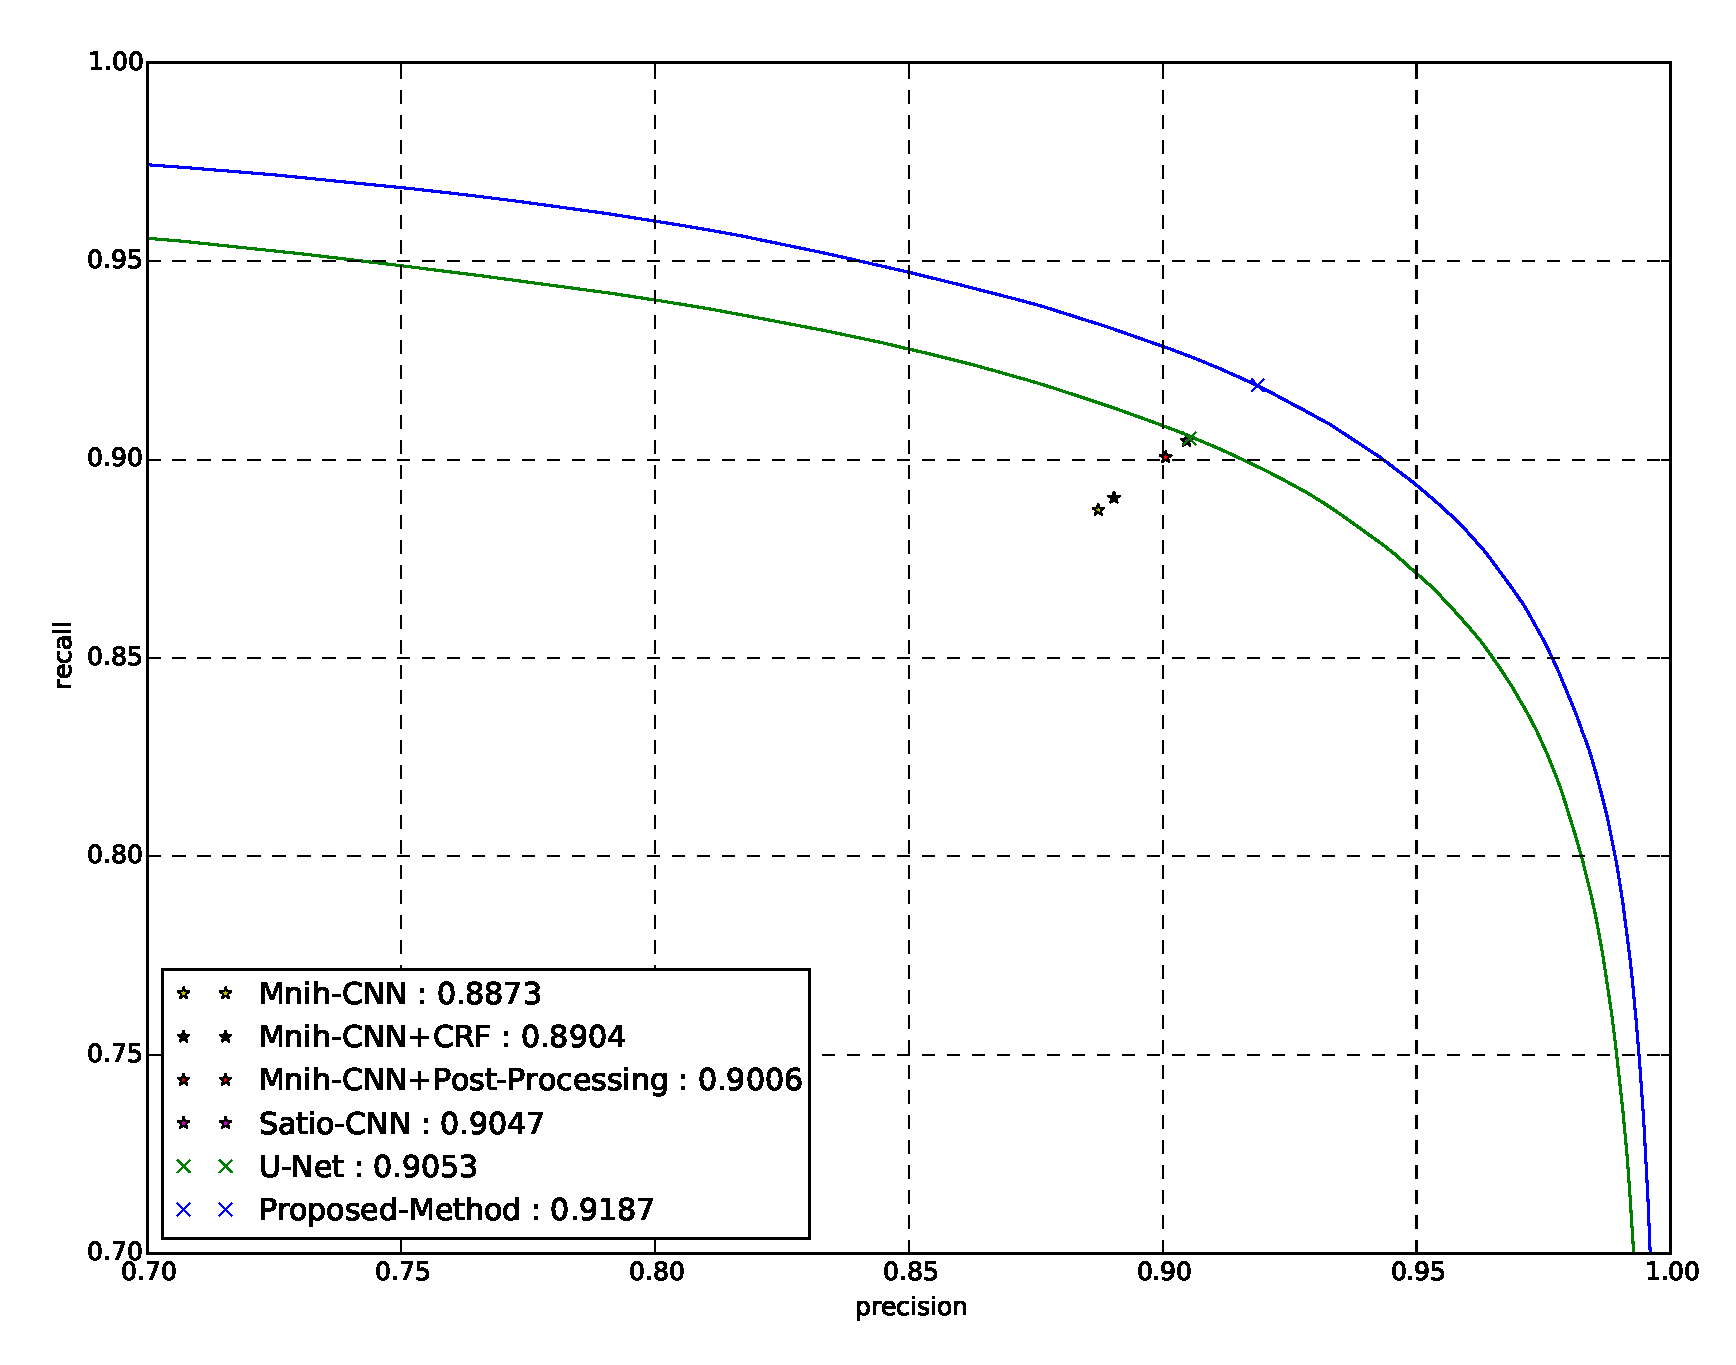
\includegraphics[width=1\columnwidth]{pr1.pdf}
        \caption{U-Net和本文提出的方法的松弛精度召回曲线在马萨诸塞州道路数据集上的对比。标记“$\star$”和“$\times$”的是不同方法的盈亏平衡点。}
        \label{Fig:PR}
  \end{center}
  \end{figure}
  
  \begin{figure*}[ht]
  \begin{center}
      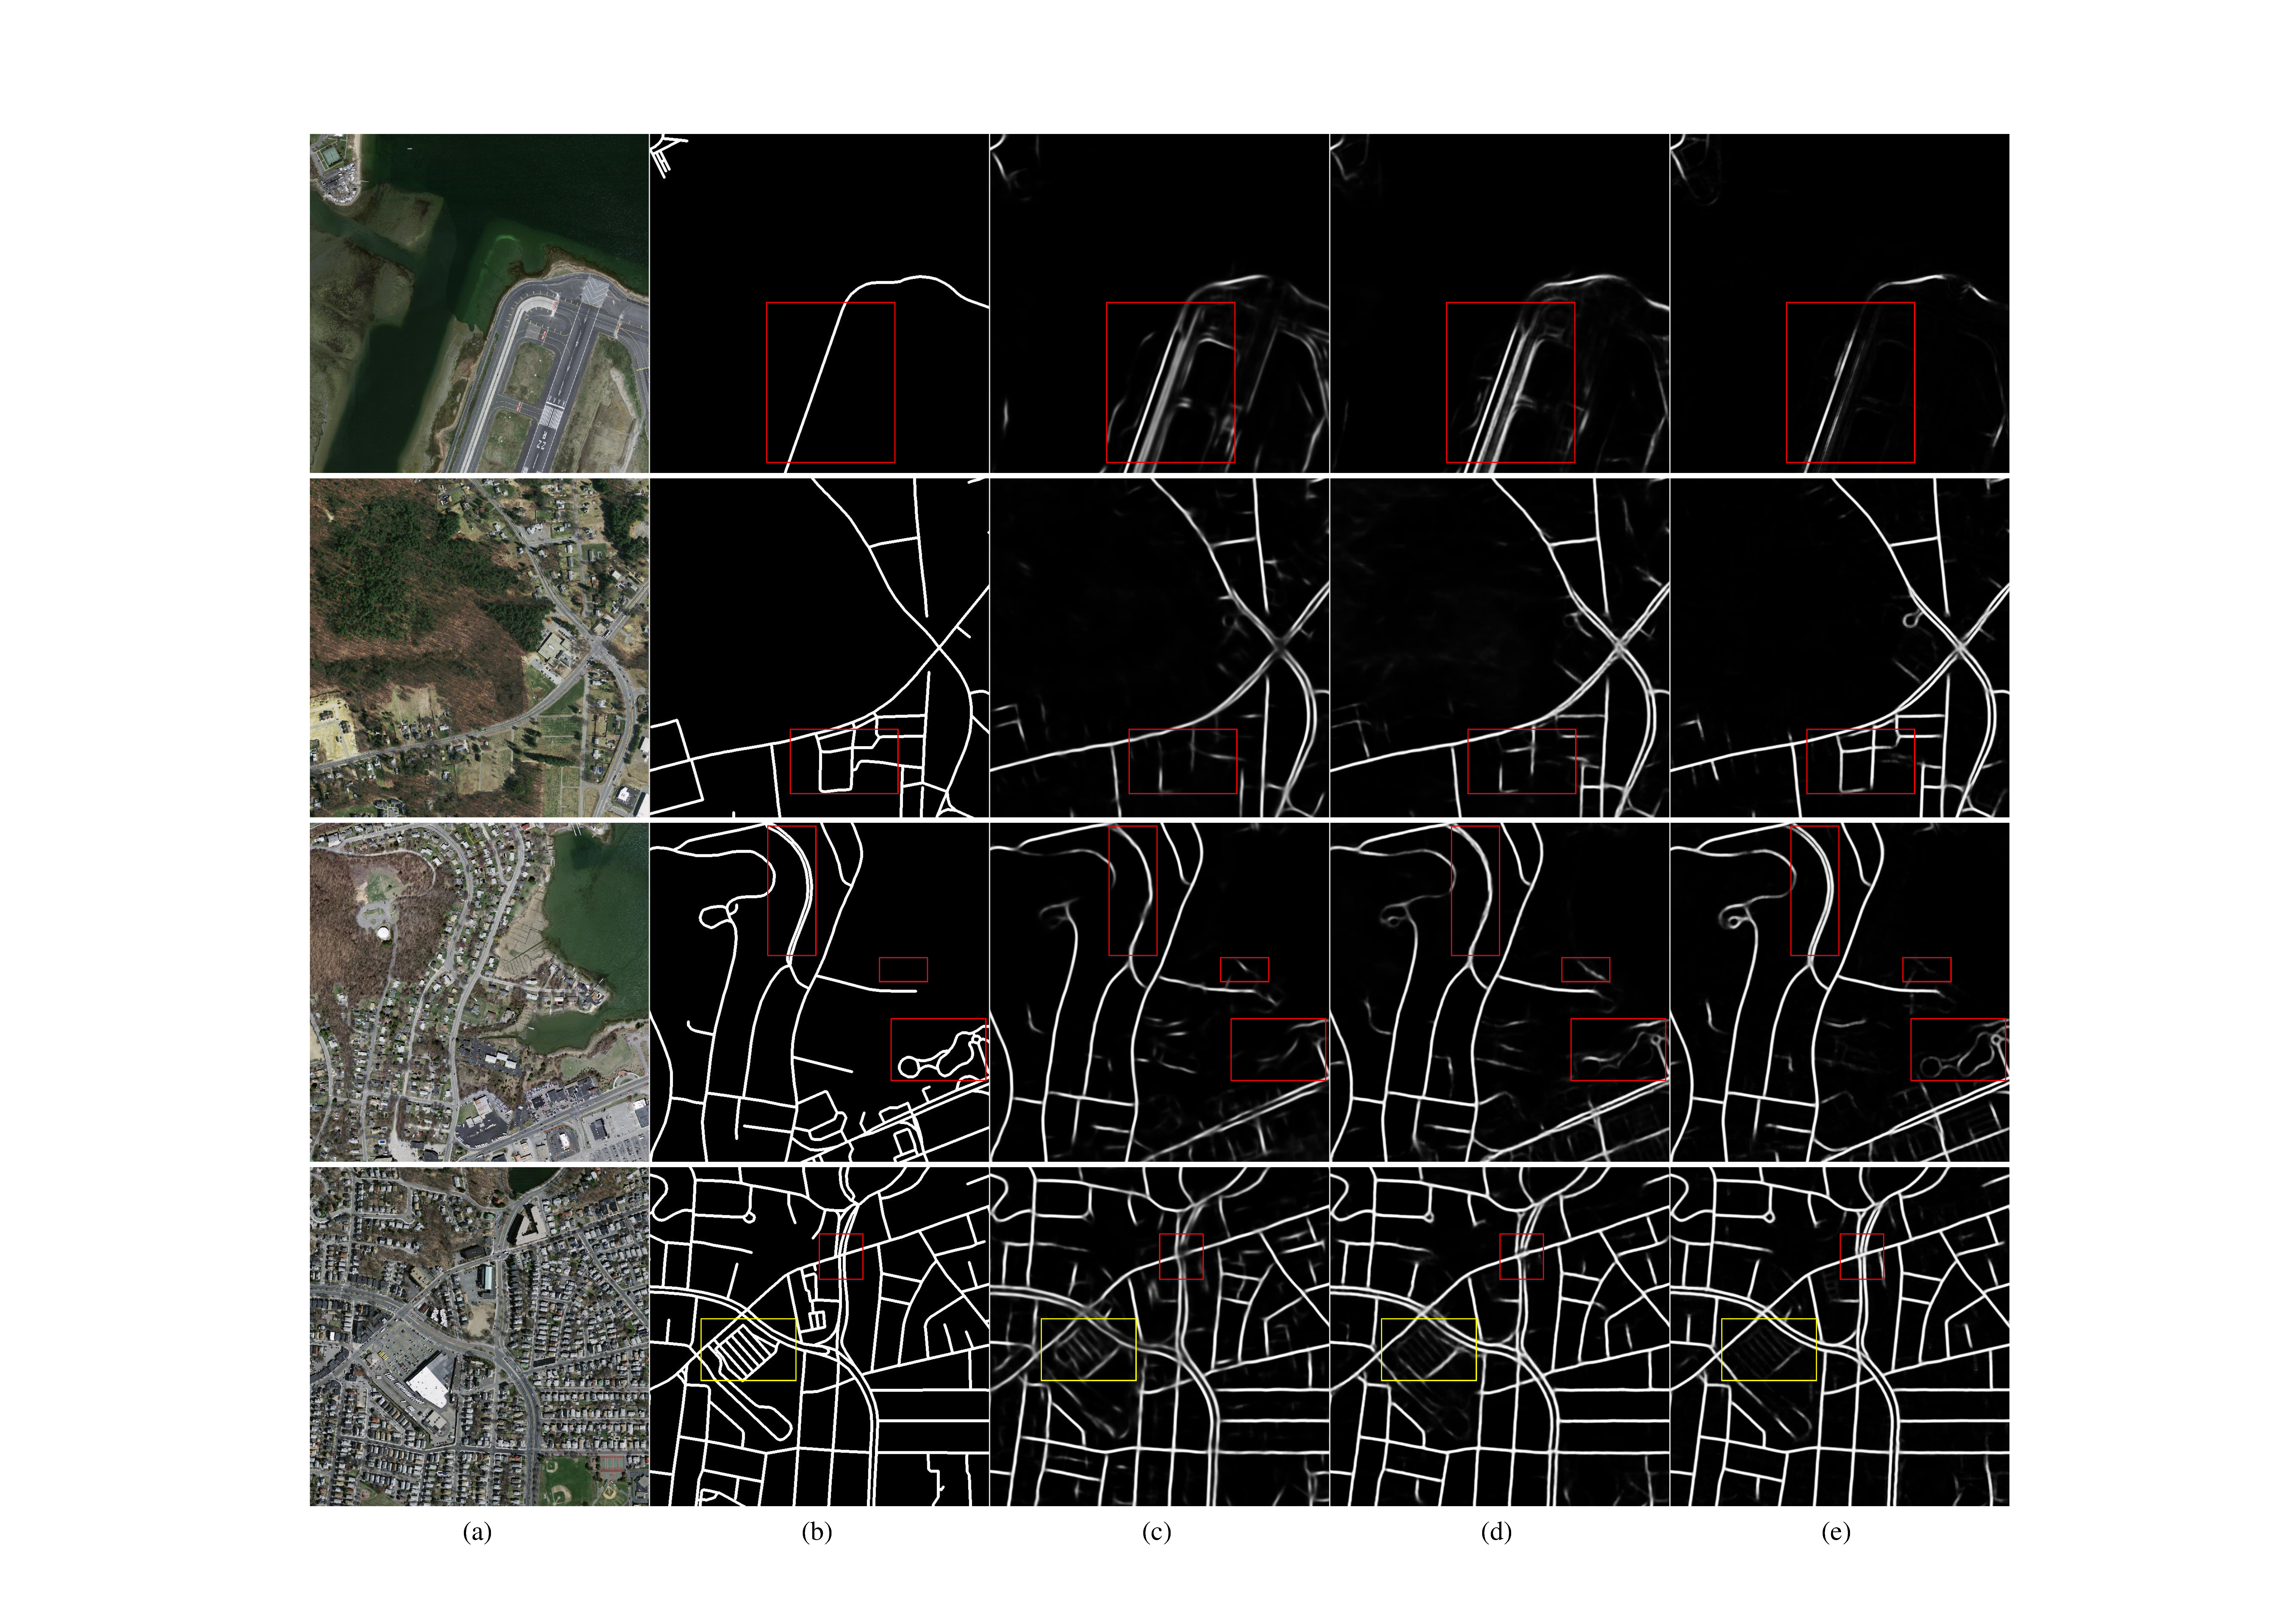
\includegraphics[width=1\textwidth]{imag_compare_2.pdf}
        \caption{马萨诸塞州道路数据集测试集的结果示例。(a) 输入图像;(b) 地面真相;(c) Saito等人~\cite{5};(d) U-Net ~\cite{24};(e) 本文方法结果。放大以查看更多详细信息。}
        \label{Fig:Result Comparison_0}
  \end{center}
\end{figure*}

图~\ref{Fig:Result Comparison_0}展示了Saito等人~\cite{5}的四个示例结果、U-Net~\cite{24}和我们所提出方法的结果。可以看出,与其他两种方法相比,我们的方法显示出更清晰的结果,并且噪声更小。特别是当有两条车道的道路时,我们的方法可以高置信度地分割每条车道,生成干净、清晰的两条车道道路,而其他方法可能会混淆车道,如图~\ref{Fig:Result Comparison_0}的第三行所示。同样,在相交区域,我们的方法也能产生更好的结果。

在分析具有复杂结构的对象时,上下文信息非常重要。我们的网络考虑了道路的上下文信息,因此可以将道路与类似对象(如建筑屋顶、机场跑道)区分开来。从图\ref{Fig:Result Comparison_0}的第一行可以看出,即使跑道具有与公路非常相似的特征,我们的方法也可以成功地从跑道分割出边路。除此之外,上下文信息还使其对遮挡具有鲁棒性。例如,第二行矩形上的部分道路被树木覆盖。Saito的方法和U-Net无法检测树下的道路,但我们的方法成功地标记了它们。故障案例显示在最后一行的黄色矩形中。我们的方法错过了停车场的道路。这主要是因为停车场的大多数道路都没有贴标签。因此,尽管这些道路与普通道路具有相同的特征,但考虑到上下文信息,我们的网络将其视为背景。

\section{结论}

在本文中,我们提出了从高分辨率遥感图像中提取道路的结果。该网络结合了残差学习和U-Net的优点。残差块内以及网络编码和解码路径之间的skip连接将促进了前向和后向计算中的信息传播。这种特性不仅便于训练,而且允许我们设计简单高效的神经网络。该网络的性能优于U-Net,仅需1/4的参数,以及其他两种基于深度学习的道路提取方法。

\appendix

% 书面翻译的参考文献
\bibliographystyle{unsrtnat}
\bibliography{ref/appendix}

% 书面翻译对应的原文索引
\begin{translation-index}
  \nocite{2017Road}
  \bibliographystyle{unsrtnat}
  \bibliography{ref/appendix}
\end{translation-index}

\end{translation}
  % 本科生:外文资料的书面翻译 ++
% % !TeX root = ../thuthesis-example.tex

\chapter{补充内容}

附录是与论文内容密切相关、但编入正文又影响整篇论文编排的条理和逻辑性的资料,例如某些重要的数据表格、计算程序、统计表等,是论文主体的补充内容,可根据需要设置。


\section{图表示例}

\subsection{图}

图~\ref{ResUNet}为所实现的ResUNet网络结构。
\begin{figure}
  \centering
  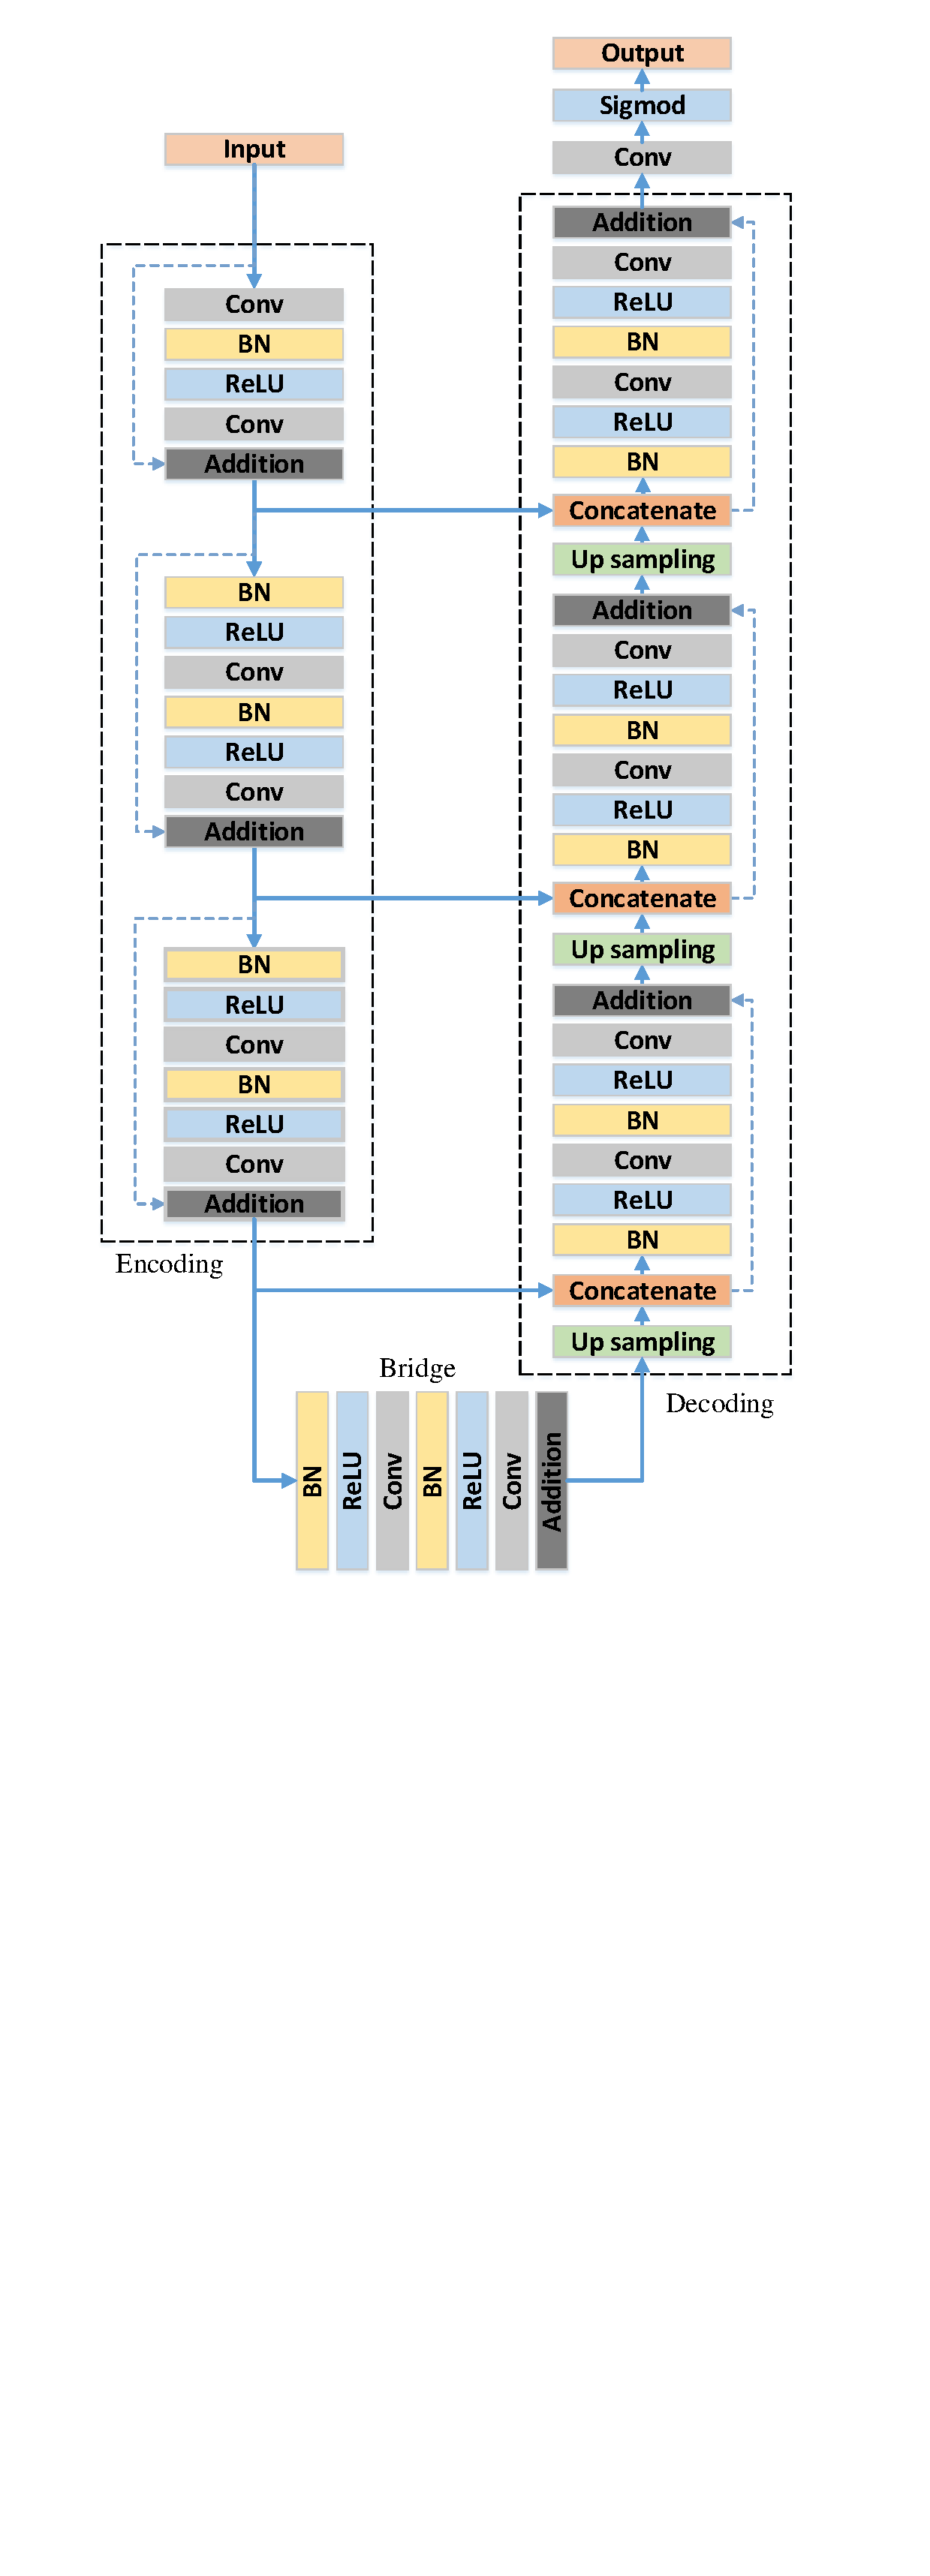
\includegraphics[width=0.5\linewidth]{ResUNet.pdf}
  \caption{ResUNet网络结构}
  \label{ResUNet}
\end{figure}


\subsection{表格}

附录中的表格示例(表~\ref{tab:appendix-table})。

\begin{table}
  \centering
  \caption{附录中的表格示例}
  \begin{tabular}{ll}
    \toprule
    文件名          & 描述                         \\
    \midrule
    thuthesis.dtx   & 模板的源文件,包括文档和注释 \\
    thuthesis.cls   & 模板文件                     \\
    thuthesis-*.bst & BibTeX 参考文献表样式文件    \\
    thuthesis-*.bbx & BibLaTeX 参考文献表样式文件  \\
    thuthesis-*.cbx & BibLaTeX 引用样式文件        \\
    \bottomrule
  \end{tabular}
  \label{tab:appendix-table}
\end{table}


\section{数学公式}

附录中的数学公式示例(公式\eqref{eq:appendix-equation})。
\begin{equation}
  \frac{1}{2 \uppi \symup{i}} \int_\gamma f = \sum_{k=1}^m n(\gamma; a_k) \mathscr{R}(f; a_k)
  \label{eq:appendix-equation}
\end{equation}
 ++


% 个人简历、在学期间完成的相关学术成果
% 本科生可以附个人简历,也可以不附个人简历
% % !TeX root = ../thuthesis-example.tex

\begin{resume}

  \section*{个人简历}

  197× 年 ×× 月 ×× 日出生于四川××县。

  1992 年 9 月考入××大学化学系××化学专业,1996 年 7 月本科毕业并获得理学学士学位。

  1996 年 9 月免试进入清华大学化学系攻读××化学博士至今。


  \section*{在学期间完成的相关学术成果}

  \subsection*{学术论文}

  \begin{achievements}
    \item Yang Y, Ren T L, Zhang L T, et al. Miniature microphone with silicon-based ferroelectric thin films[J]. Integrated Ferroelectrics, 2003, 52:229-235.
    \item 杨轶, 张宁欣, 任天令, 等. 硅基铁电微声学器件中薄膜残余应力的研究[J]. 中国机械工程, 2005, 16(14):1289-1291.
    \item 杨轶, 张宁欣, 任天令, 等. 集成铁电器件中的关键工艺研究[J]. 仪器仪表学报, 2003, 24(S4):192-193.
    \item Yang Y, Ren T L, Zhu Y P, et al. PMUTs for handwriting recognition. In press[J]. (已被Integrated Ferroelectrics录用)
  \end{achievements}


  \subsection*{专利}

  \begin{achievements}
    \item 任天令, 杨轶, 朱一平, 等. 硅基铁电微声学传感器畴极化区域控制和电极连接的方法: 中国, CN1602118A[P]. 2005-03-30.
    \item Ren T L, Yang Y, Zhu Y P, et al. Piezoelectric micro acoustic sensor based on ferroelectric materials: USA, No.11/215, 102[P]. (美国发明专利申请号.)
  \end{achievements}

\end{resume}
 ++

% 指导教师/指导小组学术评语
% 本科生不需要
% % !TeX root = ../thuthesis-example.tex

\begin{comments}
% \begin{comments}[name = {指导小组学术评语}]
% \begin{comments}[name = {Comments from Thesis Supervisor}]
% \begin{comments}[name = {Comments from Thesis Supervision Committee}]

  论文提出了……

\end{comments}


% 答辩委员会决议书
% 本科生不需要
% % !TeX root = ../thuthesis-example.tex

\begin{resolution}

  论文提出了……

  论文取得的主要创新性成果包括:

  1. ……

  2. ……

  3. ……

  论文工作表明作者在×××××具有×××××知识,具有××××能力,论文××××,答辩××××。

  答辩委员会表决,(×票/一致)同意通过论文答辩,并建议授予×××(姓名)×××(门类)学博士/硕士学位。

\end{resolution}


% 本科生的综合论文训练记录表(扫描版)
% \record{file=scan-record.pdf}

\end{document}
